% Options for packages loaded elsewhere
\PassOptionsToPackage{unicode}{hyperref}
\PassOptionsToPackage{hyphens}{url}
\PassOptionsToPackage{dvipsnames,svgnames,x11names}{xcolor}
%
\documentclass[
  letterpaper,
  DIV=11,
  numbers=noendperiod]{scrreprt}

\usepackage{amsmath,amssymb}
\usepackage{iftex}
\ifPDFTeX
  \usepackage[T1]{fontenc}
  \usepackage[utf8]{inputenc}
  \usepackage{textcomp} % provide euro and other symbols
\else % if luatex or xetex
  \usepackage{unicode-math}
  \defaultfontfeatures{Scale=MatchLowercase}
  \defaultfontfeatures[\rmfamily]{Ligatures=TeX,Scale=1}
\fi
\usepackage{lmodern}
\ifPDFTeX\else  
    % xetex/luatex font selection
\fi
% Use upquote if available, for straight quotes in verbatim environments
\IfFileExists{upquote.sty}{\usepackage{upquote}}{}
\IfFileExists{microtype.sty}{% use microtype if available
  \usepackage[]{microtype}
  \UseMicrotypeSet[protrusion]{basicmath} % disable protrusion for tt fonts
}{}
\makeatletter
\@ifundefined{KOMAClassName}{% if non-KOMA class
  \IfFileExists{parskip.sty}{%
    \usepackage{parskip}
  }{% else
    \setlength{\parindent}{0pt}
    \setlength{\parskip}{6pt plus 2pt minus 1pt}}
}{% if KOMA class
  \KOMAoptions{parskip=half}}
\makeatother
\usepackage{xcolor}
\setlength{\emergencystretch}{3em} % prevent overfull lines
\setcounter{secnumdepth}{5}
% Make \paragraph and \subparagraph free-standing
\ifx\paragraph\undefined\else
  \let\oldparagraph\paragraph
  \renewcommand{\paragraph}[1]{\oldparagraph{#1}\mbox{}}
\fi
\ifx\subparagraph\undefined\else
  \let\oldsubparagraph\subparagraph
  \renewcommand{\subparagraph}[1]{\oldsubparagraph{#1}\mbox{}}
\fi

\usepackage{color}
\usepackage{fancyvrb}
\newcommand{\VerbBar}{|}
\newcommand{\VERB}{\Verb[commandchars=\\\{\}]}
\DefineVerbatimEnvironment{Highlighting}{Verbatim}{commandchars=\\\{\}}
% Add ',fontsize=\small' for more characters per line
\usepackage{framed}
\definecolor{shadecolor}{RGB}{241,243,245}
\newenvironment{Shaded}{\begin{snugshade}}{\end{snugshade}}
\newcommand{\AlertTok}[1]{\textcolor[rgb]{0.68,0.00,0.00}{#1}}
\newcommand{\AnnotationTok}[1]{\textcolor[rgb]{0.37,0.37,0.37}{#1}}
\newcommand{\AttributeTok}[1]{\textcolor[rgb]{0.40,0.45,0.13}{#1}}
\newcommand{\BaseNTok}[1]{\textcolor[rgb]{0.68,0.00,0.00}{#1}}
\newcommand{\BuiltInTok}[1]{\textcolor[rgb]{0.00,0.23,0.31}{#1}}
\newcommand{\CharTok}[1]{\textcolor[rgb]{0.13,0.47,0.30}{#1}}
\newcommand{\CommentTok}[1]{\textcolor[rgb]{0.37,0.37,0.37}{#1}}
\newcommand{\CommentVarTok}[1]{\textcolor[rgb]{0.37,0.37,0.37}{\textit{#1}}}
\newcommand{\ConstantTok}[1]{\textcolor[rgb]{0.56,0.35,0.01}{#1}}
\newcommand{\ControlFlowTok}[1]{\textcolor[rgb]{0.00,0.23,0.31}{#1}}
\newcommand{\DataTypeTok}[1]{\textcolor[rgb]{0.68,0.00,0.00}{#1}}
\newcommand{\DecValTok}[1]{\textcolor[rgb]{0.68,0.00,0.00}{#1}}
\newcommand{\DocumentationTok}[1]{\textcolor[rgb]{0.37,0.37,0.37}{\textit{#1}}}
\newcommand{\ErrorTok}[1]{\textcolor[rgb]{0.68,0.00,0.00}{#1}}
\newcommand{\ExtensionTok}[1]{\textcolor[rgb]{0.00,0.23,0.31}{#1}}
\newcommand{\FloatTok}[1]{\textcolor[rgb]{0.68,0.00,0.00}{#1}}
\newcommand{\FunctionTok}[1]{\textcolor[rgb]{0.28,0.35,0.67}{#1}}
\newcommand{\ImportTok}[1]{\textcolor[rgb]{0.00,0.46,0.62}{#1}}
\newcommand{\InformationTok}[1]{\textcolor[rgb]{0.37,0.37,0.37}{#1}}
\newcommand{\KeywordTok}[1]{\textcolor[rgb]{0.00,0.23,0.31}{#1}}
\newcommand{\NormalTok}[1]{\textcolor[rgb]{0.00,0.23,0.31}{#1}}
\newcommand{\OperatorTok}[1]{\textcolor[rgb]{0.37,0.37,0.37}{#1}}
\newcommand{\OtherTok}[1]{\textcolor[rgb]{0.00,0.23,0.31}{#1}}
\newcommand{\PreprocessorTok}[1]{\textcolor[rgb]{0.68,0.00,0.00}{#1}}
\newcommand{\RegionMarkerTok}[1]{\textcolor[rgb]{0.00,0.23,0.31}{#1}}
\newcommand{\SpecialCharTok}[1]{\textcolor[rgb]{0.37,0.37,0.37}{#1}}
\newcommand{\SpecialStringTok}[1]{\textcolor[rgb]{0.13,0.47,0.30}{#1}}
\newcommand{\StringTok}[1]{\textcolor[rgb]{0.13,0.47,0.30}{#1}}
\newcommand{\VariableTok}[1]{\textcolor[rgb]{0.07,0.07,0.07}{#1}}
\newcommand{\VerbatimStringTok}[1]{\textcolor[rgb]{0.13,0.47,0.30}{#1}}
\newcommand{\WarningTok}[1]{\textcolor[rgb]{0.37,0.37,0.37}{\textit{#1}}}

\providecommand{\tightlist}{%
  \setlength{\itemsep}{0pt}\setlength{\parskip}{0pt}}\usepackage{longtable,booktabs,array}
\usepackage{calc} % for calculating minipage widths
% Correct order of tables after \paragraph or \subparagraph
\usepackage{etoolbox}
\makeatletter
\patchcmd\longtable{\par}{\if@noskipsec\mbox{}\fi\par}{}{}
\makeatother
% Allow footnotes in longtable head/foot
\IfFileExists{footnotehyper.sty}{\usepackage{footnotehyper}}{\usepackage{footnote}}
\makesavenoteenv{longtable}
\usepackage{graphicx}
\makeatletter
\def\maxwidth{\ifdim\Gin@nat@width>\linewidth\linewidth\else\Gin@nat@width\fi}
\def\maxheight{\ifdim\Gin@nat@height>\textheight\textheight\else\Gin@nat@height\fi}
\makeatother
% Scale images if necessary, so that they will not overflow the page
% margins by default, and it is still possible to overwrite the defaults
% using explicit options in \includegraphics[width, height, ...]{}
\setkeys{Gin}{width=\maxwidth,height=\maxheight,keepaspectratio}
% Set default figure placement to htbp
\makeatletter
\def\fps@figure{htbp}
\makeatother

\KOMAoption{captions}{tableheading}
\makeatletter
\@ifpackageloaded{bookmark}{}{\usepackage{bookmark}}
\makeatother
\makeatletter
\@ifpackageloaded{caption}{}{\usepackage{caption}}
\AtBeginDocument{%
\ifdefined\contentsname
  \renewcommand*\contentsname{Table of contents}
\else
  \newcommand\contentsname{Table of contents}
\fi
\ifdefined\listfigurename
  \renewcommand*\listfigurename{List of Figures}
\else
  \newcommand\listfigurename{List of Figures}
\fi
\ifdefined\listtablename
  \renewcommand*\listtablename{List of Tables}
\else
  \newcommand\listtablename{List of Tables}
\fi
\ifdefined\figurename
  \renewcommand*\figurename{Figure}
\else
  \newcommand\figurename{Figure}
\fi
\ifdefined\tablename
  \renewcommand*\tablename{Table}
\else
  \newcommand\tablename{Table}
\fi
}
\@ifpackageloaded{float}{}{\usepackage{float}}
\floatstyle{ruled}
\@ifundefined{c@chapter}{\newfloat{codelisting}{h}{lop}}{\newfloat{codelisting}{h}{lop}[chapter]}
\floatname{codelisting}{Listing}
\newcommand*\listoflistings{\listof{codelisting}{List of Listings}}
\makeatother
\makeatletter
\makeatother
\makeatletter
\@ifpackageloaded{caption}{}{\usepackage{caption}}
\@ifpackageloaded{subcaption}{}{\usepackage{subcaption}}
\makeatother
\ifLuaTeX
  \usepackage{selnolig}  % disable illegal ligatures
\fi
\usepackage{bookmark}

\IfFileExists{xurl.sty}{\usepackage{xurl}}{} % add URL line breaks if available
\urlstyle{same} % disable monospaced font for URLs
\hypersetup{
  pdftitle={Programación Avanzada},
  pdfauthor={Luis Miguel de la Cruz Salas},
  colorlinks=true,
  linkcolor={blue},
  filecolor={Maroon},
  citecolor={Blue},
  urlcolor={Blue},
  pdfcreator={LaTeX via pandoc}}

\title{Programación Avanzada}
\author{Luis Miguel de la Cruz Salas}
\date{2023-01-12}

\begin{document}
\maketitle

\renewcommand*\contentsname{Table of contents}
{
\hypersetup{linkcolor=}
\setcounter{tocdepth}{2}
\tableofcontents
}
\bookmarksetup{startatroot}

\chapter*{Introducción}\label{introducciuxf3n}
\addcontentsline{toc}{chapter}{Introducción}

\markboth{Introducción}{Introducción}

Cuadernos interactivos para la asignatura de Programación Avanzada.

Los Jupyter Notebooks de este curso se pueden obtener en
\url{https://github.com/repomacti/macti/notebooks/}.

\bookmarksetup{startatroot}

\chapter{\texorpdfstring{Espacio vectorial
\(\mathbb{R}^2\).}{Espacio vectorial \textbackslash mathbb\{R\}\^{}2.}}\label{espacio-vectorial-mathbbr2.}

\textbf{Objetivo.} Revisar e ilustrar las propiedades del espacio
vectorial \(\mathbb{R}^2\) usando la biblioteca \texttt{numpy}.

MACTI-Algebra\_Lineal\_01 by Luis M. de la Cruz is licensed under
Attribution-ShareAlike 4.0 International

Trabajo realizado con el apoyo del Programa UNAM-DGAPA-PAPIME PE101922

\section{\texorpdfstring{Vectores en
\(\mathbb{R}^2\).}{Vectores en \textbackslash mathbb\{R\}\^{}2.}}\label{vectores-en-mathbbr2.}

Usando la biblioteca \texttt{numpy} podemos definir vectores en varias
dimensiones. Para ejemplificar definiremos vectores en \(\mathbb{R}^2\)
y haremos algunas operaciones en este espacio vectorial.

\begin{Shaded}
\begin{Highlighting}[]
\CommentTok{\# Importamos las bibliotecas requeridas}
\ImportTok{import}\NormalTok{ numpy }\ImportTok{as}\NormalTok{ np}
\ImportTok{import}\NormalTok{ macti.visual }\ImportTok{as}\NormalTok{ mvis}
\end{Highlighting}
\end{Shaded}

\begin{Shaded}
\begin{Highlighting}[]
\CommentTok{\# Definimos dos vectores en R\^{}2 (arreglos 1D de numpy de longitud 2).}
\NormalTok{x }\OperatorTok{=}\NormalTok{ np.array([}\FloatTok{0.5}\NormalTok{, }\FloatTok{1.0}\NormalTok{])}
\NormalTok{y }\OperatorTok{=}\NormalTok{ np.array([}\FloatTok{1.5}\NormalTok{, }\FloatTok{0.5}\NormalTok{])}

\BuiltInTok{print}\NormalTok{(}\StringTok{\textquotesingle{}x = }\SpecialCharTok{\{\}}\StringTok{\textquotesingle{}}\NormalTok{.}\BuiltInTok{format}\NormalTok{(x))}
\BuiltInTok{print}\NormalTok{(}\StringTok{\textquotesingle{}y = }\SpecialCharTok{\{\}}\StringTok{\textquotesingle{}}\NormalTok{.}\BuiltInTok{format}\NormalTok{(y))}
\end{Highlighting}
\end{Shaded}

\begin{verbatim}
x = [0.5 1. ]
y = [1.5 0.5]
\end{verbatim}

La biblioteca \texttt{macti.visual} permite graficar los vectores en
\(\mathbb{R}^2\) como sigue:

\begin{Shaded}
\begin{Highlighting}[]
\NormalTok{v }\OperatorTok{=}\NormalTok{ mvis.Plotter()  }\CommentTok{\# Definición de un objeto para crear figuras.}
\NormalTok{v.set\_coordsys(}\DecValTok{1}\NormalTok{)   }\CommentTok{\# Definición del sistema de coordenadas.}
\NormalTok{v.plot\_vectors(}\DecValTok{1}\NormalTok{, [x, y], [}\StringTok{\textquotesingle{}x\textquotesingle{}}\NormalTok{, }\StringTok{\textquotesingle{}y\textquotesingle{}}\NormalTok{]) }\CommentTok{\# Graficación de los vectores \textquotesingle{}x\textquotesingle{} y \textquotesingle{}y\textquotesingle{}.}
\NormalTok{v.grid()  }\CommentTok{\# Muestra la rejilla del sistema de coordenadas.}
\end{Highlighting}
\end{Shaded}

\includegraphics{01_Espacios_Vectoriales_files/figure-pdf/cell-4-output-1.png}

\section{Propiedades de un espacio
vectorial.}\label{propiedades-de-un-espacio-vectorial.}

\begin{enumerate}
\def\labelenumi{\arabic{enumi}.}
\tightlist
\item
  \(\vec{x} + \vec{y} \in \mathbb{R}^n\).
\item
  \(\vec{x} + \vec{y} = \vec{y} + \vec{x}\).
\item
  \(\vec{x} + (\vec{y} + \vec{z})= (\vec{x} + \vec{y}) + \vec{z}\).
\item
  Existe el vector neutro \(\vec{0} \in \mathbb{R}^n\) tal que
  \(\vec{x} + \vec{0} = \vec{x}\).
\item
  Para cada \(\vec{x}\in \mathbb{R}^n\) existe el opuesto \(-\vec{x}\)
  tal que \(\vec{x} + (-\vec{x}) = \vec{0}\).
\item
  \(\alpha \vec{x} \in \mathbb{R}^n\).
\item
  \(\alpha (\vec{x} + \vec{y}) = \alpha \vec{x} + \alpha \vec{y}\).
\item
  \((\alpha + \beta) \vec{x} = \alpha \vec{x} + \beta \vec{x}\).
\item
  \(\alpha (\beta \vec{x}) = (\alpha \beta) \vec{x}\).
\item
  Existe el elemento neutro \(\mathbf{1} \in \mathbb{R}\) tal que
  \(\mathbf{1} \vec{x} = \vec{x}\).
\end{enumerate}

\subsection{Propiedad 1: la suma es una operación
interna.}\label{propiedad-1-la-suma-es-una-operaciuxf3n-interna.}

\(\vec{x} + \vec{y} \in \mathbb{R}^n\).

\begin{Shaded}
\begin{Highlighting}[]
\CommentTok{\# Suma de dos vectores}
\NormalTok{z }\OperatorTok{=}\NormalTok{ x }\OperatorTok{+}\NormalTok{ y}

\BuiltInTok{print}\NormalTok{(}\StringTok{\textquotesingle{}x = }\SpecialCharTok{\{\}}\StringTok{\textquotesingle{}}\NormalTok{.}\BuiltInTok{format}\NormalTok{(x))}
\BuiltInTok{print}\NormalTok{(}\StringTok{\textquotesingle{}y = }\SpecialCharTok{\{\}}\StringTok{\textquotesingle{}}\NormalTok{.}\BuiltInTok{format}\NormalTok{(y))}
\BuiltInTok{print}\NormalTok{(}\StringTok{\textquotesingle{}z = x + y = }\SpecialCharTok{\{\}}\StringTok{\textquotesingle{}}\NormalTok{.}\BuiltInTok{format}\NormalTok{(z))}

\CommentTok{\# Graficamos los vectores y su suma}
\NormalTok{v }\OperatorTok{=}\NormalTok{ mvis.Plotter()}
\NormalTok{v.set\_coordsys()}
\NormalTok{v.plot\_vectors\_sum(}\DecValTok{1}\NormalTok{, [x, y], [}\StringTok{\textquotesingle{}x\textquotesingle{}}\NormalTok{, }\StringTok{\textquotesingle{}y\textquotesingle{}}\NormalTok{], ofx}\OperatorTok{={-}}\FloatTok{0.3}\NormalTok{) }\CommentTok{\# Grafica los vectores y el resultado de la suma.}
\NormalTok{v.grid()}
\end{Highlighting}
\end{Shaded}

\begin{verbatim}
x = [0.5 1. ]
y = [1.5 0.5]
z = x + y = [2.  1.5]
\end{verbatim}

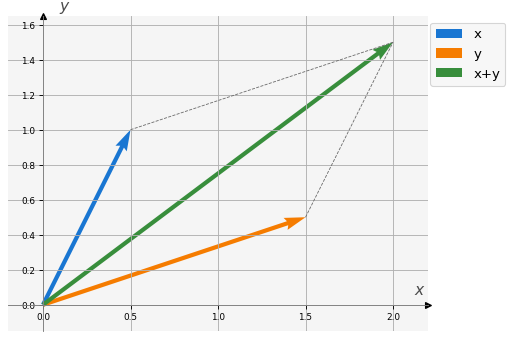
\includegraphics{01_Espacios_Vectoriales_files/figure-pdf/cell-5-output-2.png}

Observa que la función \texttt{plot\_vectors\_sum()} muestra los
vectores originales y la suma de ellos. El nuevo vector \(\vec{z}\) está
en \(\mathbb{R}^2\).

\subsection{Propiedad 2: la suma es
conmutativa.}\label{propiedad-2-la-suma-es-conmutativa.}

\(\vec{x} + \vec{y} = \vec{y} + \vec{x}\).

\begin{Shaded}
\begin{Highlighting}[]
\NormalTok{xpy }\OperatorTok{=}\NormalTok{ x }\OperatorTok{+}\NormalTok{ y}
\NormalTok{ypx }\OperatorTok{=}\NormalTok{ y }\OperatorTok{+}\NormalTok{ x}
\BuiltInTok{print}\NormalTok{(}\StringTok{\textquotesingle{} x + y = }\SpecialCharTok{\{\}}\StringTok{ }\CharTok{\textbackslash{}t}\StringTok{ y + x = }\SpecialCharTok{\{\}}\StringTok{\textquotesingle{}}\NormalTok{.}\BuiltInTok{format}\NormalTok{(xpy, ypx))}
\BuiltInTok{print}\NormalTok{(}\StringTok{\textquotesingle{}}\CharTok{\textbackslash{}n}\StringTok{ ¿ x + y == y + x ? : }\SpecialCharTok{\{\}}\StringTok{\textquotesingle{}}\NormalTok{.}\BuiltInTok{format}\NormalTok{(np.isclose(xpy, ypx)))}
\end{Highlighting}
\end{Shaded}

\begin{verbatim}
 x + y = [2.  1.5]   y + x = [2.  1.5]

 ¿ x + y == y + x ? : [ True  True]
\end{verbatim}

Observa que la operación suma \texttt{+} se realiza componente a
componente.

La función \texttt{np.isclose()} compara cada componente de los arreglos
y determina que tan ``parecidas'' son hasta una tolerancia absoluta de
\(10^{-8}\). Esta forma de comparación es la más conveniente cuando se
comparan números reales (punto flotante, floating point).

\subsection{Propiedad 3: la suma es
asociativa.}\label{propiedad-3-la-suma-es-asociativa.}

\(\vec{x} + (\vec{y} + \vec{z})= (\vec{x} + \vec{y}) + \vec{z}\).

\begin{Shaded}
\begin{Highlighting}[]
\BuiltInTok{print}\NormalTok{(}\StringTok{\textquotesingle{} x = }\SpecialCharTok{\{\}}\StringTok{ }\CharTok{\textbackslash{}t}\StringTok{ y = }\SpecialCharTok{\{\}}\StringTok{ }\CharTok{\textbackslash{}t}\StringTok{ z = }\SpecialCharTok{\{\}}\StringTok{\textquotesingle{}}\NormalTok{.}\BuiltInTok{format}\NormalTok{(x, y, z))}
\BuiltInTok{print}\NormalTok{(}\StringTok{\textquotesingle{} x + (y + z)= }\SpecialCharTok{\{\}}\StringTok{ }\CharTok{\textbackslash{}t}\StringTok{ (x + y) + z = }\SpecialCharTok{\{\}}\StringTok{\textquotesingle{}}\NormalTok{.}\BuiltInTok{format}\NormalTok{(x }\OperatorTok{+}\NormalTok{ (y }\OperatorTok{+}\NormalTok{ z), (x }\OperatorTok{+}\NormalTok{ y) }\OperatorTok{+}\NormalTok{ z))}
\BuiltInTok{print}\NormalTok{(}\StringTok{\textquotesingle{}}\CharTok{\textbackslash{}n}\StringTok{ ¿ x + (y + z) == (x + y) + z : }\SpecialCharTok{\{\}}\StringTok{\textquotesingle{}}\NormalTok{.}\BuiltInTok{format}\NormalTok{(np.isclose(x }\OperatorTok{+}\NormalTok{ (y }\OperatorTok{+}\NormalTok{ z), (x }\OperatorTok{+}\NormalTok{ y) }\OperatorTok{+}\NormalTok{ z)))}
\end{Highlighting}
\end{Shaded}

\begin{verbatim}
 x = [0.5 1. ]   y = [1.5 0.5]   z = [2.  1.5]
 x + (y + z)= [4. 3.]    (x + y) + z = [4. 3.]

 ¿ x + (y + z) == (x + y) + z : [ True  True]
\end{verbatim}

\subsection{Propiedad 4: elemento neutro de la
suma.}\label{propiedad-4-elemento-neutro-de-la-suma.}

Existe el vector neutro \(\vec{0} \in \mathbb{R}^n\) tal que
\(\vec{x} + \vec{0} = \vec{x}\).

\begin{Shaded}
\begin{Highlighting}[]
\CommentTok{\# Definimos el vector neutro.}
\NormalTok{cero }\OperatorTok{=}\NormalTok{ np.zeros(}\DecValTok{2}\NormalTok{)}

\BuiltInTok{print}\NormalTok{(}\StringTok{\textquotesingle{} x = }\SpecialCharTok{\{\}}\StringTok{ }\CharTok{\textbackslash{}t}\StringTok{ cero = }\SpecialCharTok{\{\}}\StringTok{\textquotesingle{}}\NormalTok{.}\BuiltInTok{format}\NormalTok{(x, cero))}
\BuiltInTok{print}\NormalTok{(}\StringTok{\textquotesingle{} x + cero = }\SpecialCharTok{\{\}}\StringTok{\textquotesingle{}}\NormalTok{.}\BuiltInTok{format}\NormalTok{(x }\OperatorTok{+}\NormalTok{ cero))}
\end{Highlighting}
\end{Shaded}

\begin{verbatim}
 x = [0.5 1. ]   cero = [0. 0.]
 x + cero = [0.5 1. ]
\end{verbatim}

\subsection{Propiedad 5: elemento inverso en la
suma.}\label{propiedad-5-elemento-inverso-en-la-suma.}

Para cada \(\vec{x}\in \mathbb{R}^n\) existe el inverso \(-\vec{x}\) tal
que \(\vec{x} + (-\vec{x}) = \vec{0}\).

\begin{Shaded}
\begin{Highlighting}[]
\BuiltInTok{print}\NormalTok{(}\StringTok{\textquotesingle{} x = }\SpecialCharTok{\{\}}\StringTok{ }\CharTok{\textbackslash{}t}\StringTok{ {-}x = }\SpecialCharTok{\{\}}\StringTok{\textquotesingle{}}\NormalTok{.}\BuiltInTok{format}\NormalTok{(x, }\OperatorTok{{-}}\NormalTok{x))}
\BuiltInTok{print}\NormalTok{(}\StringTok{\textquotesingle{} x + ({-}x) = }\SpecialCharTok{\{\}}\StringTok{\textquotesingle{}}\NormalTok{.}\BuiltInTok{format}\NormalTok{(x }\OperatorTok{+}\NormalTok{ (}\OperatorTok{{-}}\NormalTok{x)))}
\end{Highlighting}
\end{Shaded}

\begin{verbatim}
 x = [0.5 1. ]   -x = [-0.5 -1. ]
 x + (-x) = [0. 0.]
\end{verbatim}

\subsection{Propiedad 6: la multiplicación de un vector por un escalar
produce un
vector.}\label{propiedad-6-la-multiplicaciuxf3n-de-un-vector-por-un-escalar-produce-un-vector.}

\(\alpha \vec{x} \in \mathbb{R}^n\).

\begin{Shaded}
\begin{Highlighting}[]
\CommentTok{\# Definimos un escalar}
\NormalTok{α }\OperatorTok{=} \FloatTok{1.5}

\CommentTok{\# Realizamos la multiplicación de x por el escalar}
\NormalTok{αx }\OperatorTok{=}\NormalTok{ α }\OperatorTok{*}\NormalTok{ x}

\CommentTok{\# Mostramos el resultado}
\BuiltInTok{print}\NormalTok{(}\StringTok{\textquotesingle{} α = }\SpecialCharTok{\{\}}\StringTok{ }\CharTok{\textbackslash{}t}\StringTok{ x = }\SpecialCharTok{\{\}}\StringTok{ }\CharTok{\textbackslash{}n}\StringTok{ α * x = }\SpecialCharTok{\{\}}\StringTok{  }\CharTok{\textbackslash{}n}\StringTok{ \textquotesingle{}}\NormalTok{.}\BuiltInTok{format}\NormalTok{(α, x, αx))}

\CommentTok{\# Graficamos el vector original y el resultado.}
\NormalTok{v }\OperatorTok{=}\NormalTok{ mvis.Plotter()}
\NormalTok{v.set\_coordsys()}
\NormalTok{v.plot\_vectors(}\DecValTok{1}\NormalTok{, [x, αx], [}\StringTok{\textquotesingle{}x\textquotesingle{}}\NormalTok{, }\StringTok{\textquotesingle{}αx\textquotesingle{}}\NormalTok{], w}\OperatorTok{=}\FloatTok{0.020}\NormalTok{)}
\NormalTok{v.grid()}
\end{Highlighting}
\end{Shaded}

\begin{verbatim}
 α = 1.5     x = [0.5 1. ] 
 α * x = [0.75 1.5 ]  
 
\end{verbatim}

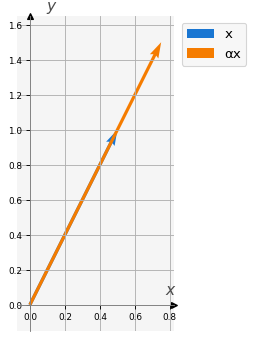
\includegraphics{01_Espacios_Vectoriales_files/figure-pdf/cell-10-output-2.png}

Observa que el vector original \(\vec{x} = (0.5, 1.0)\), representado
por la flecha azul, es más pequeño que el vector resultante
\(\alpha \vec{x} = (0.75, 1.5)\), representado por la flecha naranja.
\(\alpha\) multiplica a cada componente del vector \(\vec{x}\). Cuando
multiplicamos un vector por un escalar, puede ocurrir que su longitud se
agrande, se reduzca y/o que cambie de sentido. Intenta modificar el
valor de \(\alpha\) a \(0.5\) y luego a \(-0.5\), observa que sucede.

\subsection{Propiedad 7: distributividad
I.}\label{propiedad-7-distributividad-i.}

\(\alpha (\vec{x} + \vec{y}) = \alpha \vec{x} + \alpha \vec{y}\)

\begin{Shaded}
\begin{Highlighting}[]
\BuiltInTok{print}\NormalTok{(}\StringTok{\textquotesingle{} α = }\SpecialCharTok{\{\}}\StringTok{\textquotesingle{}}\NormalTok{.}\BuiltInTok{format}\NormalTok{(α))}
\BuiltInTok{print}\NormalTok{(}\StringTok{\textquotesingle{} x = }\SpecialCharTok{\{\}}\StringTok{ }\CharTok{\textbackslash{}t}\StringTok{ y = }\SpecialCharTok{\{\}}\StringTok{\textquotesingle{}}\NormalTok{.}\BuiltInTok{format}\NormalTok{(x, y))}
\BuiltInTok{print}\NormalTok{(}\StringTok{\textquotesingle{} α * (x + y) = }\SpecialCharTok{\{\}}\StringTok{\textquotesingle{}}\NormalTok{.}\BuiltInTok{format}\NormalTok{(α }\OperatorTok{*}\NormalTok{ (x }\OperatorTok{+}\NormalTok{ y)))}
\BuiltInTok{print}\NormalTok{(}\StringTok{\textquotesingle{} α * x + α * y = }\SpecialCharTok{\{\}}\StringTok{\textquotesingle{}}\NormalTok{.}\BuiltInTok{format}\NormalTok{(α }\OperatorTok{*}\NormalTok{ x }\OperatorTok{+}\NormalTok{ α }\OperatorTok{*}\NormalTok{ y))}
\BuiltInTok{print}\NormalTok{(}\StringTok{\textquotesingle{} ¿ α * (x + y) == α * x + α * y ? : }\SpecialCharTok{\{\}}\StringTok{\textquotesingle{}}\NormalTok{.}\BuiltInTok{format}\NormalTok{(np.isclose(α }\OperatorTok{*}\NormalTok{ (x }\OperatorTok{+}\NormalTok{ y), α }\OperatorTok{*}\NormalTok{ x }\OperatorTok{+}\NormalTok{ α }\OperatorTok{*}\NormalTok{ y)))}
\end{Highlighting}
\end{Shaded}

\begin{verbatim}
 α = 1.5
 x = [0.5 1. ]   y = [1.5 0.5]
 α * (x + y) = [3.   2.25]
 α * x + α * y = [3.   2.25]
 ¿ α * (x + y) == α * x + α * y ? : [ True  True]
\end{verbatim}

\subsection{Propiedad 8: distributividad
II.}\label{propiedad-8-distributividad-ii.}

\((\alpha + \beta) \vec{x} = \alpha \vec{x} + \beta \vec{x}\)

\begin{Shaded}
\begin{Highlighting}[]
\CommentTok{\# Definimos dos escalares}
\NormalTok{α }\OperatorTok{=} \FloatTok{2.0}
\NormalTok{β }\OperatorTok{=} \FloatTok{1.5}

\BuiltInTok{print}\NormalTok{(}\StringTok{\textquotesingle{} α = }\SpecialCharTok{\{\}}\StringTok{ }\CharTok{\textbackslash{}t}\StringTok{ β = }\SpecialCharTok{\{\}}\StringTok{ }\CharTok{\textbackslash{}t}\StringTok{ α + β = }\SpecialCharTok{\{\}}\StringTok{\textquotesingle{}}\NormalTok{.}\BuiltInTok{format}\NormalTok{(α, β, α }\OperatorTok{+}\NormalTok{ β))}
\BuiltInTok{print}\NormalTok{(}\StringTok{\textquotesingle{} x = }\SpecialCharTok{\{\}}\StringTok{\textquotesingle{}}\NormalTok{.}\BuiltInTok{format}\NormalTok{(x))}
\BuiltInTok{print}\NormalTok{(}\StringTok{\textquotesingle{} (α + β) * x = }\SpecialCharTok{\{\}}\StringTok{\textquotesingle{}}\NormalTok{.}\BuiltInTok{format}\NormalTok{((α }\OperatorTok{+}\NormalTok{ β) }\OperatorTok{*}\NormalTok{ x))}
\BuiltInTok{print}\NormalTok{(}\StringTok{\textquotesingle{} α * x + β * x = }\SpecialCharTok{\{\}}\StringTok{\textquotesingle{}}\NormalTok{.}\BuiltInTok{format}\NormalTok{(α }\OperatorTok{*}\NormalTok{ x }\OperatorTok{+}\NormalTok{ β }\OperatorTok{*}\NormalTok{ x))}
\BuiltInTok{print}\NormalTok{(}\StringTok{\textquotesingle{} ¿ (α + β) * x == α * x + β * x ? : }\SpecialCharTok{\{\}}\StringTok{\textquotesingle{}}\NormalTok{.}\BuiltInTok{format}\NormalTok{(np.isclose((α }\OperatorTok{+}\NormalTok{ β) }\OperatorTok{*}\NormalTok{ x, α }\OperatorTok{*}\NormalTok{ x }\OperatorTok{+}\NormalTok{ β }\OperatorTok{*}\NormalTok{ x)))}
\end{Highlighting}
\end{Shaded}

\begin{verbatim}
 α = 2.0     β = 1.5     α + β = 3.5
 x = [0.5 1. ]
 (α + β) * x = [1.75 3.5 ]
 α * x + β * x = [1.75 3.5 ]
 ¿ (α + β) * x == α * x + β * x ? : [ True  True]
\end{verbatim}

\subsection{Propiedad 9.
asociatividad.}\label{propiedad-9.-asociatividad.}

\(\alpha (\beta \vec{x}) = (\alpha \beta) \vec{x}\).

\begin{Shaded}
\begin{Highlighting}[]
\CommentTok{\# Definimos dos escalares}
\NormalTok{α }\OperatorTok{=} \FloatTok{2.0}
\NormalTok{β }\OperatorTok{=} \FloatTok{1.5}

\BuiltInTok{print}\NormalTok{(}\StringTok{\textquotesingle{} α = }\SpecialCharTok{\{\}}\StringTok{ }\CharTok{\textbackslash{}t}\StringTok{ β = }\SpecialCharTok{\{\}}\StringTok{ }\CharTok{\textbackslash{}t}\StringTok{ x = }\SpecialCharTok{\{\}}\StringTok{\textquotesingle{}}\NormalTok{.}\BuiltInTok{format}\NormalTok{(α, β, x))}
\BuiltInTok{print}\NormalTok{(}\StringTok{\textquotesingle{} α * (β * x) = }\SpecialCharTok{\{\}}\StringTok{\textquotesingle{}}\NormalTok{.}\BuiltInTok{format}\NormalTok{(α }\OperatorTok{*}\NormalTok{ ( β }\OperatorTok{*}\NormalTok{ x)))}
\BuiltInTok{print}\NormalTok{(}\StringTok{\textquotesingle{} (α * β) * x = }\SpecialCharTok{\{\}}\StringTok{\textquotesingle{}}\NormalTok{.}\BuiltInTok{format}\NormalTok{((α }\OperatorTok{*}\NormalTok{ β) }\OperatorTok{*}\NormalTok{ x))}
\BuiltInTok{print}\NormalTok{(}\StringTok{\textquotesingle{} ¿ α * (β * x) == (α * β) * x ? : }\SpecialCharTok{\{\}}\StringTok{\textquotesingle{}}\NormalTok{.}\BuiltInTok{format}\NormalTok{(np.isclose(α }\OperatorTok{*}\NormalTok{ (β }\OperatorTok{*}\NormalTok{ x), (α }\OperatorTok{*}\NormalTok{ β) }\OperatorTok{*}\NormalTok{ x)))}
\end{Highlighting}
\end{Shaded}

\begin{verbatim}
 α = 2.0     β = 1.5     x = [0.5 1. ]
 α * (β * x) = [1.5 3. ]
 (α * β) * x = [1.5 3. ]
 ¿ α * (β * x) == (α * β) * x ? : [ True  True]
\end{verbatim}

\subsection{Propiedad 10.}\label{propiedad-10.}

Existe el elemento neutro \(\mathbf{1} \in \mathbb{R}\) tal que
\(\mathbf{1} \vec{x} = \vec{x}\).

\begin{Shaded}
\begin{Highlighting}[]
\NormalTok{α }\OperatorTok{=} \FloatTok{1.0}

\BuiltInTok{print}\NormalTok{(}\StringTok{\textquotesingle{} α = }\SpecialCharTok{\{\}}\StringTok{ }\CharTok{\textbackslash{}t}\StringTok{ x = }\SpecialCharTok{\{\}}\StringTok{\textquotesingle{}}\NormalTok{.}\BuiltInTok{format}\NormalTok{(α, x))}
\BuiltInTok{print}\NormalTok{(}\StringTok{\textquotesingle{} α * x = }\SpecialCharTok{\{\}}\StringTok{\textquotesingle{}}\NormalTok{.}\BuiltInTok{format}\NormalTok{(α }\OperatorTok{*}\NormalTok{ x))}
\BuiltInTok{print}\NormalTok{(}\StringTok{\textquotesingle{} ¿ α * x == x ? : }\SpecialCharTok{\{\}}\StringTok{\textquotesingle{}}\NormalTok{.}\BuiltInTok{format}\NormalTok{(np.isclose(α }\OperatorTok{*}\NormalTok{ x, x)))}
\end{Highlighting}
\end{Shaded}

\begin{verbatim}
 α = 1.0     x = [0.5 1. ]
 α * x = [0.5 1. ]
 ¿ α * x == x ? : [ True  True]
\end{verbatim}

\section{\texorpdfstring{\textbf{Ejercicio
1.}}{Ejercicio 1.}}\label{ejercicio-1.}

Definimos los siguientes vectores \(\vec{x} = (1.2, 3.4, 5.2, -6.7)\) y
\(\vec{y} = (4.4, -2.3, 5.3, 8.9)\) ambos en \(\mathbb{R}^4\). Usando
\(\alpha = 0.5\) y \(\beta = 3.5\), verifica que se cumplen las
propiedades 1 a 10 para \(\vec{x}\) y \(\vec{y}\). Hint. Define los
vectores \(\vec{x}\) y \(\vec{y}\) usando \texttt{numpy} y
posteriormente copia los códigos utilizados en el ejemplo de
\(\mathbb{R}^2\) para cada propiedad. En algunos casos debes ajustar el
código para este ejercicio. Obervación. En este caso no es posible
realizar gráficas.

\begin{Shaded}
\begin{Highlighting}[]
\CommentTok{\#\#\# Definición de los vectores en R\^{}4 con numpy}
\NormalTok{x }\OperatorTok{=}\NormalTok{ np.array([}\FloatTok{1.2}\NormalTok{, }\FloatTok{3.4}\NormalTok{, }\FloatTok{5.2}\NormalTok{, }\OperatorTok{{-}}\FloatTok{6.7}\NormalTok{])}
\NormalTok{y }\OperatorTok{=}\NormalTok{ np.array([}\FloatTok{4.4}\NormalTok{, }\OperatorTok{{-}}\FloatTok{2.3}\NormalTok{, }\FloatTok{5.3}\NormalTok{, }\FloatTok{8.9}\NormalTok{])}

\BuiltInTok{print}\NormalTok{(}\StringTok{\textquotesingle{}x = }\SpecialCharTok{\{\}}\StringTok{\textquotesingle{}}\NormalTok{.}\BuiltInTok{format}\NormalTok{(x))}
\BuiltInTok{print}\NormalTok{(}\StringTok{\textquotesingle{}y = }\SpecialCharTok{\{\}}\StringTok{\textquotesingle{}}\NormalTok{.}\BuiltInTok{format}\NormalTok{(y))}
\end{Highlighting}
\end{Shaded}

\begin{verbatim}
x = [ 1.2  3.4  5.2 -6.7]
y = [ 4.4 -2.3  5.3  8.9]
\end{verbatim}

\textbf{Propiedad 1.}

El resultado debería ser:

\begin{verbatim}
x = [ 1.2  3.4  5.2 -6.7]
y = [ 4.4 -2.3  5.3  8.9]
z = x + y = [ 5.6  1.1 10.5  2.2]
\end{verbatim}

\begin{Shaded}
\begin{Highlighting}[]
\CommentTok{\#\#\# Propiedad 1.}

\CommentTok{\#\#\# }\RegionMarkerTok{BEGIN}\CommentTok{ SOLUTION}
\NormalTok{z }\OperatorTok{=}\NormalTok{ x }\OperatorTok{+}\NormalTok{ y}

\BuiltInTok{print}\NormalTok{(}\StringTok{\textquotesingle{}x = }\SpecialCharTok{\{\}}\StringTok{\textquotesingle{}}\NormalTok{.}\BuiltInTok{format}\NormalTok{(x))}
\BuiltInTok{print}\NormalTok{(}\StringTok{\textquotesingle{}y = }\SpecialCharTok{\{\}}\StringTok{\textquotesingle{}}\NormalTok{.}\BuiltInTok{format}\NormalTok{(y))}
\BuiltInTok{print}\NormalTok{(}\StringTok{\textquotesingle{}z = x + y = }\SpecialCharTok{\{\}}\StringTok{\textquotesingle{}}\NormalTok{.}\BuiltInTok{format}\NormalTok{(z))}
\CommentTok{\#\#\# }\RegionMarkerTok{END}\CommentTok{ SOLUTION}
\end{Highlighting}
\end{Shaded}

\begin{verbatim}
x = [ 1.2  3.4  5.2 -6.7]
y = [ 4.4 -2.3  5.3  8.9]
z = x + y = [ 5.6  1.1 10.5  2.2]
\end{verbatim}

\textbf{Propiedad 2.}

El resultado debería ser:

\begin{verbatim}
 x + y = [ 5.6  1.1 10.5  2.2]   y + x = [ 5.6  1.1 10.5  2.2]

 ¿ x + y == y + x ? : [ True  True  True  True]
\end{verbatim}

\begin{Shaded}
\begin{Highlighting}[]
\CommentTok{\#\#\# Propiedad 2.}

\CommentTok{\#\#\# }\RegionMarkerTok{BEGIN}\CommentTok{ SOLUTION}
\NormalTok{xpy }\OperatorTok{=}\NormalTok{ x }\OperatorTok{+}\NormalTok{ y}
\NormalTok{ypx }\OperatorTok{=}\NormalTok{ y }\OperatorTok{+}\NormalTok{ x}
\BuiltInTok{print}\NormalTok{(}\StringTok{\textquotesingle{} x + y = }\SpecialCharTok{\{\}}\StringTok{ }\CharTok{\textbackslash{}t}\StringTok{ y + x = }\SpecialCharTok{\{\}}\StringTok{\textquotesingle{}}\NormalTok{.}\BuiltInTok{format}\NormalTok{(xpy, ypx))}
\BuiltInTok{print}\NormalTok{(}\StringTok{\textquotesingle{}}\CharTok{\textbackslash{}n}\StringTok{ ¿ x + y == y + x ? : }\SpecialCharTok{\{\}}\StringTok{\textquotesingle{}}\NormalTok{.}\BuiltInTok{format}\NormalTok{(xpy }\OperatorTok{==}\NormalTok{ ypx))}
\CommentTok{\#\#\# }\RegionMarkerTok{END}\CommentTok{ SOLUTION}
\end{Highlighting}
\end{Shaded}

\begin{verbatim}
 x + y = [ 5.6  1.1 10.5  2.2]   y + x = [ 5.6  1.1 10.5  2.2]

 ¿ x + y == y + x ? : [ True  True  True  True]
\end{verbatim}

\textbf{Propiedad 3.}

El resultado debería ser:

\begin{verbatim}
 x = [ 1.2  3.4  5.2 -6.7]   y = [ 4.4 -2.3  5.3  8.9]   z = [ 5.6  1.1 10.5  2.2]
 x + (y + z)= [11.2  2.2 21.   4.4]      (x + y) + z = [11.2  2.2 21.   4.4]

 ¿ x + (y + z) == (x + y) + z : [ True  True  True  True]
\end{verbatim}

\begin{Shaded}
\begin{Highlighting}[]
\CommentTok{\#\#\# Propiedad 3.}

\CommentTok{\#\#\# }\RegionMarkerTok{BEGIN}\CommentTok{ SOLUTION}
\BuiltInTok{print}\NormalTok{(}\StringTok{\textquotesingle{} x = }\SpecialCharTok{\{\}}\StringTok{ }\CharTok{\textbackslash{}t}\StringTok{ y = }\SpecialCharTok{\{\}}\StringTok{ }\CharTok{\textbackslash{}t}\StringTok{ z = }\SpecialCharTok{\{\}}\StringTok{\textquotesingle{}}\NormalTok{.}\BuiltInTok{format}\NormalTok{(x, y, z))}
\BuiltInTok{print}\NormalTok{(}\StringTok{\textquotesingle{} x + (y + z)= }\SpecialCharTok{\{\}}\StringTok{ }\CharTok{\textbackslash{}t}\StringTok{ (x + y) + z = }\SpecialCharTok{\{\}}\StringTok{\textquotesingle{}}\NormalTok{.}\BuiltInTok{format}\NormalTok{(x }\OperatorTok{+}\NormalTok{ (y }\OperatorTok{+}\NormalTok{ z), (x }\OperatorTok{+}\NormalTok{ y) }\OperatorTok{+}\NormalTok{ z))}
\BuiltInTok{print}\NormalTok{(}\StringTok{\textquotesingle{}}\CharTok{\textbackslash{}n}\StringTok{ ¿ x + (y + z) == (x + y) + z : }\SpecialCharTok{\{\}}\StringTok{\textquotesingle{}}\NormalTok{.}\BuiltInTok{format}\NormalTok{(np.isclose(x }\OperatorTok{+}\NormalTok{ (y }\OperatorTok{+}\NormalTok{ z), (x }\OperatorTok{+}\NormalTok{ y) }\OperatorTok{+}\NormalTok{ z)))}
\CommentTok{\#\#\# }\RegionMarkerTok{END}\CommentTok{ SOLUTION}
\end{Highlighting}
\end{Shaded}

\begin{verbatim}
 x = [ 1.2  3.4  5.2 -6.7]   y = [ 4.4 -2.3  5.3  8.9]   z = [ 5.6  1.1 10.5  2.2]
 x + (y + z)= [11.2  2.2 21.   4.4]      (x + y) + z = [11.2  2.2 21.   4.4]

 ¿ x + (y + z) == (x + y) + z : [ True  True  True  True]
\end{verbatim}

\textbf{Propiedad 4.}

El resultado debería ser:

\begin{verbatim}
 x = [ 1.2  3.4  5.2 -6.7]   cero = [0. 0. 0. 0.]
 x + cero = [ 1.2  3.4  5.2 -6.7]
\end{verbatim}

\begin{Shaded}
\begin{Highlighting}[]
\CommentTok{\#\#\# Propiedad 4.}

\CommentTok{\#\#\# }\RegionMarkerTok{BEGIN}\CommentTok{ SOLUTION}
\NormalTok{cero }\OperatorTok{=}\NormalTok{ np.zeros(}\DecValTok{4}\NormalTok{)}
\BuiltInTok{print}\NormalTok{(}\StringTok{\textquotesingle{} x = }\SpecialCharTok{\{\}}\StringTok{ }\CharTok{\textbackslash{}t}\StringTok{ cero = }\SpecialCharTok{\{\}}\StringTok{\textquotesingle{}}\NormalTok{.}\BuiltInTok{format}\NormalTok{(x, cero))}
\BuiltInTok{print}\NormalTok{(}\StringTok{\textquotesingle{} x + cero = }\SpecialCharTok{\{\}}\StringTok{\textquotesingle{}}\NormalTok{.}\BuiltInTok{format}\NormalTok{(x }\OperatorTok{+}\NormalTok{ cero))}
\CommentTok{\#\#\# }\RegionMarkerTok{END}\CommentTok{ SOLUTION}
\end{Highlighting}
\end{Shaded}

\begin{verbatim}
 x = [ 1.2  3.4  5.2 -6.7]   cero = [0. 0. 0. 0.]
 x + cero = [ 1.2  3.4  5.2 -6.7]
\end{verbatim}

\textbf{Propiedad 5.}

El resultado debería ser:

\begin{verbatim}
 x = [ 1.2  3.4  5.2 -6.7]   -x = [-1.2 -3.4 -5.2  6.7]
 x + (-x) = [0. 0. 0. 0.]
\end{verbatim}

\begin{Shaded}
\begin{Highlighting}[]
\CommentTok{\#\#\# Propiedad 5.}

\CommentTok{\#\#\# }\RegionMarkerTok{BEGIN}\CommentTok{ SOLUTION}
\BuiltInTok{print}\NormalTok{(}\StringTok{\textquotesingle{} x = }\SpecialCharTok{\{\}}\StringTok{ }\CharTok{\textbackslash{}t}\StringTok{ {-}x = }\SpecialCharTok{\{\}}\StringTok{\textquotesingle{}}\NormalTok{.}\BuiltInTok{format}\NormalTok{(x, }\OperatorTok{{-}}\NormalTok{x))}
\BuiltInTok{print}\NormalTok{(}\StringTok{\textquotesingle{} x + ({-}x) = }\SpecialCharTok{\{\}}\StringTok{\textquotesingle{}}\NormalTok{.}\BuiltInTok{format}\NormalTok{(x }\OperatorTok{+}\NormalTok{ (}\OperatorTok{{-}}\NormalTok{x)))}
\CommentTok{\#\#\# }\RegionMarkerTok{END}\CommentTok{ SOLUTION}
\end{Highlighting}
\end{Shaded}

\begin{verbatim}
 x = [ 1.2  3.4  5.2 -6.7]   -x = [-1.2 -3.4 -5.2  6.7]
 x + (-x) = [0. 0. 0. 0.]
\end{verbatim}

\textbf{Propiedad 6.}

El resultado debería ser:

\begin{verbatim}
 α = 1.5     x = [ 1.2  3.4  5.2 -6.7] 
 α * x = [  1.8    5.1    7.8  -10.05] 
\end{verbatim}

\begin{Shaded}
\begin{Highlighting}[]
\CommentTok{\#\#\# Propiedad 6.}

\CommentTok{\#\#\# }\RegionMarkerTok{BEGIN}\CommentTok{ SOLUTION}
\NormalTok{α }\OperatorTok{=} \FloatTok{1.5}
\NormalTok{αx }\OperatorTok{=}\NormalTok{ α }\OperatorTok{*}\NormalTok{ x}
\BuiltInTok{print}\NormalTok{(}\StringTok{\textquotesingle{} α = }\SpecialCharTok{\{\}}\StringTok{ }\CharTok{\textbackslash{}t}\StringTok{ x = }\SpecialCharTok{\{\}}\StringTok{ }\CharTok{\textbackslash{}n}\StringTok{ α * x = }\SpecialCharTok{\{\}}\StringTok{  }\CharTok{\textbackslash{}n}\StringTok{ \textquotesingle{}}\NormalTok{.}\BuiltInTok{format}\NormalTok{(α, x, αx))}
\CommentTok{\#\#\# }\RegionMarkerTok{END}\CommentTok{ SOLUTION}
\end{Highlighting}
\end{Shaded}

\begin{verbatim}
 α = 1.5     x = [ 1.2  3.4  5.2 -6.7] 
 α * x = [  1.8    5.1    7.8  -10.05]  
 
\end{verbatim}

\textbf{Propiedad 7.}

El resultado debería ser:

\begin{verbatim}
 α = 1.5
 x = [ 1.2  3.4  5.2 -6.7]   y = [ 4.4 -2.3  5.3  8.9]
 α * (x + y) = [ 8.4   1.65 15.75  3.3 ]
 α * x + α * y = [ 8.4   1.65 15.75  3.3 ]
 ¿ α * (x + y) == α * x + α * y ? : [ True  True  True  True]
\end{verbatim}

\begin{Shaded}
\begin{Highlighting}[]
\CommentTok{\#\#\# Propiedad 7.}

\CommentTok{\#\#\# }\RegionMarkerTok{BEGIN}\CommentTok{ SOLUTION}
\BuiltInTok{print}\NormalTok{(}\StringTok{\textquotesingle{} α = }\SpecialCharTok{\{\}}\StringTok{\textquotesingle{}}\NormalTok{.}\BuiltInTok{format}\NormalTok{(α))}
\BuiltInTok{print}\NormalTok{(}\StringTok{\textquotesingle{} x = }\SpecialCharTok{\{\}}\StringTok{ }\CharTok{\textbackslash{}t}\StringTok{ y = }\SpecialCharTok{\{\}}\StringTok{\textquotesingle{}}\NormalTok{.}\BuiltInTok{format}\NormalTok{(x, y))}
\BuiltInTok{print}\NormalTok{(}\StringTok{\textquotesingle{} α * (x + y) = }\SpecialCharTok{\{\}}\StringTok{\textquotesingle{}}\NormalTok{.}\BuiltInTok{format}\NormalTok{(α }\OperatorTok{*}\NormalTok{ (x }\OperatorTok{+}\NormalTok{ y)))}
\BuiltInTok{print}\NormalTok{(}\StringTok{\textquotesingle{} α * x + α * y = }\SpecialCharTok{\{\}}\StringTok{\textquotesingle{}}\NormalTok{.}\BuiltInTok{format}\NormalTok{(α }\OperatorTok{*}\NormalTok{ x }\OperatorTok{+}\NormalTok{ α }\OperatorTok{*}\NormalTok{ y))}
\BuiltInTok{print}\NormalTok{(}\StringTok{\textquotesingle{} ¿ α * (x + y) == α * x + α * y ? : }\SpecialCharTok{\{\}}\StringTok{\textquotesingle{}}\NormalTok{.}\BuiltInTok{format}\NormalTok{(np.isclose(α }\OperatorTok{*}\NormalTok{ (x }\OperatorTok{+}\NormalTok{ y), α }\OperatorTok{*}\NormalTok{ x }\OperatorTok{+}\NormalTok{ α }\OperatorTok{*}\NormalTok{ y)))}
\CommentTok{\#\#\# }\RegionMarkerTok{END}\CommentTok{ SOLUTION}
\end{Highlighting}
\end{Shaded}

\begin{verbatim}
 α = 1.5
 x = [ 1.2  3.4  5.2 -6.7]   y = [ 4.4 -2.3  5.3  8.9]
 α * (x + y) = [ 8.4   1.65 15.75  3.3 ]
 α * x + α * y = [ 8.4   1.65 15.75  3.3 ]
 ¿ α * (x + y) == α * x + α * y ? : [ True  True  True  True]
\end{verbatim}

\textbf{Propiedad 8.}

El resultado debería ser:

\begin{verbatim}
 α = 2.0     β = 1.5     α + β = 3.5
 x = [ 1.2  3.4  5.2 -6.7]
 (α + β) * x = [  4.2   11.9   18.2  -23.45]
 α * x + β * x = [  4.2   11.9   18.2  -23.45]
 ¿ (α + β) * x == α * x + β * x ? : [ True  True  True  True]
\end{verbatim}

\begin{Shaded}
\begin{Highlighting}[]
\CommentTok{\#\#\# Propiedad 8.}

\CommentTok{\#\#\# }\RegionMarkerTok{BEGIN}\CommentTok{ SOLUTION}
\NormalTok{α }\OperatorTok{=} \FloatTok{2.0}
\NormalTok{β }\OperatorTok{=} \FloatTok{1.5}

\BuiltInTok{print}\NormalTok{(}\StringTok{\textquotesingle{} α = }\SpecialCharTok{\{\}}\StringTok{ }\CharTok{\textbackslash{}t}\StringTok{ β = }\SpecialCharTok{\{\}}\StringTok{ }\CharTok{\textbackslash{}t}\StringTok{ α + β = }\SpecialCharTok{\{\}}\StringTok{\textquotesingle{}}\NormalTok{.}\BuiltInTok{format}\NormalTok{(α, β, α }\OperatorTok{+}\NormalTok{ β))}
\BuiltInTok{print}\NormalTok{(}\StringTok{\textquotesingle{} x = }\SpecialCharTok{\{\}}\StringTok{\textquotesingle{}}\NormalTok{.}\BuiltInTok{format}\NormalTok{(x))}
\BuiltInTok{print}\NormalTok{(}\StringTok{\textquotesingle{} (α + β) * x = }\SpecialCharTok{\{\}}\StringTok{\textquotesingle{}}\NormalTok{.}\BuiltInTok{format}\NormalTok{((α }\OperatorTok{+}\NormalTok{ β) }\OperatorTok{*}\NormalTok{ x))}
\BuiltInTok{print}\NormalTok{(}\StringTok{\textquotesingle{} α * x + β * x = }\SpecialCharTok{\{\}}\StringTok{\textquotesingle{}}\NormalTok{.}\BuiltInTok{format}\NormalTok{(α }\OperatorTok{*}\NormalTok{ x }\OperatorTok{+}\NormalTok{ β }\OperatorTok{*}\NormalTok{ x))}
\BuiltInTok{print}\NormalTok{(}\StringTok{\textquotesingle{} ¿ (α + β) * x == α * x + β * x ? : }\SpecialCharTok{\{\}}\StringTok{\textquotesingle{}}\NormalTok{.}\BuiltInTok{format}\NormalTok{(np.isclose((α }\OperatorTok{+}\NormalTok{ β) }\OperatorTok{*}\NormalTok{ x, α }\OperatorTok{*}\NormalTok{ x }\OperatorTok{+}\NormalTok{ β }\OperatorTok{*}\NormalTok{ x)))}
\CommentTok{\#\#\# }\RegionMarkerTok{END}\CommentTok{ SOLUTION}
\end{Highlighting}
\end{Shaded}

\begin{verbatim}
 α = 2.0     β = 1.5     α + β = 3.5
 x = [ 1.2  3.4  5.2 -6.7]
 (α + β) * x = [  4.2   11.9   18.2  -23.45]
 α * x + β * x = [  4.2   11.9   18.2  -23.45]
 ¿ (α + β) * x == α * x + β * x ? : [ True  True  True  True]
\end{verbatim}

\textbf{Propiedad 9.}

El resultado debería ser:

\begin{verbatim}
 α = 2.0     β = 1.5     x = [ 1.2  3.4  5.2 -6.7]
 α * (β * x) = [  3.6  10.2  15.6 -20.1]
 (α * β) * x = [  3.6  10.2  15.6 -20.1]
 ¿ α * (β * x) == (α * β) * x ? : [ True  True  True  True]
\end{verbatim}

\begin{Shaded}
\begin{Highlighting}[]
\CommentTok{\#\#\# Propiedad 9.}

\CommentTok{\#\#\# }\RegionMarkerTok{BEGIN}\CommentTok{ SOLUTION}
\NormalTok{α }\OperatorTok{=} \FloatTok{2.0}
\NormalTok{β }\OperatorTok{=} \FloatTok{1.5}

\BuiltInTok{print}\NormalTok{(}\StringTok{\textquotesingle{} α = }\SpecialCharTok{\{\}}\StringTok{ }\CharTok{\textbackslash{}t}\StringTok{ β = }\SpecialCharTok{\{\}}\StringTok{ }\CharTok{\textbackslash{}t}\StringTok{ x = }\SpecialCharTok{\{\}}\StringTok{\textquotesingle{}}\NormalTok{.}\BuiltInTok{format}\NormalTok{(α, β, x))}
\BuiltInTok{print}\NormalTok{(}\StringTok{\textquotesingle{} α * (β * x) = }\SpecialCharTok{\{\}}\StringTok{\textquotesingle{}}\NormalTok{.}\BuiltInTok{format}\NormalTok{(α }\OperatorTok{*}\NormalTok{ ( β }\OperatorTok{*}\NormalTok{ x)))}
\BuiltInTok{print}\NormalTok{(}\StringTok{\textquotesingle{} (α * β) * x = }\SpecialCharTok{\{\}}\StringTok{\textquotesingle{}}\NormalTok{.}\BuiltInTok{format}\NormalTok{((α }\OperatorTok{*}\NormalTok{ β) }\OperatorTok{*}\NormalTok{ x))}
\BuiltInTok{print}\NormalTok{(}\StringTok{\textquotesingle{} ¿ α * (β * x) == (α * β) * x ? : }\SpecialCharTok{\{\}}\StringTok{\textquotesingle{}}\NormalTok{.}\BuiltInTok{format}\NormalTok{(np.isclose(α }\OperatorTok{*}\NormalTok{ (β }\OperatorTok{*}\NormalTok{ x), (α }\OperatorTok{*}\NormalTok{ β) }\OperatorTok{*}\NormalTok{ x)))}
\CommentTok{\#\#\# }\RegionMarkerTok{END}\CommentTok{ SOLUTION}
\end{Highlighting}
\end{Shaded}

\begin{verbatim}
 α = 2.0     β = 1.5     x = [ 1.2  3.4  5.2 -6.7]
 α * (β * x) = [  3.6  10.2  15.6 -20.1]
 (α * β) * x = [  3.6  10.2  15.6 -20.1]
 ¿ α * (β * x) == (α * β) * x ? : [ True  True  True  True]
\end{verbatim}

\textbf{Propiedad 10.}

El resultado debería ser:

\begin{verbatim}
 α = 1.0     x = [ 1.2  3.4  5.2 -6.7]
 α * x = [ 1.2  3.4  5.2 -6.7]
 ¿ α * x == x ? : [ True  True  True  True]
\end{verbatim}

\begin{Shaded}
\begin{Highlighting}[]
\CommentTok{\#\#\# Propiedad 10.}

\CommentTok{\#\#\# }\RegionMarkerTok{BEGIN}\CommentTok{ SOLUTION}
\NormalTok{α }\OperatorTok{=} \FloatTok{1.0}

\BuiltInTok{print}\NormalTok{(}\StringTok{\textquotesingle{} α = }\SpecialCharTok{\{\}}\StringTok{ }\CharTok{\textbackslash{}t}\StringTok{ x = }\SpecialCharTok{\{\}}\StringTok{\textquotesingle{}}\NormalTok{.}\BuiltInTok{format}\NormalTok{(α, x))}
\BuiltInTok{print}\NormalTok{(}\StringTok{\textquotesingle{} α * x = }\SpecialCharTok{\{\}}\StringTok{\textquotesingle{}}\NormalTok{.}\BuiltInTok{format}\NormalTok{(α }\OperatorTok{*}\NormalTok{ x))}
\BuiltInTok{print}\NormalTok{(}\StringTok{\textquotesingle{} ¿ α * x == x ? : }\SpecialCharTok{\{\}}\StringTok{\textquotesingle{}}\NormalTok{.}\BuiltInTok{format}\NormalTok{(np.isclose(α }\OperatorTok{*}\NormalTok{ x, x)))}
\CommentTok{\#\#\# }\RegionMarkerTok{END}\CommentTok{ SOLUTION}
\end{Highlighting}
\end{Shaded}

\begin{verbatim}
 α = 1.0     x = [ 1.2  3.4  5.2 -6.7]
 α * x = [ 1.2  3.4  5.2 -6.7]
 ¿ α * x == x ? : [ True  True  True  True]
\end{verbatim}

\section{\texorpdfstring{\textbf{Ejercicio
2.}}{Ejercicio 2.}}\label{ejercicio-2.}

Definimos dos vectores \(\vec{x} = (x_1, x_2)\) y
\(\vec{y} = (y_1, y_2)\) ambos en \(\mathbb{R}^2\) y
\(\alpha \in \mathbb{R}\). Al ejecutar la siguiente celda, se presenta
un simulador interactivo en el cual se implementa la operación conocida
como SAXPY que se define como: \(\alpha \vec{x} + \vec{y}\). Modifica el
valor de \(\alpha\) y de las componentes de los vectores \(\vec{x}\) y
\(\vec{y}\), y observa lo que sucede cuando:

\begin{itemize}
\tightlist
\item
  \(\alpha = 1.0\), \(\alpha > 1.0\), \(\alpha < 1.0\),
  \(\alpha = 0.0\), \(\alpha < 0.0\).
\item
  \(\vec{y} = (0,0)\).
\end{itemize}

\textbf{NOTA}: para ejecutar el simulador haz clic en el botón de play ▶

\begin{Shaded}
\begin{Highlighting}[]
\OperatorTok{\%}\NormalTok{run .}\OperatorTok{/}\NormalTok{vecspace.py}
\end{Highlighting}
\end{Shaded}

\begin{verbatim}
HBox(children=(VBox(children=(FloatSlider(value=1.0, description='α', layout=Layout(width='250px'), max=2.0, m…
\end{verbatim}

\begin{verbatim}
Output()
\end{verbatim}

\bookmarksetup{startatroot}

\chapter{Producto escalar.}\label{producto-escalar.}

\textbf{Objetivo.} Revisar e ilustrar las propiedades del producto
escalar en \(\mathbb{R}^n\), para \(n>=2\) usando la biblioteca
\texttt{numpy}.

MACTI-Algebra\_Lineal\_01 by Luis M. de la Cruz is licensed under
Attribution-ShareAlike 4.0 International

Trabajo realizado con el apoyo del Programa UNAM-DGAPA-PAPIME PE101922

\begin{Shaded}
\begin{Highlighting}[]
\CommentTok{\# Importamos las bibliotecas requeridas}
\ImportTok{import}\NormalTok{ numpy }\ImportTok{as}\NormalTok{ np}
\ImportTok{import}\NormalTok{ macti.visual }\ImportTok{as}\NormalTok{ mvis}
\end{Highlighting}
\end{Shaded}

\section{Definición y propiedades.}\label{definiciuxf3n-y-propiedades.}

Producto escalar es una operación algebraica que toma dos vectores y
retorna un escalar. También se conoce como producto interno o producto
punto. Su definición matemática es la siguiente:

\[
\langle \vec{x}, \vec{y} \rangle = \vec{y}^T \cdot \vec{x} = \sum_{i=1}^n x_i y_i \tag{1}
\]

\textbf{Propiedades}: 1. \(\langle \vec{x}, \vec{y} \rangle = 0\) si y
solo si \(\vec{x}\) y \(\vec{y}\) son ortogonales. 2.
\(\langle \vec{x}, \vec{x} \rangle \ge 0\), además
\(\langle \vec{x}, \vec{x} \rangle = 0\) si y solo si \(\vec{x} = 0\) 3.
\(\langle \alpha \vec{x}, \vec{y} \rangle = \alpha \langle \vec{x}, \vec{y} \rangle\)
4.
\(\langle \vec{x}+\vec{y}, \vec{z} \rangle = \langle \vec{x}, \vec{z} \rangle + \langle \vec{y}, \vec{z} \rangle\)
5. \$\langle \vec{x}, \vec{y} \rangle = \langle \vec{y}, \vec{x}
\rangle \$ 6. Desigualdad de Schwarz :
\(||\langle \vec{x}, \vec{y} \rangle|| \le ||\vec{x}|| ||\vec{y}||\)

En lo que sigue realizaremos ejemplos en \(\mathbb{R}^2\) de las
propiedades antes descritas usando vectores (arreglos) construidos con
la biblioteca \texttt{numpy}.

\begin{Shaded}
\begin{Highlighting}[]
\CommentTok{\# Definimos dos vectores en R\^{}2 usando numpy}
\NormalTok{x }\OperatorTok{=}\NormalTok{ np.array([}\DecValTok{2}\NormalTok{, }\DecValTok{3}\NormalTok{]) }
\NormalTok{y }\OperatorTok{=}\NormalTok{ np.array([}\DecValTok{3}\NormalTok{, }\DecValTok{1}\NormalTok{])}

\CommentTok{\# Imprimimos los vectores}
\BuiltInTok{print}\NormalTok{(}\StringTok{\textquotesingle{}x = }\SpecialCharTok{\{\}}\StringTok{\textquotesingle{}}\NormalTok{.}\BuiltInTok{format}\NormalTok{(x))}
\BuiltInTok{print}\NormalTok{(}\StringTok{\textquotesingle{}y = }\SpecialCharTok{\{\}}\StringTok{\textquotesingle{}}\NormalTok{.}\BuiltInTok{format}\NormalTok{(y))}
\end{Highlighting}
\end{Shaded}

\begin{verbatim}
x = [2 3]
y = [3 1]
\end{verbatim}

\begin{Shaded}
\begin{Highlighting}[]
\CommentTok{\# Visualizamos los vectores.}
\NormalTok{v }\OperatorTok{=}\NormalTok{ mvis.Plotter()  }\CommentTok{\# Definición de un objeto para crear figuras.}
\NormalTok{v.set\_coordsys(}\DecValTok{1}\NormalTok{)   }\CommentTok{\# Definición del sistema de coordenadas.}
\NormalTok{v.plot\_vectors(}\DecValTok{1}\NormalTok{, [x, y], [}\StringTok{\textquotesingle{}x = (2,3)\textquotesingle{}}\NormalTok{, }\StringTok{\textquotesingle{}y = (3,1)\textquotesingle{}}\NormalTok{], ofx}\OperatorTok{={-}}\FloatTok{0.1}\NormalTok{) }\CommentTok{\# Graficación de los vectores \textquotesingle{}x\textquotesingle{} y \textquotesingle{}y\textquotesingle{}.}
\NormalTok{v.grid()  }\CommentTok{\# Muestra la rejilla del sistema de coordenadas.}
\end{Highlighting}
\end{Shaded}

\includegraphics{02_Producto_Escalar_files/figure-pdf/cell-4-output-1.png}

\section{Implementación.}\label{implementaciuxf3n.}

En Python es posible implementar el producto escalar de varias maneras,
a continuación presentamos algunas de ellas.

\subsection{\texorpdfstring{Usando el ciclo
\texttt{for}.}{Usando el ciclo for.}}\label{usando-el-ciclo-for.}

Es posible hacer una implementación del producto escalar usando ciclos
\texttt{for}. De acuerdo con la definición
\(\langle \vec{x}, \vec{y} \rangle = \sum_{i=1}^n x_i y_i\) una
implementación es como sigue:

\begin{Shaded}
\begin{Highlighting}[]
\NormalTok{dot\_prod }\OperatorTok{=} \FloatTok{0.0}

\ControlFlowTok{for}\NormalTok{ i }\KeywordTok{in} \BuiltInTok{range}\NormalTok{(}\BuiltInTok{len}\NormalTok{(x)):}
\NormalTok{    dot\_prod }\OperatorTok{+=}\NormalTok{ x[i] }\OperatorTok{*}\NormalTok{ y[i]}
    
\BuiltInTok{print}\NormalTok{(}\StringTok{\textquotesingle{}for cycle →  \textless{}x, y\textgreater{} = }\SpecialCharTok{\{:0.2f\}}\StringTok{\textquotesingle{}}\NormalTok{.}\BuiltInTok{format}\NormalTok{(dot\_prod))}
\end{Highlighting}
\end{Shaded}

\begin{verbatim}
for cycle →  <x, y> = 9.00
\end{verbatim}

\subsection{\texorpdfstring{Usando la función
\href{https://numpy.org/doc/stable/reference/generated/numpy.dot.html}{\texttt{numpy.dot()}}.}{Usando la función numpy.dot().}}\label{usando-la-funciuxf3n-numpy.dot.}

Esta función implementa un producto generalizado entre matrices cuyos
elementos pueden ser flotantes o números complejos. Cuando se usa con
arreglos de flotantes se obtiene el producto escalar. Usando esta
función el ejemplo anterior se implementa cómo sigue:

\begin{Shaded}
\begin{Highlighting}[]
\NormalTok{dot\_prod }\OperatorTok{=}\NormalTok{ np.dot(x,y)}
\BuiltInTok{print}\NormalTok{(}\StringTok{\textquotesingle{}np.dot → \textless{}x, y\textgreater{} = }\SpecialCharTok{\{:0.2f\}}\StringTok{\textquotesingle{}}\NormalTok{.}\BuiltInTok{format}\NormalTok{(dot\_prod))}
\end{Highlighting}
\end{Shaded}

\begin{verbatim}
np.dot → <x, y> = 9.00
\end{verbatim}

\subsection{\texorpdfstring{Usando la función
\href{https://numpy.org/doc/stable/reference/generated/numpy.inner.html}{\texttt{np.inner()}}.}{Usando la función np.inner().}}\label{usando-la-funciuxf3n-np.inner.}

Esta función implementa el producto interno entre dos arreglos. Usando
esta función el ejemplo anterior se implementa cómo sigue:

\begin{Shaded}
\begin{Highlighting}[]
\NormalTok{dot\_prod }\OperatorTok{=}\NormalTok{ np.inner(x,y)}
\BuiltInTok{print}\NormalTok{(}\StringTok{\textquotesingle{}np.inner → \textless{}x, y\textgreater{} = }\SpecialCharTok{\{:0.2f\}}\StringTok{\textquotesingle{}}\NormalTok{.}\BuiltInTok{format}\NormalTok{(dot\_prod))}
\end{Highlighting}
\end{Shaded}

\begin{verbatim}
np.inner → <x, y> = 9.00
\end{verbatim}

\subsection{\texorpdfstring{Usando el operador \texttt{@}
.}{Usando el operador @ .}}\label{usando-el-operador-.}

El operador \texttt{@}, disponible desde la versión Python 3.5, se puede
usar para realizar la multiplicación de matrices convencional. Cuando se
usa con arreglos de 1D se obtiene el producto escalar.

\begin{Shaded}
\begin{Highlighting}[]
\NormalTok{dot\_prod }\OperatorTok{=}\NormalTok{ x }\OperatorTok{@}\NormalTok{ y}
\BuiltInTok{print}\NormalTok{(}\StringTok{\textquotesingle{}Operador @ → \textless{}x, y\textgreater{} = }\SpecialCharTok{\{:0.2f\}}\StringTok{\textquotesingle{}}\NormalTok{.}\BuiltInTok{format}\NormalTok{(dot\_prod))}
\end{Highlighting}
\end{Shaded}

\begin{verbatim}
Operador @ → <x, y> = 9.00
\end{verbatim}

Lo conveniente es usar el operador \texttt{@} o alguna de las funciones
de biblioteca que ya están implementadas, como \texttt{dot()} o
\texttt{inner()} y evitar la implementación usando el ciclo
\texttt{for}. La razón es que la biblioteca
\href{https://numpy.org/doc/stable/reference/routines.linalg.html\#module-numpy.linalg}{Linear
algebra}, cuando es posible utiliza la biblioteca
\href{https://www.netlib.org/blas/}{BLAS} optimizada.

En lo que sigue usaremos el operador \texttt{@} para calcular el
producto escalar y probar las propiedades descritas al principio.

\section{Propiedad 1: Ortogonalidad.}\label{propiedad-1-ortogonalidad.}

\begin{Shaded}
\begin{Highlighting}[]
\CommentTok{\# Definimos otro vector en R\^{}2}
\NormalTok{z }\OperatorTok{=}\NormalTok{ np.array([}\OperatorTok{{-}}\DecValTok{3}\NormalTok{, }\DecValTok{2}\NormalTok{])}
\end{Highlighting}
\end{Shaded}

\begin{Shaded}
\begin{Highlighting}[]
\CommentTok{\# Calculamos el producto escalar entre los vectores x, y, z}
\BuiltInTok{print}\NormalTok{(}\StringTok{\textquotesingle{}\textless{}x, y\textgreater{} = }\SpecialCharTok{\{:\textgreater{}5.2f\}}\StringTok{\textquotesingle{}}\NormalTok{.}\BuiltInTok{format}\NormalTok{(x }\OperatorTok{@}\NormalTok{ y))}
\BuiltInTok{print}\NormalTok{(}\StringTok{\textquotesingle{}\textless{}x, z\textgreater{} = }\SpecialCharTok{\{:\textgreater{}5.2f\}}\StringTok{\textquotesingle{}}\NormalTok{.}\BuiltInTok{format}\NormalTok{(x }\OperatorTok{@}\NormalTok{ z))}
\BuiltInTok{print}\NormalTok{(}\StringTok{\textquotesingle{}\textless{}z, y\textgreater{} = }\SpecialCharTok{\{:\textgreater{}5.2f\}}\StringTok{\textquotesingle{}}\NormalTok{.}\BuiltInTok{format}\NormalTok{(z }\OperatorTok{@}\NormalTok{ y))}
\end{Highlighting}
\end{Shaded}

\begin{verbatim}
<x, y> =  9.00
<x, z> =  0.00
<z, y> = -7.00
\end{verbatim}

Como se puede observar, solo el producto
\(\langle \vec{x}, \vec{z} \rangle = 0\), lo cual significa que son
ortogonales. Veamos los vectores gráficamente:

\begin{Shaded}
\begin{Highlighting}[]
\NormalTok{v }\OperatorTok{=}\NormalTok{ mvis.Plotter()  }\CommentTok{\# Definición de un objeto para crear figuras.}
\NormalTok{v.set\_coordsys(}\DecValTok{1}\NormalTok{)   }\CommentTok{\# Definición del sistema de coordenadas.}
\NormalTok{v.plot\_vectors(}\DecValTok{1}\NormalTok{, [x, y, z], [}\StringTok{\textquotesingle{}x = (2,3)\textquotesingle{}}\NormalTok{, }\StringTok{\textquotesingle{}y = (3,1)\textquotesingle{}}\NormalTok{, }\StringTok{\textquotesingle{}z = ({-}3,2)\textquotesingle{}}\NormalTok{],ofx}\OperatorTok{={-}}\FloatTok{0.2}\NormalTok{) }\CommentTok{\# Graficación de los vectores \textquotesingle{}x\textquotesingle{} y \textquotesingle{}y\textquotesingle{}.}
\NormalTok{v.grid()  }\CommentTok{\# Muestra la rejilla del sistema de coordenadas.}
\end{Highlighting}
\end{Shaded}

\includegraphics{02_Producto_Escalar_files/figure-pdf/cell-11-output-1.png}

La función \texttt{calc\_angle(a,\ b)}, definida en la siguiente celda,
calcula el ángulo entre los vectores \(\vec{a}\) y \(\vec{b}\)
utilizando la siguiente fórmula

\[
\cos(\alpha)  = \dfrac{\langle \vec{a}, \vec{b} \rangle}{||\vec{a}|| \; || \vec{b}||}
\Longrightarrow \alpha = \arccos \left(\dfrac{\langle \vec{a}, \vec{b} \rangle}{||\vec{a}|| \; || \vec{b}||} \right)
\]

Se usan las funciones \texttt{np.linalg.norm()} que calcula la norma de
un vector, \texttt{np.arccos()} que es la función inversa del coseno y
la constante \texttt{np.pi} que proporciona el valor de \(\pi\).

\begin{Shaded}
\begin{Highlighting}[]
\KeywordTok{def}\NormalTok{ calc\_angle(a, b):}
    \ControlFlowTok{return}\NormalTok{ np.arccos(a }\OperatorTok{@}\NormalTok{ b }\OperatorTok{/}\NormalTok{ (np.linalg.norm(a) }\OperatorTok{*}\NormalTok{ np.linalg.norm(b))) }\OperatorTok{*} \DecValTok{180} \OperatorTok{/}\NormalTok{ np.pi}
\end{Highlighting}
\end{Shaded}

\begin{Shaded}
\begin{Highlighting}[]
\CommentTok{\# Calculamos el ángulo entre los vectores x, y, z}
\BuiltInTok{print}\NormalTok{(}\StringTok{\textquotesingle{}Ángulo entre x y y : }\SpecialCharTok{\{\}}\StringTok{\textquotesingle{}}\NormalTok{.}\BuiltInTok{format}\NormalTok{(calc\_angle(x, y)))}
\BuiltInTok{print}\NormalTok{(}\StringTok{\textquotesingle{}Ángulo entre x y z : }\SpecialCharTok{\{\}}\StringTok{\textquotesingle{}}\NormalTok{.}\BuiltInTok{format}\NormalTok{(calc\_angle(x, z)))}
\BuiltInTok{print}\NormalTok{(}\StringTok{\textquotesingle{}Ángulo entre z y y : }\SpecialCharTok{\{\}}\StringTok{\textquotesingle{}}\NormalTok{.}\BuiltInTok{format}\NormalTok{(calc\_angle(z, y)))}
\end{Highlighting}
\end{Shaded}

\begin{verbatim}
Ángulo entre x y y : 37.8749836510982
Ángulo entre x y z : 90.0
Ángulo entre z y y : 127.8749836510982
\end{verbatim}

Observamos que efectivamente el ángulo entre \(\vec{x}\) y \(\vec{z}\)
es de \(90^o\).

\section{\texorpdfstring{Propiedad 2.
\(\langle \vec{x}, \vec{x} \rangle \ge 0\)}{Propiedad 2. \textbackslash langle \textbackslash vec\{x\}, \textbackslash vec\{x\} \textbackslash rangle \textbackslash ge 0}}\label{propiedad-2.-langle-vecx-vecx-rangle-ge-0}

Verficamos que se cumple para los vectores \(\vec{x}\), \(\vec{y}\) y
\(\vec{z}\):

\begin{Shaded}
\begin{Highlighting}[]
\BuiltInTok{print}\NormalTok{(}\StringTok{\textquotesingle{}\textless{}x, x\textgreater{} = }\SpecialCharTok{\{:\textgreater{}5.2f\}}\StringTok{\textquotesingle{}}\NormalTok{.}\BuiltInTok{format}\NormalTok{(x }\OperatorTok{@}\NormalTok{ x))}
\BuiltInTok{print}\NormalTok{(}\StringTok{\textquotesingle{}\textless{}y, y\textgreater{} = }\SpecialCharTok{\{:\textgreater{}5.2f\}}\StringTok{\textquotesingle{}}\NormalTok{.}\BuiltInTok{format}\NormalTok{(y }\OperatorTok{@}\NormalTok{ y))}
\BuiltInTok{print}\NormalTok{(}\StringTok{\textquotesingle{}\textless{}z, z\textgreater{} = }\SpecialCharTok{\{:\textgreater{}5.2f\}}\StringTok{\textquotesingle{}}\NormalTok{.}\BuiltInTok{format}\NormalTok{(z }\OperatorTok{@}\NormalTok{ z))}
\end{Highlighting}
\end{Shaded}

\begin{verbatim}
<x, x> = 13.00
<y, y> = 10.00
<z, z> = 13.00
\end{verbatim}

\section{Propiedad 3. Multiplicación por un
escalar.}\label{propiedad-3.-multiplicaciuxf3n-por-un-escalar.}

\(\langle \alpha \vec{x}, \vec{y} \rangle = \alpha \langle \vec{x}, \vec{y} \rangle\)

\begin{Shaded}
\begin{Highlighting}[]
\CommentTok{\# Definimos un escalar}
\NormalTok{α }\OperatorTok{=} \FloatTok{1.5}

\BuiltInTok{print}\NormalTok{(}\StringTok{\textquotesingle{}\textless{}α * x, y\textgreater{} = }\SpecialCharTok{\{\}}\StringTok{\textquotesingle{}}\NormalTok{.}\BuiltInTok{format}\NormalTok{((α }\OperatorTok{*}\NormalTok{ x) }\OperatorTok{@}\NormalTok{ y))}
\BuiltInTok{print}\NormalTok{(}\StringTok{\textquotesingle{}α * \textless{}x, y\textgreater{} = }\SpecialCharTok{\{\}}\StringTok{\textquotesingle{}}\NormalTok{.}\BuiltInTok{format}\NormalTok{(α }\OperatorTok{*}\NormalTok{ x }\OperatorTok{@}\NormalTok{ y))}
\BuiltInTok{print}\NormalTok{(}\StringTok{\textquotesingle{} ¿ \textless{}α * x, y\textgreater{} == α * \textless{}x,y\textgreater{} ? : }\SpecialCharTok{\{\}}\StringTok{\textquotesingle{}}\NormalTok{.}\BuiltInTok{format}\NormalTok{(np.isclose((α }\OperatorTok{*}\NormalTok{ x) }\OperatorTok{@}\NormalTok{ y, α }\OperatorTok{*}\NormalTok{ x }\OperatorTok{@}\NormalTok{ y)))}
\end{Highlighting}
\end{Shaded}

\begin{verbatim}
<α * x, y> = 13.5
α * <x, y> = 13.5
 ¿ <α * x, y> == α * <x,y> ? : True
\end{verbatim}

\section{Propiedad 4. Asociatividad.}\label{propiedad-4.-asociatividad.}

\(\langle \vec{x}+\vec{y}, \vec{z} \rangle = \langle \vec{x}, \vec{z} \rangle + \langle \vec{y}, \vec{z} \rangle\)

\begin{Shaded}
\begin{Highlighting}[]
\BuiltInTok{print}\NormalTok{(}\StringTok{\textquotesingle{}     \textless{}x + y, z\textgreater{} = }\SpecialCharTok{\{\}}\StringTok{\textquotesingle{}}\NormalTok{.}\BuiltInTok{format}\NormalTok{((x }\OperatorTok{+}\NormalTok{ y) }\OperatorTok{@}\NormalTok{ z))}
\BuiltInTok{print}\NormalTok{(}\StringTok{\textquotesingle{}\textless{}x, z\textgreater{} + \textless{}y, z\textgreater{} = }\SpecialCharTok{\{\}}\StringTok{\textquotesingle{}}\NormalTok{.}\BuiltInTok{format}\NormalTok{(x }\OperatorTok{@}\NormalTok{ z }\OperatorTok{+}\NormalTok{ y }\OperatorTok{@}\NormalTok{ z))}
\BuiltInTok{print}\NormalTok{(}\StringTok{\textquotesingle{} ¿ \textless{}x + y, z\textgreater{} == \textless{}x, z\textgreater{} + \textless{}y, z\textgreater{}? : }\SpecialCharTok{\{\}}\StringTok{\textquotesingle{}}\NormalTok{.}\BuiltInTok{format}\NormalTok{(np.isclose((x }\OperatorTok{+}\NormalTok{ y) }\OperatorTok{@}\NormalTok{ z, x }\OperatorTok{@}\NormalTok{ z }\OperatorTok{+}\NormalTok{ y }\OperatorTok{@}\NormalTok{ z)))}
\end{Highlighting}
\end{Shaded}

\begin{verbatim}
     <x + y, z> = -7
<x, z> + <y, z> = -7
 ¿ <x + y, z> == <x, z> + <y, z>? : True
\end{verbatim}

\section{Propiedad 5.
Conmutatividad.}\label{propiedad-5.-conmutatividad.}

\$\langle \vec{x}, \vec{y} \rangle = \langle \vec{y}, \vec{x} \rangle \$

\begin{Shaded}
\begin{Highlighting}[]
\BuiltInTok{print}\NormalTok{(}\StringTok{\textquotesingle{}\textless{}x, y\textgreater{} = }\SpecialCharTok{\{\}}\StringTok{\textquotesingle{}}\NormalTok{.}\BuiltInTok{format}\NormalTok{(x }\OperatorTok{@}\NormalTok{ y))}
\BuiltInTok{print}\NormalTok{(}\StringTok{\textquotesingle{}\textless{}y, x\textgreater{} = }\SpecialCharTok{\{\}}\StringTok{\textquotesingle{}}\NormalTok{.}\BuiltInTok{format}\NormalTok{(y }\OperatorTok{@}\NormalTok{ x))}
\BuiltInTok{print}\NormalTok{(}\StringTok{\textquotesingle{} ¿ \textless{}x, y\textgreater{} == \textless{}y, x\textgreater{} ? : }\SpecialCharTok{\{\}}\StringTok{\textquotesingle{}}\NormalTok{.}\BuiltInTok{format}\NormalTok{(np.isclose(x }\OperatorTok{@}\NormalTok{ y, y }\OperatorTok{@}\NormalTok{ x)))}
\end{Highlighting}
\end{Shaded}

\begin{verbatim}
<x, y> = 9
<y, x> = 9
 ¿ <x, y> == <y, x> ? : True
\end{verbatim}

\section{Propiedad 6. Desigualdad de
Schwarz.}\label{propiedad-6.-desigualdad-de-schwarz.}

\(||\langle \vec{x}, \vec{y} \rangle|| \le ||\vec{x}|| ||\vec{y}||\)

\begin{Shaded}
\begin{Highlighting}[]
\BuiltInTok{print}\NormalTok{(}\StringTok{\textquotesingle{}||\textless{}x, y\textgreater{}|| = }\SpecialCharTok{\{\}}\StringTok{\textquotesingle{}}\NormalTok{.}\BuiltInTok{format}\NormalTok{(np.}\BuiltInTok{abs}\NormalTok{(z }\OperatorTok{@}\NormalTok{ y)))}
\BuiltInTok{print}\NormalTok{(}\StringTok{\textquotesingle{}||x|| ||y||= }\SpecialCharTok{\{\}}\StringTok{\textquotesingle{}}\NormalTok{.}\BuiltInTok{format}\NormalTok{(np.linalg.norm(z) }\OperatorTok{*}\NormalTok{ np.linalg.norm(y)))}
\BuiltInTok{print}\NormalTok{(}\StringTok{\textquotesingle{}¿||\textless{}x, y\textgreater{}|| ≤ ||x|| ||y||? : }\SpecialCharTok{\{\}}\StringTok{\textquotesingle{}}\NormalTok{.}\BuiltInTok{format}\NormalTok{( np.}\BuiltInTok{abs}\NormalTok{(z }\OperatorTok{@}\NormalTok{ y) }\OperatorTok{\textless{}=}\NormalTok{ np.linalg.norm(z) }\OperatorTok{*}\NormalTok{ np.linalg.norm(y)))}
\end{Highlighting}
\end{Shaded}

\begin{verbatim}
||<x, y>|| = 7
||x|| ||y||= 11.40175425099138
¿||<x, y>|| ≤ ||x|| ||y||? : True
\end{verbatim}

\section{\texorpdfstring{\textbf{Ejercicio
1.}}{Ejercicio 1.}}\label{ejercicio-1.-1}

Definimos los siguientes vectores \(\vec{x} = (3.5, 0, -3.5, 0)\),
\(\vec{y} = (1.5, 1.0, 2.3, -1.0)\) y \(\vec{z} = (1.0, 1.0, 1.0, 1.0)\)
en \(\mathbb{R}^4\) y \(\alpha = 0.5\) un escalar. Verifica que se
cumplen las propiedades 1 a 6. Hint. Define los vectores \(\vec{x}\),
\(\vec{y}\) y \(\vec{z}\) usando \texttt{numpy} y posteriormente copia
los códigos utilizados en el ejemplo de \(\mathbb{R}^2\) para cada
propiedad. Obervación. En este caso no es posible realizar gráficas.

\textbf{Definición de los vectores.}

Deberías obtener un resultado como el siguiente al imprimir los tres
vectores:

\begin{verbatim}
x = [ 3.5  0.  -3.5  0. ]
y = [ 1.5  1.   2.3 -1. ]
z = [1. 1. 1. 1.]
\end{verbatim}

\begin{Shaded}
\begin{Highlighting}[]
\CommentTok{\#\#\# Definición de los vectores en R\^{}4 con numpy}
\CommentTok{\#\#\# }\RegionMarkerTok{BEGIN}\CommentTok{ SOLUTION}
\NormalTok{x }\OperatorTok{=}\NormalTok{ np.array([}\FloatTok{3.5}\NormalTok{, }\DecValTok{0}\NormalTok{, }\OperatorTok{{-}}\FloatTok{3.5}\NormalTok{, }\DecValTok{0}\NormalTok{])}
\NormalTok{y }\OperatorTok{=}\NormalTok{ np.array([}\FloatTok{1.5}\NormalTok{, }\FloatTok{1.0}\NormalTok{, }\FloatTok{2.3}\NormalTok{, }\OperatorTok{{-}}\FloatTok{1.0}\NormalTok{])}
\NormalTok{z }\OperatorTok{=}\NormalTok{ np.array([}\FloatTok{1.0}\NormalTok{, }\FloatTok{1.0}\NormalTok{, }\FloatTok{1.0}\NormalTok{, }\FloatTok{1.0}\NormalTok{])}

\BuiltInTok{print}\NormalTok{(}\StringTok{\textquotesingle{}x = }\SpecialCharTok{\{\}}\StringTok{\textquotesingle{}}\NormalTok{.}\BuiltInTok{format}\NormalTok{(x))}
\BuiltInTok{print}\NormalTok{(}\StringTok{\textquotesingle{}y = }\SpecialCharTok{\{\}}\StringTok{\textquotesingle{}}\NormalTok{.}\BuiltInTok{format}\NormalTok{(y))}
\BuiltInTok{print}\NormalTok{(}\StringTok{\textquotesingle{}z = }\SpecialCharTok{\{\}}\StringTok{\textquotesingle{}}\NormalTok{.}\BuiltInTok{format}\NormalTok{(z))}
\CommentTok{\#\#\# }\RegionMarkerTok{END}\CommentTok{ SOLUTION}
\end{Highlighting}
\end{Shaded}

\begin{verbatim}
x = [ 3.5  0.  -3.5  0. ]
y = [ 1.5  1.   2.3 -1. ]
z = [1. 1. 1. 1.]
\end{verbatim}

\textbf{Propiedad 1.}

El resultado debería ser:

\begin{verbatim}
<x, y> = -2.80
<x, z> =  0.00
<z, y> =  3.80
\end{verbatim}

\begin{Shaded}
\begin{Highlighting}[]
\CommentTok{\# Calculamos el producto escalar entre los vectores x, y, z}
\CommentTok{\#\#\# }\RegionMarkerTok{BEGIN}\CommentTok{ SOLUTION}
\BuiltInTok{print}\NormalTok{(}\StringTok{\textquotesingle{}\textless{}x, y\textgreater{} = }\SpecialCharTok{\{:\textgreater{}5.2f\}}\StringTok{\textquotesingle{}}\NormalTok{.}\BuiltInTok{format}\NormalTok{(x }\OperatorTok{@}\NormalTok{ y))}
\BuiltInTok{print}\NormalTok{(}\StringTok{\textquotesingle{}\textless{}x, z\textgreater{} = }\SpecialCharTok{\{:\textgreater{}5.2f\}}\StringTok{\textquotesingle{}}\NormalTok{.}\BuiltInTok{format}\NormalTok{(x }\OperatorTok{@}\NormalTok{ z))}
\BuiltInTok{print}\NormalTok{(}\StringTok{\textquotesingle{}\textless{}z, y\textgreater{} = }\SpecialCharTok{\{:\textgreater{}5.2f\}}\StringTok{\textquotesingle{}}\NormalTok{.}\BuiltInTok{format}\NormalTok{(z }\OperatorTok{@}\NormalTok{ y))}
\CommentTok{\#\#\# }\RegionMarkerTok{END}\CommentTok{ SOLUTION}
\end{Highlighting}
\end{Shaded}

\begin{verbatim}
<x, y> = -2.80
<x, z> =  0.00
<z, y> =  3.80
\end{verbatim}

\textbf{Propiedad 2.}

El resultado debería ser:

\begin{verbatim}
<x, x> = 24.50
<y, y> =  9.54
<z, z> =  4.00
\end{verbatim}

\begin{Shaded}
\begin{Highlighting}[]
\CommentTok{\#\#\# }\RegionMarkerTok{BEGIN}\CommentTok{ SOLUTION}
\BuiltInTok{print}\NormalTok{(}\StringTok{\textquotesingle{}\textless{}x, x\textgreater{} = }\SpecialCharTok{\{:\textgreater{}5.2f\}}\StringTok{\textquotesingle{}}\NormalTok{.}\BuiltInTok{format}\NormalTok{(x }\OperatorTok{@}\NormalTok{ x))}
\BuiltInTok{print}\NormalTok{(}\StringTok{\textquotesingle{}\textless{}y, y\textgreater{} = }\SpecialCharTok{\{:\textgreater{}5.2f\}}\StringTok{\textquotesingle{}}\NormalTok{.}\BuiltInTok{format}\NormalTok{(y }\OperatorTok{@}\NormalTok{ y))}
\BuiltInTok{print}\NormalTok{(}\StringTok{\textquotesingle{}\textless{}z, z\textgreater{} = }\SpecialCharTok{\{:\textgreater{}5.2f\}}\StringTok{\textquotesingle{}}\NormalTok{.}\BuiltInTok{format}\NormalTok{(z }\OperatorTok{@}\NormalTok{ z))}
\CommentTok{\#\#\# }\RegionMarkerTok{END}\CommentTok{ SOLUTION}
\end{Highlighting}
\end{Shaded}

\begin{verbatim}
<x, x> = 24.50
<y, y> =  9.54
<z, z> =  4.00
\end{verbatim}

\textbf{Propiedad 3.}

El resultado debería ser:

\begin{verbatim}
<α * x, y> = -1.3999999999999997
α * <x, y> = -1.3999999999999997
 ¿ <α * x, y> == α * <x,y> ? : True
\end{verbatim}

\begin{Shaded}
\begin{Highlighting}[]
\CommentTok{\# Definimos un escalar}
\CommentTok{\#\#\# }\RegionMarkerTok{BEGIN}\CommentTok{ SOLUTION}
\NormalTok{α }\OperatorTok{=} \FloatTok{0.5}

\BuiltInTok{print}\NormalTok{(}\StringTok{\textquotesingle{}\textless{}α * x, y\textgreater{} = }\SpecialCharTok{\{\}}\StringTok{\textquotesingle{}}\NormalTok{.}\BuiltInTok{format}\NormalTok{((α }\OperatorTok{*}\NormalTok{ x) }\OperatorTok{@}\NormalTok{ y))}
\BuiltInTok{print}\NormalTok{(}\StringTok{\textquotesingle{}α * \textless{}x, y\textgreater{} = }\SpecialCharTok{\{\}}\StringTok{\textquotesingle{}}\NormalTok{.}\BuiltInTok{format}\NormalTok{(α }\OperatorTok{*}\NormalTok{ x }\OperatorTok{@}\NormalTok{ y))}
\BuiltInTok{print}\NormalTok{(}\StringTok{\textquotesingle{} ¿ \textless{}α * x, y\textgreater{} == α * \textless{}x,y\textgreater{} ? : }\SpecialCharTok{\{\}}\StringTok{\textquotesingle{}}\NormalTok{.}\BuiltInTok{format}\NormalTok{(np.isclose((α }\OperatorTok{*}\NormalTok{ x) }\OperatorTok{@}\NormalTok{ y, α }\OperatorTok{*}\NormalTok{ x }\OperatorTok{@}\NormalTok{ y)))}
\CommentTok{\#\#\# }\RegionMarkerTok{END}\CommentTok{ SOLUTION}
\end{Highlighting}
\end{Shaded}

\begin{verbatim}
<α * x, y> = -1.3999999999999995
α * <x, y> = -1.3999999999999995
 ¿ <α * x, y> == α * <x,y> ? : True
\end{verbatim}

\textbf{Propiedad 4.}

El resultado debería ser:

\begin{verbatim}
     <x + y, z> = 3.8
<x, z> + <y, z> = 3.8
 ¿ <x + y, z> == <x, z> + <y, z>? : True
\end{verbatim}

\begin{Shaded}
\begin{Highlighting}[]
\CommentTok{\#\#\# }\RegionMarkerTok{BEGIN}\CommentTok{ SOLUTION}
\BuiltInTok{print}\NormalTok{(}\StringTok{\textquotesingle{}     \textless{}x + y, z\textgreater{} = }\SpecialCharTok{\{\}}\StringTok{\textquotesingle{}}\NormalTok{.}\BuiltInTok{format}\NormalTok{((x }\OperatorTok{+}\NormalTok{ y) }\OperatorTok{@}\NormalTok{ z))}
\BuiltInTok{print}\NormalTok{(}\StringTok{\textquotesingle{}\textless{}x, z\textgreater{} + \textless{}y, z\textgreater{} = }\SpecialCharTok{\{\}}\StringTok{\textquotesingle{}}\NormalTok{.}\BuiltInTok{format}\NormalTok{(x }\OperatorTok{@}\NormalTok{ z }\OperatorTok{+}\NormalTok{ y }\OperatorTok{@}\NormalTok{ z))}
\BuiltInTok{print}\NormalTok{(}\StringTok{\textquotesingle{} ¿ \textless{}x + y, z\textgreater{} == \textless{}x, z\textgreater{} + \textless{}y, z\textgreater{}? : }\SpecialCharTok{\{\}}\StringTok{\textquotesingle{}}\NormalTok{.}\BuiltInTok{format}\NormalTok{(np.isclose((x }\OperatorTok{+}\NormalTok{ y) }\OperatorTok{@}\NormalTok{ z, x }\OperatorTok{@}\NormalTok{ z }\OperatorTok{+}\NormalTok{ y }\OperatorTok{@}\NormalTok{ z)))}
\CommentTok{\#\#\# }\RegionMarkerTok{END}\CommentTok{ SOLUTION}
\end{Highlighting}
\end{Shaded}

\begin{verbatim}
     <x + y, z> = 3.8
<x, z> + <y, z> = 3.8
 ¿ <x + y, z> == <x, z> + <y, z>? : True
\end{verbatim}

\textbf{Propiedad 5.}

El resultado debería ser:

\begin{verbatim}
<x, y> = -2.7999999999999994
<y, x> = -2.7999999999999994
 ¿ <x, y> == <y, x> ? : True
\end{verbatim}

\begin{Shaded}
\begin{Highlighting}[]
\CommentTok{\#\#\# }\RegionMarkerTok{BEGIN}\CommentTok{ SOLUTION}
\BuiltInTok{print}\NormalTok{(}\StringTok{\textquotesingle{}\textless{}x, y\textgreater{} = }\SpecialCharTok{\{\}}\StringTok{\textquotesingle{}}\NormalTok{.}\BuiltInTok{format}\NormalTok{(x }\OperatorTok{@}\NormalTok{ y))}
\BuiltInTok{print}\NormalTok{(}\StringTok{\textquotesingle{}\textless{}y, x\textgreater{} = }\SpecialCharTok{\{\}}\StringTok{\textquotesingle{}}\NormalTok{.}\BuiltInTok{format}\NormalTok{(y }\OperatorTok{@}\NormalTok{ x))}
\BuiltInTok{print}\NormalTok{(}\StringTok{\textquotesingle{} ¿ \textless{}x, y\textgreater{} == \textless{}y, x\textgreater{} ? : }\SpecialCharTok{\{\}}\StringTok{\textquotesingle{}}\NormalTok{.}\BuiltInTok{format}\NormalTok{(np.isclose(x }\OperatorTok{@}\NormalTok{ y, y }\OperatorTok{@}\NormalTok{ x)))}
\CommentTok{\#\#\# }\RegionMarkerTok{END}\CommentTok{ SOLUTION}
\end{Highlighting}
\end{Shaded}

\begin{verbatim}
<x, y> = -2.799999999999999
<y, x> = -2.799999999999999
 ¿ <x, y> == <y, x> ? : True
\end{verbatim}

\textbf{Propiedad 6.}

El resultado debería ser:

\begin{verbatim}
||<x, y>|| = 3.8
||x|| ||y||= 6.1773780845922
¿||<x, y>|| ≤ ||x|| ||y|? : True
\end{verbatim}

\begin{Shaded}
\begin{Highlighting}[]
\CommentTok{\#\#\# }\RegionMarkerTok{BEGIN}\CommentTok{ SOLUTION}
\BuiltInTok{print}\NormalTok{(}\StringTok{\textquotesingle{}∥\textless{}x, y\textgreater{}∥ = }\SpecialCharTok{\{\}}\StringTok{\textquotesingle{}}\NormalTok{.}\BuiltInTok{format}\NormalTok{(np.}\BuiltInTok{abs}\NormalTok{(z }\OperatorTok{@}\NormalTok{ y)))}
\BuiltInTok{print}\NormalTok{(}\StringTok{\textquotesingle{}∥x∥∥y∥= }\SpecialCharTok{\{\}}\StringTok{\textquotesingle{}}\NormalTok{.}\BuiltInTok{format}\NormalTok{(np.linalg.norm(z) }\OperatorTok{*}\NormalTok{ np.linalg.norm(y)))}
\BuiltInTok{print}\NormalTok{(}\StringTok{\textquotesingle{}¿∥\textless{}x, y\textgreater{}∥ ≤ ∥x∥ ∥y∥? : }\SpecialCharTok{\{\}}\StringTok{\textquotesingle{}}\NormalTok{.}\BuiltInTok{format}\NormalTok{( np.}\BuiltInTok{abs}\NormalTok{(z }\OperatorTok{@}\NormalTok{ y) }\OperatorTok{\textless{}=}\NormalTok{ np.linalg.norm(z) }\OperatorTok{*}\NormalTok{ np.linalg.norm(y)))}
\CommentTok{\#\#\# }\RegionMarkerTok{END}\CommentTok{ SOLUTION}
\end{Highlighting}
\end{Shaded}

\begin{verbatim}
∥<x, y>∥ = 3.8
∥x∥∥y∥= 6.1773780845922
¿∥<x, y>∥ ≤ ∥x∥ ∥y∥? : True
\end{verbatim}

\bookmarksetup{startatroot}

\chapter{Independencia lineal, base ortonormal, combinación
lineal.}\label{independencia-lineal-base-ortonormal-combinaciuxf3n-lineal.}

\textbf{Objetivo.}

Revisar e ilustrar los conceptos de independencia lineal y base
ortonormal para \(\mathbb{R}^2\) usando la biblioteca \texttt{numpy}.

MACTI-Algebra\_Lineal\_01 by Luis M. de la Cruz is licensed under
Attribution-ShareAlike 4.0 International

Trabajo realizado con el apoyo del Programa UNAM-DGAPA-PAPIME PE101922

\begin{Shaded}
\begin{Highlighting}[]
\CommentTok{\# Importamos las bibliotecas requeridas}
\ImportTok{import}\NormalTok{ numpy }\ImportTok{as}\NormalTok{ np}
\ImportTok{import}\NormalTok{ ipywidgets }\ImportTok{as}\NormalTok{ widgets}
\ImportTok{import}\NormalTok{ macti.visual }\ImportTok{as}\NormalTok{ mvis}
\ImportTok{from}\NormalTok{ macti.evaluation }\ImportTok{import} \OperatorTok{*}
\end{Highlighting}
\end{Shaded}

\begin{Shaded}
\begin{Highlighting}[]
\NormalTok{quizz }\OperatorTok{=}\NormalTok{ Quizz(}\StringTok{\textquotesingle{}03\textquotesingle{}}\NormalTok{, }\StringTok{\textquotesingle{}notebooks\textquotesingle{}}\NormalTok{, }\StringTok{\textquotesingle{}local\textquotesingle{}}\NormalTok{)}
\end{Highlighting}
\end{Shaded}

\section{Independencia lineal.}\label{independencia-lineal.}

Los vectores \(\vec{x}_1, \vec{x}_2, \dots, \vec{x}_n\) son
\textbf{linealmente independientes} si de la ecuación: \[
\sum_{i=1}^n \alpha_i \vec{x}_i =  0 \tag{1}
\]

se deduce que \(\alpha_i = 0\), para toda \(i\). Si por lo menos una de
las \(\alpha_i\) es distinta de cero, entonces los vectores son
\textbf{linealmente dependientes}.

\section{\texorpdfstring{\textbf{Ejemplo
1.}}{Ejemplo 1.}}\label{ejemplo-1.}

Definimos dos vectores, \(\vec{x}_1 = (2, 3)\) y \(\vec{x}_2 = (3, 1)\)
en \(\mathbb{R}^2\) usando numpy como sigue:

\begin{Shaded}
\begin{Highlighting}[]
\NormalTok{x1 }\OperatorTok{=}\NormalTok{ np.array([}\DecValTok{2}\NormalTok{, }\DecValTok{3}\NormalTok{]) }
\NormalTok{x2 }\OperatorTok{=}\NormalTok{ np.array([}\DecValTok{3}\NormalTok{, }\DecValTok{1}\NormalTok{])}

\CommentTok{\# Imprimimos los vectores}
\BuiltInTok{print}\NormalTok{(}\StringTok{\textquotesingle{}x1 = }\SpecialCharTok{\{\}}\StringTok{\textquotesingle{}}\NormalTok{.}\BuiltInTok{format}\NormalTok{(x1))}
\BuiltInTok{print}\NormalTok{(}\StringTok{\textquotesingle{}x2 = }\SpecialCharTok{\{\}}\StringTok{\textquotesingle{}}\NormalTok{.}\BuiltInTok{format}\NormalTok{(x2))}

\CommentTok{\# Visualizamos los vectores.}
\NormalTok{v }\OperatorTok{=}\NormalTok{ mvis.Plotter()  }\CommentTok{\# Definición de un objeto para crear figuras.}
\NormalTok{v.set\_coordsys(}\DecValTok{1}\NormalTok{)   }\CommentTok{\# Definición del sistema de coordenadas.}
\NormalTok{v.plot\_vectors(}\DecValTok{1}\NormalTok{, [x1, x2], [}\StringTok{\textquotesingle{}x1 = (2,3)\textquotesingle{}}\NormalTok{, }\StringTok{\textquotesingle{}x2 = (3,1)\textquotesingle{}}\NormalTok{], ofx}\OperatorTok{={-}}\FloatTok{0.1}\NormalTok{) }\CommentTok{\# Graficación de los vectores \textquotesingle{}x\textquotesingle{} y \textquotesingle{}y\textquotesingle{}.}
\NormalTok{v.grid()  }\CommentTok{\# Muestra la rejilla del sistema de coordenadas.}
\end{Highlighting}
\end{Shaded}

\begin{verbatim}
x1 = [2 3]
x2 = [3 1]
\end{verbatim}

\includegraphics{03_CLineal_BOrtonormal_files/figure-pdf/cell-4-output-2.png}

Observa que los vectores \textbf{no son paralelos}, esto es equivalente
a que los vectores sean \textbf{linealmente independientes}.

Ahora, de acuerdo con la definión \((1)\) tenemos que
\(\alpha_1 \vec{x}_1 + \alpha_2 \vec{x}_2 = 0\) solo se cumple cuando
\(\alpha_1 = \alpha_2 = 0\). La siguiente celda de código, genera un
interactivo en donde se muestra lo anterior de manera gráfica para
\(\alpha_1, \alpha_2 \in [-2, 2]\). Ejecuta la celda y posteriormente
mueve el valor de las \(\alpha\)'s.

\begin{Shaded}
\begin{Highlighting}[]
\KeywordTok{def}\NormalTok{ dependencial\_lineal(x1, x2, α}\DecValTok{1}\NormalTok{, α}\DecValTok{2}\NormalTok{):}
    \BuiltInTok{print}\NormalTok{(}\StringTok{\textquotesingle{}x1 = }\SpecialCharTok{\{\}}\StringTok{ }\CharTok{\textbackslash{}t}\StringTok{ x2 = }\SpecialCharTok{\{\}}\StringTok{\textquotesingle{}}\NormalTok{.}\BuiltInTok{format}\NormalTok{(x1, x2))}
    \BuiltInTok{print}\NormalTok{(}\StringTok{\textquotesingle{}α1 * x1 + α2 * x2 = }\SpecialCharTok{\{\}}\StringTok{\textquotesingle{}}\NormalTok{.}\BuiltInTok{format}\NormalTok{(α}\DecValTok{1} \OperatorTok{*}\NormalTok{ x1 }\OperatorTok{+}\NormalTok{ α}\DecValTok{2} \OperatorTok{*}\NormalTok{ x2))}
    \CommentTok{\# Visualizamos los vectores.}
\NormalTok{    v }\OperatorTok{=}\NormalTok{ mvis.Plotter()  }\CommentTok{\# Definición de un objeto para crear figuras.}
\NormalTok{    v.set\_coordsys(}\DecValTok{1}\NormalTok{)   }\CommentTok{\# Definición del sistema de coordenadas.}
\NormalTok{    v.plot\_vectors\_sum(}\DecValTok{1}\NormalTok{, [α}\DecValTok{1} \OperatorTok{*}\NormalTok{ x1, α}\DecValTok{2} \OperatorTok{*}\NormalTok{ x2], [}\StringTok{\textquotesingle{}α1 * x1\textquotesingle{}}\NormalTok{, }\StringTok{\textquotesingle{}α2 * x2\textquotesingle{}}\NormalTok{], ofx}\OperatorTok{={-}}\FloatTok{0.1}\NormalTok{) }\CommentTok{\# Graficación de los vectores \textquotesingle{}x\textquotesingle{} y \textquotesingle{}y\textquotesingle{}.}
\NormalTok{    v.grid()  }\CommentTok{\# Muestra la rejilla del sistema de coordenadas.}
    \ControlFlowTok{return} 

\NormalTok{widgets.interactive(dependencial\_lineal,}
\NormalTok{                    x1 }\OperatorTok{=}\NormalTok{ widgets.fixed(x1),}
\NormalTok{                    x2 }\OperatorTok{=}\NormalTok{ widgets.fixed(x2),}
\NormalTok{                    α}\DecValTok{1} \OperatorTok{=}\NormalTok{ widgets.FloatSlider(}\BuiltInTok{min}\OperatorTok{={-}}\FloatTok{2.0}\NormalTok{, }\BuiltInTok{max}\OperatorTok{=}\FloatTok{2.0}\NormalTok{, step}\OperatorTok{=}\FloatTok{0.5}\NormalTok{, value}\OperatorTok{=}\DecValTok{1}\NormalTok{),}
\NormalTok{                    α}\DecValTok{2} \OperatorTok{=}\NormalTok{ widgets.FloatSlider(}\BuiltInTok{min}\OperatorTok{={-}}\FloatTok{2.0}\NormalTok{, }\BuiltInTok{max}\OperatorTok{=}\FloatTok{2.0}\NormalTok{, step}\OperatorTok{=}\FloatTok{0.5}\NormalTok{, value}\OperatorTok{=}\DecValTok{1}\NormalTok{))}
\end{Highlighting}
\end{Shaded}

\begin{verbatim}
interactive(children=(FloatSlider(value=1.0, description='α1', max=2.0, min=-2.0, step=0.5), FloatSlider(value…
\end{verbatim}

\section{Base ortonormal}\label{base-ortonormal}

En el espacio euclidiano \(\mathbb{R}^n\), los vectores
\(\vec{e}_1 = (1,0,\dots,0)\),
\(\vec{e}_2 = (0,1,\dots,0), \dots, \vec{e}_n = (0,0,\dots,n)\), son
linealmente independientes y representan una \textbf{base ortonormal}.
Además, cualquier vector
\(\vec{z} = (z_1, z_2, \dots, z_n) \in \mathbb{R}^n\) se puede
representar como \[
\vec{z} = \sum_{i=1}^n z_i \vec{e}_i
\]

\section{\texorpdfstring{\textbf{Ejemplo
2.}}{Ejemplo 2.}}\label{ejemplo-2.}

Definimos los vectores: \(\vec{e}_1 = (1,0)\) y \(\vec{e}_1 = (1,0)\)
como sigue:

\begin{Shaded}
\begin{Highlighting}[]
\NormalTok{e1 }\OperatorTok{=}\NormalTok{ np.array([}\DecValTok{1}\NormalTok{, }\DecValTok{0}\NormalTok{])}
\NormalTok{e2 }\OperatorTok{=}\NormalTok{ np.array([}\DecValTok{0}\NormalTok{, }\DecValTok{1}\NormalTok{])}

\CommentTok{\# Imprimimos los vectores}
\BuiltInTok{print}\NormalTok{(}\StringTok{\textquotesingle{}e1 = }\SpecialCharTok{\{\}}\StringTok{\textquotesingle{}}\NormalTok{.}\BuiltInTok{format}\NormalTok{(e1))}
\BuiltInTok{print}\NormalTok{(}\StringTok{\textquotesingle{}e2 = }\SpecialCharTok{\{\}}\StringTok{\textquotesingle{}}\NormalTok{.}\BuiltInTok{format}\NormalTok{(e2))}

\CommentTok{\# Visualizamos los vectores.}
\NormalTok{v }\OperatorTok{=}\NormalTok{ mvis.Plotter()  }\CommentTok{\# Definición de un objeto para crear figuras.}
\NormalTok{v.set\_coordsys(}\DecValTok{1}\NormalTok{)   }\CommentTok{\# Definición del sistema de coordenadas.}
\NormalTok{v.plot\_vectors(}\DecValTok{1}\NormalTok{, [e1, e2], [}\StringTok{\textquotesingle{}e1 = (1,0)\textquotesingle{}}\NormalTok{, }\StringTok{\textquotesingle{}e2 = (0,1)\textquotesingle{}}\NormalTok{],ofx}\OperatorTok{={-}}\FloatTok{0.2}\NormalTok{) }\CommentTok{\# Graficación de los vectores \textquotesingle{}x\textquotesingle{} y \textquotesingle{}y\textquotesingle{}.}
\NormalTok{v.grid()  }\CommentTok{\# Muestra la rejilla del sistema de coordenadas.}
\end{Highlighting}
\end{Shaded}

\begin{verbatim}
e1 = [1 0]
e2 = [0 1]
\end{verbatim}

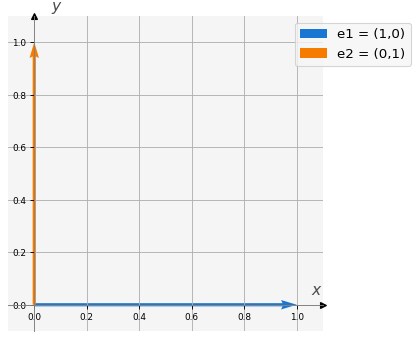
\includegraphics{03_CLineal_BOrtonormal_files/figure-pdf/cell-6-output-2.png}

Observa que los vectores \textbf{son ortogonales} y de tamaño unitario,
por lo que representan una base ortonormal de \(\mathbb{R}^2\).

Con esta base podemos representar cualquier vector de \(\mathbb{R}^2\),
particularmente \(\vec{x}_1 = (2, 3)\) y \(\vec{x}_2 = (3,1)\) del
\textbf{Ejemplo 1}.

\textbf{Construcción del vector \(\vec{x}_1\)}:

\begin{Shaded}
\begin{Highlighting}[]
\CommentTok{\# Construcción de la combinación lineal}
\NormalTok{z1 }\OperatorTok{=}\NormalTok{ x1[}\DecValTok{0}\NormalTok{] }\OperatorTok{*}\NormalTok{ e1 }
\NormalTok{z2 }\OperatorTok{=}\NormalTok{ x1[}\DecValTok{1}\NormalTok{] }\OperatorTok{*}\NormalTok{ e2}

\CommentTok{\# Resultado final}
\NormalTok{z }\OperatorTok{=}\NormalTok{ z1 }\OperatorTok{+}\NormalTok{ z2}

\CommentTok{\# Imprimimos el vector}
\BuiltInTok{print}\NormalTok{(}\StringTok{\textquotesingle{}x1 = }\SpecialCharTok{\{\}}\StringTok{\textquotesingle{}}\NormalTok{.}\BuiltInTok{format}\NormalTok{(z))}

\CommentTok{\# Visualizamos los vectores.}
\NormalTok{v }\OperatorTok{=}\NormalTok{ mvis.Plotter()  }\CommentTok{\# Definición de un objeto para crear figuras.}
\NormalTok{v.set\_coordsys(}\DecValTok{1}\NormalTok{)   }\CommentTok{\# Definición del sistema de coordenadas.}
\NormalTok{v.plot\_vectors\_sum(}\DecValTok{1}\NormalTok{, [z1, z2], [}\StringTok{\textquotesingle{}z1\textquotesingle{}}\NormalTok{, }\StringTok{\textquotesingle{}z2\textquotesingle{}}\NormalTok{],ofx}\OperatorTok{={-}}\FloatTok{0.2}\NormalTok{, w}\OperatorTok{=}\FloatTok{0.02}\NormalTok{) }\CommentTok{\# Graficación de los vectores \textquotesingle{}x\textquotesingle{} y \textquotesingle{}y\textquotesingle{}.}
\NormalTok{v.grid()  }\CommentTok{\# Muestra la rejilla del sistema de coordenadas.}
\end{Highlighting}
\end{Shaded}

\begin{verbatim}
x1 = [2 3]
\end{verbatim}

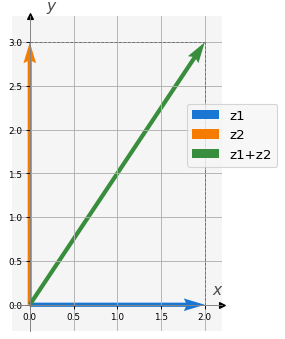
\includegraphics{03_CLineal_BOrtonormal_files/figure-pdf/cell-7-output-2.png}

\section{\texorpdfstring{\textbf{Ejercicio
1.}}{Ejercicio 1.}}\label{ejercicio-1.-2}

Construye \(\vec{x}_2\) usando la base ortonormal definida en el ejemplo
2 como se hizo para \(\vec{x}_1\).

\begin{Shaded}
\begin{Highlighting}[]
\CommentTok{\# Construcción de la combinación lineal}
\CommentTok{\# z1 = ...}
\CommentTok{\# z2 = ...}

\CommentTok{\# Resultado final}
\CommentTok{\# z = z1 + z2}

\CommentTok{\#\#\# }\RegionMarkerTok{BEGIN}\CommentTok{ SOLUTION}
\CommentTok{\# Construcción de la combinación lineal}
\NormalTok{z1 }\OperatorTok{=}\NormalTok{ x2[}\DecValTok{0}\NormalTok{] }\OperatorTok{*}\NormalTok{ e1}
\NormalTok{z2 }\OperatorTok{=}\NormalTok{ x2[}\DecValTok{1}\NormalTok{] }\OperatorTok{*}\NormalTok{ e2}

\CommentTok{\# Resultado final}
\NormalTok{z }\OperatorTok{=}\NormalTok{ z1 }\OperatorTok{+}\NormalTok{ z2}

\NormalTok{file\_answer }\OperatorTok{=}\NormalTok{FileAnswer()}
\NormalTok{file\_answer.write(}\StringTok{\textquotesingle{}1\textquotesingle{}}\NormalTok{, z, }\StringTok{\textquotesingle{}z es incorrecta: revisa la construcción de la combinación lineal.\textquotesingle{}}\NormalTok{)}
\CommentTok{\#\#\# }\RegionMarkerTok{END}\CommentTok{ SOLUTION}

\CommentTok{\# Imprimimos el vector}
\BuiltInTok{print}\NormalTok{(}\StringTok{\textquotesingle{}x2 = }\SpecialCharTok{\{\}}\StringTok{\textquotesingle{}}\NormalTok{.}\BuiltInTok{format}\NormalTok{(z))}

\CommentTok{\# Visualizamos los vectores.}
\NormalTok{v }\OperatorTok{=}\NormalTok{ mvis.Plotter()  }\CommentTok{\# Definición de un objeto para crear figuras.}
\NormalTok{v.set\_coordsys(}\DecValTok{1}\NormalTok{)   }\CommentTok{\# Definición del sistema de coordenadas.}
\NormalTok{v.plot\_vectors\_sum(}\DecValTok{1}\NormalTok{, [z1, z2], [}\StringTok{\textquotesingle{}z1\textquotesingle{}}\NormalTok{, }\StringTok{\textquotesingle{}z2\textquotesingle{}}\NormalTok{],ofx}\OperatorTok{={-}}\FloatTok{0.2}\NormalTok{, w}\OperatorTok{=}\FloatTok{0.0075}\NormalTok{) }\CommentTok{\# Graficación de los vectores \textquotesingle{}x\textquotesingle{} y \textquotesingle{}y\textquotesingle{}.}
\NormalTok{v.grid()  }\CommentTok{\# Muestra la rejilla del sistema de coordenadas.}
\end{Highlighting}
\end{Shaded}

\begin{verbatim}
Creando el directorio :/home/jovyan/macti/notebooks/.ans/Algebra_Lineal_01/
Respuestas y retroalimentación almacenadas.
x2 = [3 1]
\end{verbatim}

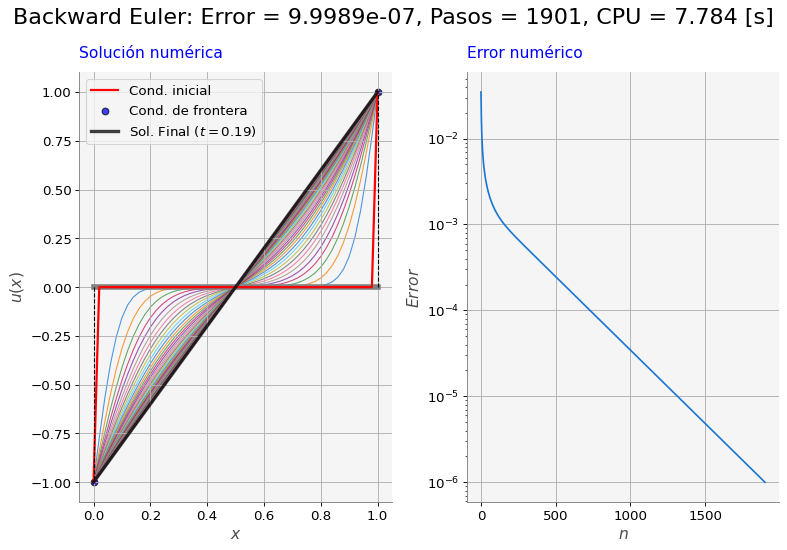
\includegraphics{03_CLineal_BOrtonormal_files/figure-pdf/cell-8-output-2.png}

\begin{Shaded}
\begin{Highlighting}[]
\NormalTok{quizz.eval\_numeric(}\StringTok{\textquotesingle{}1\textquotesingle{}}\NormalTok{, z)}
\end{Highlighting}
\end{Shaded}

\begin{verbatim}
----------------------------------------
1 | Tu resultado es correcto.
----------------------------------------
\end{verbatim}

\section{\texorpdfstring{\textbf{Ejercicio
2.}}{Ejercicio 2.}}\label{ejercicio-2.-1}

Usando \texttt{numpy} define la base ortonormal
\(\{\vec{e}_1, \vec{e}_2, \vec{e}_3, \vec{e}_4\} \in \mathbb{R}^4\) y
con ella construye el vector \(\vec{y} = (1.5, 1.0, 2.3, -1.0)\).
Imprime la base ortonormal y el resultado de construir el vector
\(\vec{y}\).

\begin{Shaded}
\begin{Highlighting}[]
\CommentTok{\#\#\# }\RegionMarkerTok{BEGIN}\CommentTok{ SOLUTION}
\NormalTok{e1 }\OperatorTok{=}\NormalTok{ np.array([}\DecValTok{1}\NormalTok{, }\DecValTok{0}\NormalTok{, }\DecValTok{0}\NormalTok{, }\DecValTok{0}\NormalTok{])}
\NormalTok{e2 }\OperatorTok{=}\NormalTok{ np.array([}\DecValTok{0}\NormalTok{, }\DecValTok{1}\NormalTok{, }\DecValTok{0}\NormalTok{, }\DecValTok{0}\NormalTok{])}
\NormalTok{e3 }\OperatorTok{=}\NormalTok{ np.array([}\DecValTok{0}\NormalTok{, }\DecValTok{0}\NormalTok{, }\DecValTok{1}\NormalTok{, }\DecValTok{0}\NormalTok{])}
\NormalTok{e4 }\OperatorTok{=}\NormalTok{ np.array([}\DecValTok{0}\NormalTok{, }\DecValTok{0}\NormalTok{, }\DecValTok{0}\NormalTok{, }\DecValTok{1}\NormalTok{])}

\CommentTok{\# Imprimimos los vectores}
\BuiltInTok{print}\NormalTok{(}\StringTok{\textquotesingle{}e1 = }\SpecialCharTok{\{\}}\StringTok{\textquotesingle{}}\NormalTok{.}\BuiltInTok{format}\NormalTok{(e1))}
\BuiltInTok{print}\NormalTok{(}\StringTok{\textquotesingle{}e2 = }\SpecialCharTok{\{\}}\StringTok{\textquotesingle{}}\NormalTok{.}\BuiltInTok{format}\NormalTok{(e2))}
\BuiltInTok{print}\NormalTok{(}\StringTok{\textquotesingle{}e3 = }\SpecialCharTok{\{\}}\StringTok{\textquotesingle{}}\NormalTok{.}\BuiltInTok{format}\NormalTok{(e3))}
\BuiltInTok{print}\NormalTok{(}\StringTok{\textquotesingle{}e4 = }\SpecialCharTok{\{\}}\StringTok{\textquotesingle{}}\NormalTok{.}\BuiltInTok{format}\NormalTok{(e4))}

\NormalTok{y1 }\OperatorTok{=} \FloatTok{1.5} \OperatorTok{*}\NormalTok{ e1}
\NormalTok{y2 }\OperatorTok{=} \FloatTok{1.0} \OperatorTok{*}\NormalTok{ e2}
\NormalTok{y3 }\OperatorTok{=} \FloatTok{2.3} \OperatorTok{*}\NormalTok{ e3}
\NormalTok{y4 }\OperatorTok{={-}}\FloatTok{1.0} \OperatorTok{*}\NormalTok{ e4}

\BuiltInTok{print}\NormalTok{(}\StringTok{\textquotesingle{} y = }\SpecialCharTok{\{\}}\StringTok{\textquotesingle{}}\NormalTok{.}\BuiltInTok{format}\NormalTok{(y1 }\OperatorTok{+}\NormalTok{ y2 }\OperatorTok{+}\NormalTok{ y3 }\OperatorTok{+}\NormalTok{ y4))}

\NormalTok{file\_answer.write(}\StringTok{\textquotesingle{}2\textquotesingle{}}\NormalTok{, e1, }\StringTok{\textquotesingle{}e1 es incorrecto: revisa la construcción del vector.\textquotesingle{}}\NormalTok{)}
\NormalTok{file\_answer.write(}\StringTok{\textquotesingle{}3\textquotesingle{}}\NormalTok{, e2, }\StringTok{\textquotesingle{}e2 es incorrecto: revisa la construcción del vector.\textquotesingle{}}\NormalTok{)}
\NormalTok{file\_answer.write(}\StringTok{\textquotesingle{}4\textquotesingle{}}\NormalTok{, e3, }\StringTok{\textquotesingle{}e3 es incorrecto: revisa la construcción del vector.\textquotesingle{}}\NormalTok{)}
\NormalTok{file\_answer.write(}\StringTok{\textquotesingle{}5\textquotesingle{}}\NormalTok{, e4, }\StringTok{\textquotesingle{}e4 es incorrecto: revisa la construcción del vector.\textquotesingle{}}\NormalTok{)}
\CommentTok{\#\#\# }\RegionMarkerTok{END}\CommentTok{ SOLUTION}
\end{Highlighting}
\end{Shaded}

\begin{verbatim}
e1 = [1 0 0 0]
e2 = [0 1 0 0]
e3 = [0 0 1 0]
e4 = [0 0 0 1]
 y = [ 1.5  1.   2.3 -1. ]
El directorio :/home/jovyan/macti/notebooks/.ans/Algebra_Lineal_01/ ya existe
Respuestas y retroalimentación almacenadas.
\end{verbatim}

\begin{Shaded}
\begin{Highlighting}[]
\NormalTok{quizz.eval\_numeric(}\StringTok{\textquotesingle{}2\textquotesingle{}}\NormalTok{, e1)}
\NormalTok{quizz.eval\_numeric(}\StringTok{\textquotesingle{}3\textquotesingle{}}\NormalTok{, e2)}
\NormalTok{quizz.eval\_numeric(}\StringTok{\textquotesingle{}4\textquotesingle{}}\NormalTok{, e3)}
\NormalTok{quizz.eval\_numeric(}\StringTok{\textquotesingle{}5\textquotesingle{}}\NormalTok{, e4)}
\end{Highlighting}
\end{Shaded}

\begin{verbatim}
----------------------------------------
2 | Tu resultado es correcto.
----------------------------------------
----------------------------------------
3 | Tu resultado es correcto.
----------------------------------------
----------------------------------------
4 | Tu resultado es correcto.
----------------------------------------
----------------------------------------
5 | Tu resultado es correcto.
----------------------------------------
\end{verbatim}

\bookmarksetup{startatroot}

\chapter{Normas vectoriales.}\label{normas-vectoriales.}

\textbf{Objetivo.}

Revisar e ilustrar los conceptos de normas vectoriales usando la
biblioteca \texttt{numpy}.

MACTI-Algebra\_Lineal\_01 by Luis M. de la Cruz is licensed under
Attribution-ShareAlike 4.0 International

Trabajo realizado con el apoyo del Programa UNAM-DGAPA-PAPIME PE101922

\begin{Shaded}
\begin{Highlighting}[]
\CommentTok{\# Importamos las bibliotecas requeridas}
\ImportTok{import}\NormalTok{ numpy }\ImportTok{as}\NormalTok{ np}
\ImportTok{import}\NormalTok{ ipywidgets }\ImportTok{as}\NormalTok{ widgets}
\ImportTok{import}\NormalTok{ macti.visual }\ImportTok{as}\NormalTok{ mvis}
\end{Highlighting}
\end{Shaded}

\bookmarksetup{startatroot}

\chapter{Definición.}\label{definiciuxf3n.}

Una función \(||\cdot ||\) de vectores se denomina norma vectorial si
para cualesquiera dos vectores \(\vec{x}\) y \(\vec{y}\) de
\(\mathbb{R}^n\) se satisfacen los siguiente axiomas:

\begin{enumerate}
\def\labelenumi{\arabic{enumi}.}
\tightlist
\item
  \(||\vec{x} || \ge 0\)
\item
  \(||\vec{x} || = 0 \iff \vec{x} = 0\)
\item
  \(||a\vec{x} || = |a| \; || \vec{x} ||\)
\item
  \(||\vec{x} + \vec{y}|| \le ||\vec{x} || + ||\vec{y}||\) (desigualdad
  triangular)
\end{enumerate}

\section{Tipos de normas.}\label{tipos-de-normas.}

\[
\begin{array}{lcl}
\text{Norma 1} & \rightarrow & ||\vec{x}||_1 = \sum_{i=1}^n |x_i|  \\
\text{Norma 2 (Euclideana)} & \rightarrow & ||\vec{x}||_2 = \left( \sum_{i=1}^n |x_i|^2 \right)^{1/2} = \langle \vec{x}, \vec{x} \rangle^{1/2} = (\vec{x}^T \cdot \vec{x})^{1/2}
\text{Norma 1} & \rightarrow & ||\vec{x}||_1 = \sum_{i=1}^n |x_i|  \\
\text{Norma Infinito} & \rightarrow & ||\vec{x}||_\infty = \max_{i \le 1 \le n} |x_i|
\end{array}
\]

\section{\texorpdfstring{\textbf{Ejemplo
1.}}{Ejemplo 1.}}\label{ejemplo-1.-1}

Para los vectores \(\vec{x} = (2, 3, -4, 5)\) y
\(\vec{y} = (3.0, -1.45, 8.5, 2.1)\) en \(\mathbb{R}^4\) probar que se
cumplen las propiedades de la norma para los tres tipos de norma antes
definidos.

Primero definimos los vectores

\begin{Shaded}
\begin{Highlighting}[]
\NormalTok{x }\OperatorTok{=}\NormalTok{ np.array([}\DecValTok{2}\NormalTok{, }\DecValTok{3}\NormalTok{, }\OperatorTok{{-}}\DecValTok{4}\NormalTok{, }\DecValTok{5}\NormalTok{]) }
\NormalTok{y }\OperatorTok{=}\NormalTok{ np.array([}\FloatTok{3.0}\NormalTok{, }\OperatorTok{{-}}\FloatTok{1.45}\NormalTok{, }\FloatTok{8.5}\NormalTok{, }\FloatTok{2.1}\NormalTok{])}

\CommentTok{\# Imprimimos los vectores}
\BuiltInTok{print}\NormalTok{(}\StringTok{\textquotesingle{}x = }\SpecialCharTok{\{\}}\StringTok{\textquotesingle{}}\NormalTok{.}\BuiltInTok{format}\NormalTok{(x))}
\BuiltInTok{print}\NormalTok{(}\StringTok{\textquotesingle{}y = }\SpecialCharTok{\{\}}\StringTok{\textquotesingle{}}\NormalTok{.}\BuiltInTok{format}\NormalTok{(y))}
\end{Highlighting}
\end{Shaded}

\begin{verbatim}
x = [ 2  3 -4  5]
y = [ 3.   -1.45  8.5   2.1 ]
\end{verbatim}

Podemos calcular los diferentes tipos de norma para estos vectores
usando la función \texttt{np.linalg.norm()}:

\begin{Shaded}
\begin{Highlighting}[]
\NormalTok{x\_n1 }\OperatorTok{=}\NormalTok{ np.linalg.norm(x, }\DecValTok{1}\NormalTok{)}
\NormalTok{y\_n1 }\OperatorTok{=}\NormalTok{ np.linalg.norm(y, }\DecValTok{1}\NormalTok{)}
\BuiltInTok{print}\NormalTok{(}\StringTok{\textquotesingle{}}\CharTok{\textbackslash{}n}\StringTok{Norma 1 }\CharTok{\textbackslash{}n}\StringTok{ ∥x∥₁ = }\SpecialCharTok{\{\}}\StringTok{ }\CharTok{\textbackslash{}n}\StringTok{ ∥y∥₁ = }\SpecialCharTok{\{\}}\StringTok{\textquotesingle{}}\NormalTok{.}\BuiltInTok{format}\NormalTok{(x\_n1, y\_n1))}

\NormalTok{x\_n2 }\OperatorTok{=}\NormalTok{ np.linalg.norm(x, }\DecValTok{2}\NormalTok{)}
\NormalTok{y\_n2 }\OperatorTok{=}\NormalTok{ np.linalg.norm(y, }\DecValTok{2}\NormalTok{)}
\BuiltInTok{print}\NormalTok{(}\StringTok{\textquotesingle{}}\CharTok{\textbackslash{}n}\StringTok{Norma 2 }\CharTok{\textbackslash{}n}\StringTok{ ∥x∥₂ = }\SpecialCharTok{\{\}}\StringTok{ }\CharTok{\textbackslash{}n}\StringTok{ ∥y∥₂ = }\SpecialCharTok{\{\}}\StringTok{\textquotesingle{}}\NormalTok{.}\BuiltInTok{format}\NormalTok{(x\_n2, y\_n2))}

\NormalTok{x\_nI }\OperatorTok{=}\NormalTok{ np.linalg.norm(x, np.infty)}
\NormalTok{y\_nI }\OperatorTok{=}\NormalTok{ np.linalg.norm(y, np.infty)}
\BuiltInTok{print}\NormalTok{(}\StringTok{\textquotesingle{}}\CharTok{\textbackslash{}n}\StringTok{Norma infinito }\CharTok{\textbackslash{}n}\StringTok{ ∥x∥∞ = }\SpecialCharTok{\{\}}\StringTok{ }\CharTok{\textbackslash{}n}\StringTok{ ∥y∥∞ = }\SpecialCharTok{\{\}}\StringTok{\textquotesingle{}}\NormalTok{.}\BuiltInTok{format}\NormalTok{(x\_nI, y\_nI))}
\end{Highlighting}
\end{Shaded}

\begin{verbatim}

Norma 1 
 ∥x∥₁ = 14.0 
 ∥y∥₁ = 15.049999999999999

Norma 2 
 ∥x∥₂ = 7.3484692283495345 
 ∥y∥₂ = 9.368164174479437

Norma infinito 
 ∥x∥∞ = 5.0 
 ∥y∥∞ = 8.5
\end{verbatim}

\textbf{Propiedad 1}: Del resultado observamos que en todos los casos la
norma es mayor que \(0\).

\textbf{Propiedad 2}: En ningún caso la norma es igual a \(0\), pues
tanto \(\vec{x}\) como \(\vec{y}\) son diferentes de cero. La norma solo
será igual a \(0\) si el vector es idénticamente \(0\):

\begin{Shaded}
\begin{Highlighting}[]
\NormalTok{z }\OperatorTok{=}\NormalTok{ np.zeros(}\DecValTok{4}\NormalTok{)}
\BuiltInTok{print}\NormalTok{(}\StringTok{\textquotesingle{}z = }\SpecialCharTok{\{\}}\StringTok{\textquotesingle{}}\NormalTok{.}\BuiltInTok{format}\NormalTok{(z))}

\NormalTok{z\_n1 }\OperatorTok{=}\NormalTok{ np.linalg.norm(z, }\DecValTok{1}\NormalTok{)}
\BuiltInTok{print}\NormalTok{(}\StringTok{\textquotesingle{}}\CharTok{\textbackslash{}n}\StringTok{Norma 1 }\CharTok{\textbackslash{}n}\StringTok{ ∥z∥₁ = }\SpecialCharTok{\{\}}\StringTok{\textquotesingle{}}\NormalTok{.}\BuiltInTok{format}\NormalTok{(z\_n1))}

\NormalTok{z\_n2 }\OperatorTok{=}\NormalTok{ np.linalg.norm(z, }\DecValTok{2}\NormalTok{)}
\BuiltInTok{print}\NormalTok{(}\StringTok{\textquotesingle{}}\CharTok{\textbackslash{}n}\StringTok{Norma 2 }\CharTok{\textbackslash{}n}\StringTok{ ∥z∥₂ = }\SpecialCharTok{\{\}}\StringTok{\textquotesingle{}}\NormalTok{.}\BuiltInTok{format}\NormalTok{(z\_n2))}

\NormalTok{z\_nI }\OperatorTok{=}\NormalTok{ np.linalg.norm(z, np.infty)}
\BuiltInTok{print}\NormalTok{(}\StringTok{\textquotesingle{}}\CharTok{\textbackslash{}n}\StringTok{Norma infinito }\CharTok{\textbackslash{}n}\StringTok{ ∥z∥∞ = }\SpecialCharTok{\{\}}\StringTok{\textquotesingle{}}\NormalTok{.}\BuiltInTok{format}\NormalTok{(z\_nI))}
\end{Highlighting}
\end{Shaded}

\begin{verbatim}
z = [0. 0. 0. 0.]

Norma 1 
 ∥z∥₁ = 0.0

Norma 2 
 ∥z∥₂ = 0.0

Norma infinito 
 ∥z∥∞ = 0.0
\end{verbatim}

\textbf{Propiedad 3}: definimos un escalar \(a = -3.5\) entonces:

\begin{Shaded}
\begin{Highlighting}[]
\NormalTok{a }\OperatorTok{=} \OperatorTok{{-}}\FloatTok{3.5}
\BuiltInTok{print}\NormalTok{(}\StringTok{\textquotesingle{}a = }\SpecialCharTok{\{\}}\StringTok{, }\CharTok{\textbackslash{}t}\StringTok{ x = }\SpecialCharTok{\{\}}\StringTok{\textquotesingle{}}\NormalTok{.}\BuiltInTok{format}\NormalTok{(a, x))}
      
\NormalTok{a\_x\_n1 }\OperatorTok{=}\NormalTok{ np.linalg.norm(a }\OperatorTok{*}\NormalTok{ x, }\DecValTok{1}\NormalTok{) }
\NormalTok{a\_x\_n2 }\OperatorTok{=}\NormalTok{ np.linalg.norm(a }\OperatorTok{*}\NormalTok{ x, }\DecValTok{2}\NormalTok{) }
\NormalTok{a\_x\_nI }\OperatorTok{=}\NormalTok{ np.linalg.norm(a }\OperatorTok{*}\NormalTok{ x, np.infty) }

\BuiltInTok{print}\NormalTok{(}\StringTok{\textquotesingle{}}\CharTok{\textbackslash{}n}\StringTok{ ∥a x∥₁ = }\SpecialCharTok{\{\}}\StringTok{ }\CharTok{\textbackslash{}n}\StringTok{ |a| ∥x∥₁ = }\SpecialCharTok{\{\}}\StringTok{\textquotesingle{}}\NormalTok{.}\BuiltInTok{format}\NormalTok{(a\_x\_n1, np.}\BuiltInTok{abs}\NormalTok{(a) }\OperatorTok{*}\NormalTok{ x\_n1))}
\BuiltInTok{print}\NormalTok{(}\StringTok{\textquotesingle{}}\CharTok{\textbackslash{}n}\StringTok{ ∥a x∥₂ = }\SpecialCharTok{\{\}}\StringTok{ }\CharTok{\textbackslash{}n}\StringTok{ |a| ∥x∥₂ = }\SpecialCharTok{\{\}}\StringTok{\textquotesingle{}}\NormalTok{.}\BuiltInTok{format}\NormalTok{(a\_x\_n2, np.}\BuiltInTok{abs}\NormalTok{(a) }\OperatorTok{*}\NormalTok{ x\_n2))}
\BuiltInTok{print}\NormalTok{(}\StringTok{\textquotesingle{}}\CharTok{\textbackslash{}n}\StringTok{ ∥a x∥∞ = }\SpecialCharTok{\{\}}\StringTok{ }\CharTok{\textbackslash{}n}\StringTok{ |a| ∥x∥∞ = }\SpecialCharTok{\{\}}\StringTok{\textquotesingle{}}\NormalTok{.}\BuiltInTok{format}\NormalTok{(a\_x\_nI, np.}\BuiltInTok{abs}\NormalTok{(a) }\OperatorTok{*}\NormalTok{ x\_nI))}
\end{Highlighting}
\end{Shaded}

\begin{verbatim}
a = -3.5,    x = [ 2  3 -4  5]

 ∥a x∥₁ = 49.0 
 |a| ∥x∥₁ = 49.0

 ∥a x∥₂ = 25.71964229922337 
 |a| ∥x∥₂ = 25.71964229922337

 ∥a x∥∞ = 17.5 
 |a| ∥x∥∞ = 17.5
\end{verbatim}

\textbf{Propiedad 4}:

\begin{Shaded}
\begin{Highlighting}[]
\NormalTok{x\_p\_y\_n1 }\OperatorTok{=}\NormalTok{ np.linalg.norm(x}\OperatorTok{+}\NormalTok{y, }\DecValTok{1}\NormalTok{)}
\BuiltInTok{print}\NormalTok{(}\StringTok{\textquotesingle{}}\CharTok{\textbackslash{}n}\StringTok{Norma 1:\textquotesingle{}}\NormalTok{)}
\BuiltInTok{print}\NormalTok{(}\StringTok{\textquotesingle{} ∥x + y∥₁ = }\SpecialCharTok{\{\}}\StringTok{\textquotesingle{}}\NormalTok{.}\BuiltInTok{format}\NormalTok{(x\_p\_y\_n1))}
\BuiltInTok{print}\NormalTok{(}\StringTok{\textquotesingle{} ∥x∥₁ + ∥y∥₁ = }\SpecialCharTok{\{\}}\StringTok{\textquotesingle{}}\NormalTok{.}\BuiltInTok{format}\NormalTok{(x\_n1 }\OperatorTok{+}\NormalTok{ y\_n1))}
\BuiltInTok{print}\NormalTok{(}\StringTok{\textquotesingle{} ¿ ∥x + y∥₁ ≤ ∥x∥₁ + ∥y∥₁ ? : }\SpecialCharTok{\{\}}\StringTok{\textquotesingle{}}\NormalTok{.}\BuiltInTok{format}\NormalTok{(x\_p\_y\_n1 }\OperatorTok{\textless{}=}\NormalTok{ x\_n1 }\OperatorTok{+}\NormalTok{ y\_n1))}
\end{Highlighting}
\end{Shaded}

\begin{verbatim}

Norma 1:
 ∥x + y∥₁ = 18.15
 ∥x∥₁ + ∥y∥₁ = 29.049999999999997
 ¿ ∥x + y∥₁ ≤ ∥x∥₁ + ∥y∥₁ ? : True
\end{verbatim}

\section{\texorpdfstring{\textbf{Ejercicio
1.}}{Ejercicio 1.}}\label{ejercicio-1.-3}

Verifica que la propiedad 4 se cumple para las normas 2 e infinito para
los vectores \(\vec{x}\) y \(\vec{y}\) antes defnidos.

El resultado debería ser:

\begin{verbatim}
Norma 2:
 ∥x + y∥₂ = 9.90265116016918
 ∥x∥₂ + ∥y∥₂ = 16.716633402828972
 ¿ ∥x + y∥₂ ≤ ∥x∥₂ + ∥y∥₂ ? : True

Norma Infinito:
 ∥x + y∥∞ = 7.1
 ∥x∥∞ + ∥y∥∞ = 13.5
 ¿ ∥x + y∥∞ ≤ ∥x∥∞ + ∥y∥∞ ? : True
\end{verbatim}

\begin{Shaded}
\begin{Highlighting}[]
\CommentTok{\#\#\# }\RegionMarkerTok{BEGIN}\CommentTok{ SOLUTION}
\NormalTok{x\_p\_y\_n2 }\OperatorTok{=}\NormalTok{ np.linalg.norm(x}\OperatorTok{+}\NormalTok{y, }\DecValTok{2}\NormalTok{)}
\BuiltInTok{print}\NormalTok{(}\StringTok{\textquotesingle{}}\CharTok{\textbackslash{}n}\StringTok{Norma 2:\textquotesingle{}}\NormalTok{)}
\BuiltInTok{print}\NormalTok{(}\StringTok{\textquotesingle{} ∥x + y∥₂ = }\SpecialCharTok{\{\}}\StringTok{\textquotesingle{}}\NormalTok{.}\BuiltInTok{format}\NormalTok{(x\_p\_y\_n2))}
\BuiltInTok{print}\NormalTok{(}\StringTok{\textquotesingle{} ∥x∥₂ + ∥y∥₂ = }\SpecialCharTok{\{\}}\StringTok{\textquotesingle{}}\NormalTok{.}\BuiltInTok{format}\NormalTok{(x\_n2 }\OperatorTok{+}\NormalTok{ y\_n2))}
\BuiltInTok{print}\NormalTok{(}\StringTok{\textquotesingle{} ¿ ∥x + y∥₂ ≤ ∥x∥₂ + ∥y∥₂ ? : }\SpecialCharTok{\{\}}\StringTok{\textquotesingle{}}\NormalTok{.}\BuiltInTok{format}\NormalTok{(x\_p\_y\_n2 }\OperatorTok{\textless{}=}\NormalTok{ x\_n2 }\OperatorTok{+}\NormalTok{ y\_n2))}


\NormalTok{x\_p\_y\_nI }\OperatorTok{=}\NormalTok{ np.linalg.norm(x}\OperatorTok{+}\NormalTok{y, np.infty)}
\BuiltInTok{print}\NormalTok{(}\StringTok{\textquotesingle{}}\CharTok{\textbackslash{}n}\StringTok{Norma Infinito:\textquotesingle{}}\NormalTok{)}
\BuiltInTok{print}\NormalTok{(}\StringTok{\textquotesingle{} ∥x + y∥∞ = }\SpecialCharTok{\{\}}\StringTok{\textquotesingle{}}\NormalTok{.}\BuiltInTok{format}\NormalTok{(x\_p\_y\_nI))}
\BuiltInTok{print}\NormalTok{(}\StringTok{\textquotesingle{} ∥x∥∞ + ∥y∥∞ = }\SpecialCharTok{\{\}}\StringTok{\textquotesingle{}}\NormalTok{.}\BuiltInTok{format}\NormalTok{(x\_nI }\OperatorTok{+}\NormalTok{ y\_nI))}
\BuiltInTok{print}\NormalTok{(}\StringTok{\textquotesingle{} ¿ ∥x + y∥∞ ≤ ∥x∥∞ + ∥y∥∞ ? : }\SpecialCharTok{\{\}}\StringTok{\textquotesingle{}}\NormalTok{.}\BuiltInTok{format}\NormalTok{(x\_p\_y\_nI }\OperatorTok{\textless{}=}\NormalTok{ x\_nI }\OperatorTok{+}\NormalTok{ y\_nI))}
\CommentTok{\#\#\# }\RegionMarkerTok{END}\CommentTok{ SOLUTION}
\end{Highlighting}
\end{Shaded}

\begin{verbatim}

Norma 2:
 ∥x + y∥₂ = 9.90265116016918
 ∥x∥₂ + ∥y∥₂ = 16.716633402828972
 ¿ ∥x + y∥₂ ≤ ∥x∥₂ + ∥y∥₂ ? : True

Norma Infinito:
 ∥x + y∥∞ = 7.1
 ∥x∥∞ + ∥y∥∞ = 13.5
 ¿ ∥x + y∥∞ ≤ ∥x∥∞ + ∥y∥∞ ? : True
\end{verbatim}

\section{Desigualdad de Holder.}\label{desigualdad-de-holder.}

Para cualesquiera dos vectores \(\vec{x}\), \(\vec{y}\) se cumple: \[
|\vec{x}^T \cdot \vec{y}| \le ||\vec{x}||_p ||\vec{y}||_q, \,\,\, \mbox{donde}
\,\,\, p > 1, q > 1 \,\,\, \mbox{y} \;\; \frac{1}{p} + \frac{1}{q} = 1
\] (Cuando \(p = q = 2\) se obtiene la desigualdad de Schwarz)

\section{\texorpdfstring{\textbf{Ejercicio
2.}}{Ejercicio 2.}}\label{ejercicio-2.-2}

Verifica que se cumple la desigualdad de Schwarz para los vectores
\(\vec{x}\) y \(\vec{y}\) antes definidos.

El resultado debería ser:

\begin{verbatim}
Desigualdad de Holder
 |<x, y>| = 21.85
 ∥x∥p * ∥y∥q = 68.84166616228866
 ¿ |<x, y>| ≤ ∥x∥p * ∥y∥q ? : True
\end{verbatim}

\begin{Shaded}
\begin{Highlighting}[]
\CommentTok{\#\#\# }\RegionMarkerTok{BEGIN}\CommentTok{ SOLUTION}
\BuiltInTok{print}\NormalTok{(}\StringTok{\textquotesingle{}}\CharTok{\textbackslash{}n}\StringTok{Desigualdad de Holder\textquotesingle{}}\NormalTok{)}
\NormalTok{x\_dot\_y }\OperatorTok{=}\NormalTok{ np.}\BuiltInTok{abs}\NormalTok{(np.dot(x, y))}

\BuiltInTok{print}\NormalTok{(}\StringTok{\textquotesingle{} |\textless{}x, y\textgreater{}| = }\SpecialCharTok{\{\}}\StringTok{\textquotesingle{}}\NormalTok{.}\BuiltInTok{format}\NormalTok{(x\_dot\_y))}
\BuiltInTok{print}\NormalTok{(}\StringTok{\textquotesingle{} ∥x∥p * ∥y∥q = }\SpecialCharTok{\{\}}\StringTok{\textquotesingle{}}\NormalTok{.}\BuiltInTok{format}\NormalTok{(x\_n2 }\OperatorTok{*}\NormalTok{ y\_n2))}
\BuiltInTok{print}\NormalTok{(}\StringTok{\textquotesingle{} ¿ |\textless{}x, y\textgreater{}| ≤ ∥x∥p * ∥y∥q ? : }\SpecialCharTok{\{\}}\StringTok{\textquotesingle{}}\NormalTok{.}\BuiltInTok{format}\NormalTok{(x\_dot\_y }\OperatorTok{\textless{}=}\NormalTok{ x\_n2 }\OperatorTok{*}\NormalTok{ y\_n2))}
\CommentTok{\#\#\# }\RegionMarkerTok{END}\CommentTok{ SOLUTION}
\end{Highlighting}
\end{Shaded}

\begin{verbatim}

Desigualdad de Holder
 |<x, y>| = 21.85
 ∥x∥p * ∥y∥q = 68.84166616228866
 ¿ |<x, y>| ≤ ∥x∥p * ∥y∥q ? : True
\end{verbatim}

\section{Equivalencia de normas.}\label{equivalencia-de-normas.}

En un espacio \(\mathbb{R}^n\) de dimensi\textquotesingle on finita,
cualquiera dos normas arbitrarias son equivalentes:

\[
\begin{eqnarray*}
||\vec{x}||_2 \le & ||\vec{x}||_1 & \le \sqrt{n} ||x||_2 \\
||\vec{x}||_\infty \le & ||\vec{x}||_2 & \le \sqrt{n} ||x||_\infty \\
||\vec{x}||_\infty \le & ||\vec{x}||_1 & \le n ||x||_\infty
\end{eqnarray*}
\]

\begin{Shaded}
\begin{Highlighting}[]
\BuiltInTok{print}\NormalTok{(}\StringTok{\textquotesingle{}}\CharTok{\textbackslash{}n}\StringTok{Equivalencia entre norma 1 y norma 2}\CharTok{\textbackslash{}n}\StringTok{\textquotesingle{}}\NormalTok{)}
\BuiltInTok{print}\NormalTok{(}\StringTok{\textquotesingle{}∥x∥₂ = }\SpecialCharTok{\{\}}\StringTok{, ∥x∥₁ = }\SpecialCharTok{\{\}}\StringTok{, √4 * ∥x∥₂ = }\SpecialCharTok{\{\}}\StringTok{ }\CharTok{\textbackslash{}n}\StringTok{\textquotesingle{}}\NormalTok{.}\BuiltInTok{format}\NormalTok{(x\_n2, x\_n1, np.sqrt(}\DecValTok{4}\NormalTok{) }\OperatorTok{*}\NormalTok{ x\_n2))}
\BuiltInTok{print}\NormalTok{(}\StringTok{\textquotesingle{}¿ ∥x∥₂ ≤ ∥x∥₁ ≤ √4 * ∥x∥₂ ? : }\SpecialCharTok{\{\}}\StringTok{\textquotesingle{}}\NormalTok{.}\BuiltInTok{format}\NormalTok{(x\_n2 }\OperatorTok{\textless{}=}\NormalTok{ x\_n1 }\OperatorTok{\textless{}=}\NormalTok{ np.sqrt(}\DecValTok{4}\NormalTok{) }\OperatorTok{*}\NormalTok{ x\_n2))}
\end{Highlighting}
\end{Shaded}

\begin{verbatim}

Equivalencia entre norma 1 y norma 2

∥x∥₂ = 7.3484692283495345, ∥x∥₁ = 14.0, √4 * ∥x∥₂ = 14.696938456699069 

¿ ∥x∥₂ ≤ ∥x∥₁ ≤ √4 * ∥x∥₂ ? : True
\end{verbatim}

\section{\texorpdfstring{\textbf{Ejercicio
3.}}{Ejercicio 3.}}\label{ejercicio-3.}

Verificar la equivalencia entre las normas \(||\cdot||_\infty\) y
\(||\cdot||_2\) y entre \(||\cdot||_\infty\) y \(||\cdot||_1\) para los
vectores \(\vec{x}\) y \(\vec{y}\) antes definidos.

El resultado debería ser:

\begin{verbatim}
Equivalencia entre norma infinito y norma 2

∥x∥∞ = 5.0, ∥x∥₂ = 7.3484692283495345, √n * ∥x∥∞ = 10.0

¿ ∥x∥∞ ≤ ∥x∥₂ ≤ √n * ∥x∥∞ ? : True

Equivalencia entre norma infinito y norma 1

∥x∥∞ = 5.0, ∥x∥₁ = 14.0, n * ∥x∥∞ = 20.0

¿ ∥x∥∞ ≤ ∥x∥₁ ≤ n * ∥x∥∞ ? : True
\end{verbatim}

\begin{Shaded}
\begin{Highlighting}[]
\CommentTok{\#\#\# }\RegionMarkerTok{BEGIN}\CommentTok{ SOLUTION}
\NormalTok{n }\OperatorTok{=} \DecValTok{4}
\BuiltInTok{print}\NormalTok{(}\StringTok{\textquotesingle{}}\CharTok{\textbackslash{}n}\StringTok{Equivalencia entre norma infinito y norma 2}\CharTok{\textbackslash{}n}\StringTok{\textquotesingle{}}\NormalTok{)}
\BuiltInTok{print}\NormalTok{(}\StringTok{\textquotesingle{}∥x∥∞ = }\SpecialCharTok{\{\}}\StringTok{, ∥x∥₂ = }\SpecialCharTok{\{\}}\StringTok{, √n * ∥x∥∞ = }\SpecialCharTok{\{\}}\CharTok{\textbackslash{}n}\StringTok{\textquotesingle{}}\NormalTok{.}\BuiltInTok{format}\NormalTok{(x\_nI, x\_n2, np.sqrt(n) }\OperatorTok{*}\NormalTok{ x\_nI))}
\BuiltInTok{print}\NormalTok{(}\StringTok{\textquotesingle{}¿ ∥x∥∞ ≤ ∥x∥₂ ≤ √n * ∥x∥∞ ? : }\SpecialCharTok{\{\}}\StringTok{\textquotesingle{}}\NormalTok{.}\BuiltInTok{format}\NormalTok{(x\_nI }\OperatorTok{\textless{}=}\NormalTok{ x\_n2 }\OperatorTok{\textless{}=}\NormalTok{ np.sqrt(n) }\OperatorTok{*}\NormalTok{ x\_nI))}

\BuiltInTok{print}\NormalTok{(}\StringTok{\textquotesingle{}}\CharTok{\textbackslash{}n}\StringTok{Equivalencia entre norma infinito y norma 1}\CharTok{\textbackslash{}n}\StringTok{\textquotesingle{}}\NormalTok{)}
\BuiltInTok{print}\NormalTok{(}\StringTok{\textquotesingle{}∥x∥∞ = }\SpecialCharTok{\{\}}\StringTok{, ∥x∥₁ = }\SpecialCharTok{\{\}}\StringTok{, n * ∥x∥∞ = }\SpecialCharTok{\{\}}\CharTok{\textbackslash{}n}\StringTok{\textquotesingle{}}\NormalTok{.}\BuiltInTok{format}\NormalTok{(x\_nI, x\_n1, n }\OperatorTok{*}\NormalTok{ x\_nI))}
\BuiltInTok{print}\NormalTok{(}\StringTok{\textquotesingle{}¿ ∥x∥∞ ≤ ∥x∥₁ ≤ n * ∥x∥∞ ? : }\SpecialCharTok{\{\}}\StringTok{\textquotesingle{}}\NormalTok{.}\BuiltInTok{format}\NormalTok{(x\_nI }\OperatorTok{\textless{}=}\NormalTok{ x\_n1 }\OperatorTok{\textless{}=}\NormalTok{ n }\OperatorTok{*}\NormalTok{ x\_nI))}
\CommentTok{\#\#\# }\RegionMarkerTok{END}\CommentTok{ SOLUTION}
\end{Highlighting}
\end{Shaded}

\begin{verbatim}

Equivalencia entre norma infinito y norma 2

∥x∥∞ = 5.0, ∥x∥₂ = 7.3484692283495345, √n * ∥x∥∞ = 10.0

¿ ∥x∥∞ ≤ ∥x∥₂ ≤ √n * ∥x∥∞ ? : True

Equivalencia entre norma infinito y norma 1

∥x∥∞ = 5.0, ∥x∥₁ = 14.0, n * ∥x∥∞ = 20.0

¿ ∥x∥∞ ≤ ∥x∥₁ ≤ n * ∥x∥∞ ? : True
\end{verbatim}

\bookmarksetup{startatroot}

\chapter{Matrices, normas y
eigenvalores/eigenvectores.}\label{matrices-normas-y-eigenvaloreseigenvectores.}

\textbf{Objetivo.}

Revisar e ilustrar los conceptos de matrices, sus normas y
eigenvalores/eigenvectores usando la biblioteca \texttt{numpy}.

MACTI-Algebra\_Lineal\_01 by Luis M. de la Cruz is licensed under
Attribution-ShareAlike 4.0 International

Trabajo realizado con el apoyo del Programa UNAM-DGAPA-PAPIME PE101922

\begin{Shaded}
\begin{Highlighting}[]
\CommentTok{\# Importamos las bibliotecas requeridas}
\ImportTok{import}\NormalTok{ numpy }\ImportTok{as}\NormalTok{ np}
\ImportTok{import}\NormalTok{ sympy}
\ImportTok{import}\NormalTok{ ipywidgets }\ImportTok{as}\NormalTok{ widgets}
\ImportTok{import}\NormalTok{ macti.visual }\ImportTok{as}\NormalTok{ mvis}
\ImportTok{import}\NormalTok{ macti.matem }\ImportTok{as}\NormalTok{ mmat}
\end{Highlighting}
\end{Shaded}

Sea \(A = a_{ij}\) una matriz de \(n \times n\), donde \(n\) indica la
dimensión de la matriz (\(n\) renglones por \(n\) columnas). Los números
\(a_{ij}\) son los elementos de la matriz, y \(i,j = 1,\dots,n\). La
matriz \(A^T = {a_{ji}}\) es la matriz transpuesta.

\[
A = 
\left(
\begin{array}{cccc}
a_{11} & a_{12} & \dots & a_{1n}\\
a_{21} & a_{22} & \dots & a_{2n}\\
\vdots & \vdots& \ddots & \vdots \\
a_{n1} & a_{n2} & \dots & a_{nn}\\
\end{array}
\right)
\,\,\,\,
A^T = 
\left(
\begin{array}{cccc}
a_{11} & a_{21} & \dots & a_{n1}\\
a_{12} & a_{22} & \dots & a_{n2}\\
\vdots & \vdots& \ddots & \vdots \\
a_{1n} & a_{2n} & \dots & a_{nn}\\
\end{array}
\right)
\]

Definamos una matriz usando \texttt{numpy}:

\begin{Shaded}
\begin{Highlighting}[]
\NormalTok{A }\OperatorTok{=}\NormalTok{ np.array([[}\DecValTok{2}\NormalTok{, }\DecValTok{3}\NormalTok{, }\DecValTok{5}\NormalTok{],}
\NormalTok{              [}\DecValTok{1}\NormalTok{, }\OperatorTok{{-}}\DecValTok{4}\NormalTok{, }\DecValTok{8}\NormalTok{],}
\NormalTok{              [}\DecValTok{8}\NormalTok{, }\DecValTok{6}\NormalTok{, }\DecValTok{3}\NormalTok{]])}
\NormalTok{A}
\end{Highlighting}
\end{Shaded}

\begin{verbatim}
array([[ 2,  3,  5],
       [ 1, -4,  8],
       [ 8,  6,  3]])
\end{verbatim}

\section{Matriz transpuesta}\label{matriz-transpuesta}

La matriz \(A^T = {a_{ji}}\) es la matriz transpuesta.

\begin{Shaded}
\begin{Highlighting}[]
\NormalTok{AT }\OperatorTok{=}\NormalTok{ A.T}
\NormalTok{AT}
\end{Highlighting}
\end{Shaded}

\begin{verbatim}
array([[ 2,  1,  8],
       [ 3, -4,  6],
       [ 5,  8,  3]])
\end{verbatim}

\section{Matriz identidad}\label{matriz-identidad}

La matriz identidad \(I\) es aquella donde todas sus entradas son cero
excepto en la diagonal donde sus entradas son 1.

\begin{Shaded}
\begin{Highlighting}[]
\NormalTok{I }\OperatorTok{=}\NormalTok{ np.eye(}\DecValTok{3}\NormalTok{)}
\NormalTok{I}
\end{Highlighting}
\end{Shaded}

\begin{verbatim}
array([[1., 0., 0.],
       [0., 1., 0.],
       [0., 0., 1.]])
\end{verbatim}

\section{Matriz inversa}\label{matriz-inversa}

La matriz inversa de \(A\) se denota por \(A^{-1}\) y es tal que
\(A^{-1}A = I\).

\begin{Shaded}
\begin{Highlighting}[]
\NormalTok{Ainv }\OperatorTok{=}\NormalTok{ np.linalg.inv(A)}
\NormalTok{Ainv}
\end{Highlighting}
\end{Shaded}

\begin{verbatim}
array([[-0.23715415,  0.08300395,  0.17391304],
       [ 0.24110672, -0.13438735, -0.04347826],
       [ 0.15019763,  0.04743083, -0.04347826]])
\end{verbatim}

\begin{Shaded}
\begin{Highlighting}[]
\CommentTok{\# Comprobar que Ainv es la inversa de A}
\NormalTok{np.dot(A, Ainv)}
\end{Highlighting}
\end{Shaded}

\begin{verbatim}
array([[1.00000000e+00, 0.00000000e+00, 2.77555756e-17],
       [2.22044605e-16, 1.00000000e+00, 0.00000000e+00],
       [1.11022302e-16, 2.77555756e-17, 1.00000000e+00]])
\end{verbatim}

\section{Matriz diagonal}\label{matriz-diagonal}

Una matriz \(A = {a_{ij}}\) se llama diagonal si
\(a_{ij}=0, \forall i \ne j\) y se denota por \(A = \mbox{diag}\)
\({a_{ii}}\).

\begin{Shaded}
\begin{Highlighting}[]
\NormalTok{A}
\end{Highlighting}
\end{Shaded}

\begin{verbatim}
array([[ 2,  3,  5],
       [ 1, -4,  8],
       [ 8,  6,  3]])
\end{verbatim}

\begin{Shaded}
\begin{Highlighting}[]
\NormalTok{np.diagonal(A)}
\end{Highlighting}
\end{Shaded}

\begin{verbatim}
array([ 2, -4,  3])
\end{verbatim}

\begin{Shaded}
\begin{Highlighting}[]
\CommentTok{\# Diagonales inferiores}
\NormalTok{np.diagonal(A,}\DecValTok{1}\NormalTok{)}
\end{Highlighting}
\end{Shaded}

\begin{verbatim}
array([3, 8])
\end{verbatim}

\begin{Shaded}
\begin{Highlighting}[]
\CommentTok{\# Diagonales superiores}
\NormalTok{np.diagonal(A,}\OperatorTok{{-}}\DecValTok{1}\NormalTok{)}
\end{Highlighting}
\end{Shaded}

\begin{verbatim}
array([1, 6])
\end{verbatim}

\section{Matriz triangular superior e
inferior}\label{matriz-triangular-superior-e-inferior}

Una matriz \(A = {a_{ij}}\) se llama triangular superior si
\(a_{ij} = 0, \forall i > j\) y triangular inferior si
\(a_{ij} = 0, \forall i < j\).

\begin{Shaded}
\begin{Highlighting}[]
\CommentTok{\# Matriz triangular superior}
\NormalTok{np.triu(A)}
\end{Highlighting}
\end{Shaded}

\begin{verbatim}
array([[ 2,  3,  5],
       [ 0, -4,  8],
       [ 0,  0,  3]])
\end{verbatim}

\begin{Shaded}
\begin{Highlighting}[]
\CommentTok{\# Matriz triangular inferior}
\NormalTok{np.tril(A)}
\end{Highlighting}
\end{Shaded}

\begin{verbatim}
array([[ 2,  0,  0],
       [ 1, -4,  0],
       [ 8,  6,  3]])
\end{verbatim}

\section{Matrices simétricas}\label{matrices-simuxe9tricas}

Una matriz \(A\) es simétrica si \(A^T = A\) y antisimétrica si
\(A^T = -A\).

\begin{Shaded}
\begin{Highlighting}[]
\NormalTok{B }\OperatorTok{=}\NormalTok{ np.array([[}\DecValTok{2}\NormalTok{, }\DecValTok{3}\NormalTok{, }\DecValTok{5}\NormalTok{],}
\NormalTok{              [}\DecValTok{3}\NormalTok{, }\OperatorTok{{-}}\DecValTok{4}\NormalTok{, }\DecValTok{8}\NormalTok{],}
\NormalTok{              [}\DecValTok{5}\NormalTok{, }\DecValTok{8}\NormalTok{, }\DecValTok{3}\NormalTok{]])}
\end{Highlighting}
\end{Shaded}

\begin{Shaded}
\begin{Highlighting}[]
\BuiltInTok{print}\NormalTok{(}\StringTok{\textquotesingle{}Matriz A = }\CharTok{\textbackslash{}n}\SpecialCharTok{\{\}}\StringTok{ }\CharTok{\textbackslash{}n\textbackslash{}n}\StringTok{Matriz B = }\CharTok{\textbackslash{}n}\SpecialCharTok{\{\}}\StringTok{\textquotesingle{}}\NormalTok{.}\BuiltInTok{format}\NormalTok{(A,B))}
\end{Highlighting}
\end{Shaded}

\begin{verbatim}
Matriz A = 
[[ 2  3  5]
 [ 1 -4  8]
 [ 8  6  3]] 

Matriz B = 
[[ 2  3  5]
 [ 3 -4  8]
 [ 5  8  3]]
\end{verbatim}

\begin{Shaded}
\begin{Highlighting}[]
\CommentTok{\# Función para checar si una matriz es simétrica}
\NormalTok{isSymmetric }\OperatorTok{=} \KeywordTok{lambda}\NormalTok{ mat: np.array\_equal(mat, mat.T)}
\end{Highlighting}
\end{Shaded}

\begin{Shaded}
\begin{Highlighting}[]
\NormalTok{isSymmetric(B)}
\end{Highlighting}
\end{Shaded}

\begin{verbatim}
True
\end{verbatim}

\begin{Shaded}
\begin{Highlighting}[]
\NormalTok{isSymmetric(A)}
\end{Highlighting}
\end{Shaded}

\begin{verbatim}
False
\end{verbatim}

\section{Matriz ortogonal}\label{matriz-ortogonal}

Una matriz \(A\) es ortogonal si \(A^T A = I\), o equivalentemente
\(A^T = A^{-1}\).

La \href{https://es.wikipedia.org/wiki/Matriz_de_rotaci\%C3\%B3n}{matriz
rotación} en 2D es una matriz ortogonal y se define como sigue:

\[
R(\theta )=
\begin{bmatrix}
\cos \theta &-\sin \theta \\
\sin \theta & \cos \theta \\
\end{bmatrix}
\]

\begin{Shaded}
\begin{Highlighting}[]
\NormalTok{theta }\OperatorTok{=}\NormalTok{ sympy.symbols(}\StringTok{\textquotesingle{}theta\textquotesingle{}}\NormalTok{)}

\CommentTok{\# Matriz rotación}
\NormalTok{R }\OperatorTok{=}\NormalTok{ sympy.Matrix([[sympy.cos(theta), }\OperatorTok{{-}}\NormalTok{sympy.sin(theta)],}
\NormalTok{                  [sympy.sin(theta), sympy.cos(theta)]])}
\NormalTok{R}
\end{Highlighting}
\end{Shaded}

$\displaystyle \left[\begin{matrix}\cos{\left(\theta \right)} & - \sin{\left(\theta \right)}\\\sin{\left(\theta \right)} & \cos{\left(\theta \right)}\end{matrix}\right]$

Verifiquemos que cumple con las propiedades de una matriz ortogonal.

\begin{Shaded}
\begin{Highlighting}[]
\NormalTok{R.T}
\end{Highlighting}
\end{Shaded}

$\displaystyle \left[\begin{matrix}\cos{\left(\theta \right)} & \sin{\left(\theta \right)}\\- \sin{\left(\theta \right)} & \cos{\left(\theta \right)}\end{matrix}\right]$

\begin{Shaded}
\begin{Highlighting}[]
\NormalTok{R }\OperatorTok{*}\NormalTok{ R.T}
\end{Highlighting}
\end{Shaded}

$\displaystyle \left[\begin{matrix}\sin^{2}{\left(\theta \right)} + \cos^{2}{\left(\theta \right)} & 0\\0 & \sin^{2}{\left(\theta \right)} + \cos^{2}{\left(\theta \right)}\end{matrix}\right]$

\begin{Shaded}
\begin{Highlighting}[]
\NormalTok{sympy.simplify(R }\OperatorTok{*}\NormalTok{ R.T)}
\end{Highlighting}
\end{Shaded}

$\displaystyle \left[\begin{matrix}1 & 0\\0 & 1\end{matrix}\right]$

Esta matriz rota un vector por un cierto número de grados, veamos:

\begin{Shaded}
\begin{Highlighting}[]
\NormalTok{angulo }\OperatorTok{=} \DecValTok{90} \CommentTok{\# ángulo de rotación}

\CommentTok{\# Vector a rotar}
\NormalTok{t1 }\OperatorTok{=}\NormalTok{ sympy.Matrix([}\DecValTok{3}\NormalTok{, }\FloatTok{0.5}\NormalTok{])}

\CommentTok{\# Rotación usando la matriz R}
\NormalTok{t2 }\OperatorTok{=}\NormalTok{ R.subs(}\StringTok{\textquotesingle{}theta\textquotesingle{}}\NormalTok{, angulo }\OperatorTok{*}\NormalTok{ np.pi }\OperatorTok{/} \DecValTok{180}\NormalTok{).evalf(}\DecValTok{14}\NormalTok{) }\OperatorTok{*}\NormalTok{ t1}

\CommentTok{\# Transformación a arreglos de numpy}
\NormalTok{nt1 }\OperatorTok{=}\NormalTok{ np.array(t1, dtype}\OperatorTok{=}\BuiltInTok{float}\NormalTok{).reshape(}\DecValTok{2}\NormalTok{,)}
\NormalTok{nt2 }\OperatorTok{=}\NormalTok{ np.array(t2, dtype}\OperatorTok{=}\BuiltInTok{float}\NormalTok{).reshape(}\DecValTok{2}\NormalTok{,)}

\CommentTok{\# Visualizamos los vectores.}
\NormalTok{v }\OperatorTok{=}\NormalTok{ mvis.Plotter()  }\CommentTok{\# Definición de un objeto para crear figuras.}
\NormalTok{v.set\_coordsys(}\DecValTok{1}\NormalTok{)   }\CommentTok{\# Definición del sistema de coordenadas.}
\NormalTok{v.plot\_vectors(}\DecValTok{1}\NormalTok{, [nt1, nt2], [}\StringTok{\textquotesingle{}t1\textquotesingle{}}\NormalTok{, }\StringTok{\textquotesingle{}t2\textquotesingle{}}\NormalTok{], ofx}\OperatorTok{={-}}\FloatTok{0.1}\NormalTok{) }\CommentTok{\# Graficación de los vectores \textquotesingle{}x\textquotesingle{} y \textquotesingle{}y\textquotesingle{}.}
\NormalTok{v.grid()  }\CommentTok{\# Muestra la rejilla del sistema de coordenadas.}
\end{Highlighting}
\end{Shaded}

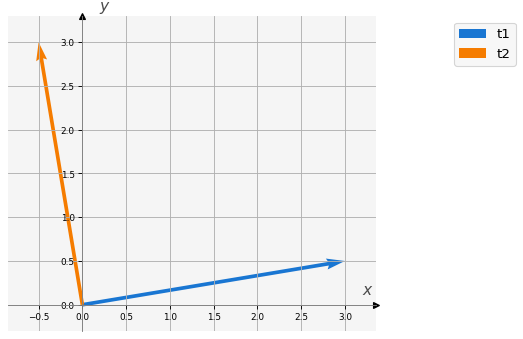
\includegraphics{05_Matrices_Normas_Eigen_files/figure-pdf/cell-23-output-1.png}

Cada par de renglones o de columnas de una matriz ortogonal, son
ortogonales entre sí. Además la longitud de cada columna o renglón es
igual a 1.

\begin{Shaded}
\begin{Highlighting}[]
\CommentTok{\# Definimos una matriz ortogonal}
\NormalTok{C }\OperatorTok{=}\NormalTok{ np.array([[}\DecValTok{1}\OperatorTok{/}\DecValTok{3}\NormalTok{, }\DecValTok{2}\OperatorTok{/}\DecValTok{3}\NormalTok{, }\OperatorTok{{-}}\DecValTok{2}\OperatorTok{/}\DecValTok{3}\NormalTok{],}
\NormalTok{              [}\OperatorTok{{-}}\DecValTok{2}\OperatorTok{/}\DecValTok{3}\NormalTok{, }\DecValTok{2}\OperatorTok{/}\DecValTok{3}\NormalTok{, }\DecValTok{1}\OperatorTok{/}\DecValTok{3}\NormalTok{],}
\NormalTok{              [}\DecValTok{2}\OperatorTok{/}\DecValTok{3}\NormalTok{, }\DecValTok{1}\OperatorTok{/}\DecValTok{3}\NormalTok{, }\DecValTok{2}\OperatorTok{/}\DecValTok{3}\NormalTok{]])}
\end{Highlighting}
\end{Shaded}

\begin{Shaded}
\begin{Highlighting}[]
\CommentTok{\# Verificamos que es ortogonal}
\NormalTok{np.dot(C, C.T)}
\end{Highlighting}
\end{Shaded}

\begin{verbatim}
array([[1., 0., 0.],
       [0., 1., 0.],
       [0., 0., 1.]])
\end{verbatim}

\begin{Shaded}
\begin{Highlighting}[]
\CommentTok{\# Verificamos ortogonalidad entre renglones}
\NormalTok{np.dot(C[}\DecValTok{0}\NormalTok{], C[}\DecValTok{1}\NormalTok{])}
\end{Highlighting}
\end{Shaded}

\begin{verbatim}
0.0
\end{verbatim}

\begin{Shaded}
\begin{Highlighting}[]
\CommentTok{\# Verificamos ortogonalidad entre columnas}
\NormalTok{np.dot(C[:,}\DecValTok{0}\NormalTok{], C[:,}\DecValTok{1}\NormalTok{])}
\end{Highlighting}
\end{Shaded}

\begin{verbatim}
0.0
\end{verbatim}

\begin{Shaded}
\begin{Highlighting}[]
\CommentTok{\# Verificamos la norma de los renglones}
\NormalTok{np.linalg.norm(C[}\DecValTok{2}\NormalTok{])}
\end{Highlighting}
\end{Shaded}

\begin{verbatim}
1.0
\end{verbatim}

\begin{Shaded}
\begin{Highlighting}[]
\CommentTok{\# Verificamos la norma de las columnas}
\NormalTok{np.linalg.norm(C[}\DecValTok{2}\NormalTok{])}
\end{Highlighting}
\end{Shaded}

\begin{verbatim}
1.0
\end{verbatim}

\section{Matriz transpuesta
conjugada}\label{matriz-transpuesta-conjugada}

La matriz \(A^*\) representa a la matriz \(A\) transpuesta y conjugada.
La matriz \(A^* = {\bar{a}_{ji}}\) se llama también la adjunta de \(A\).

\begin{Shaded}
\begin{Highlighting}[]
\CommentTok{\# Creación de una matriz con valores complejos}
\NormalTok{real }\OperatorTok{=}\NormalTok{ np.arange(}\DecValTok{1}\NormalTok{,}\DecValTok{10}\NormalTok{).reshape(}\DecValTok{3}\NormalTok{,}\DecValTok{3}\NormalTok{)}
\NormalTok{imag }\OperatorTok{=}\NormalTok{ np.arange(}\DecValTok{1}\NormalTok{,}\DecValTok{10}\NormalTok{).reshape(}\DecValTok{3}\NormalTok{,}\DecValTok{3}\NormalTok{)}
\NormalTok{C }\OperatorTok{=}\NormalTok{  real }\OperatorTok{+}\NormalTok{ imag }\OperatorTok{*}\OtherTok{1.0j}
\NormalTok{C}
\end{Highlighting}
\end{Shaded}

\begin{verbatim}
array([[1.+1.j, 2.+2.j, 3.+3.j],
       [4.+4.j, 5.+5.j, 6.+6.j],
       [7.+7.j, 8.+8.j, 9.+9.j]])
\end{verbatim}

\begin{Shaded}
\begin{Highlighting}[]
\CommentTok{\# Transpuesta conjugada}
\NormalTok{C.conj().T}
\end{Highlighting}
\end{Shaded}

\begin{verbatim}
array([[1.-1.j, 4.-4.j, 7.-7.j],
       [2.-2.j, 5.-5.j, 8.-8.j],
       [3.-3.j, 6.-6.j, 9.-9.j]])
\end{verbatim}

\section{Matriz definida positiva}\label{matriz-definida-positiva}

Una matriz \(A\) se denomina \textbf{positiva definida} si
\(\langle A\vec{x}, \vec{x}\rangle = \vec{x}^T A\vec{x} > 0\) para
cualquier vector no nulo \(\vec{x}\) de \(\mathbb{R}^n\).

La matriz se llama \textbf{positiva semidefinida} si
\(\vec{x}^T A\vec{x} \ge 0\) para cualquier vector \(\vec{x}\) de
\(\mathbb{R}^n\).

Recordemos que: \[
\vec{x}^T A\vec{x} = \sum_{i=1}^n \sum_{j=1}^n a_{ij} x_i x_j
\]

\section{\texorpdfstring{\textbf{Ejemplo
1.}}{Ejemplo 1.}}\label{ejemplo-1.-2}

Las siguientes dos rectas se cruzan en algún punto.

\[
\begin{array}{ccc}
3x + 2y & = &2 \\
2x + 6y & = &-8
\end{array}
\]

En términos de un sistema lineal, las dos ecuaciones anteriores se
escriben como sigue:

\[
\left[
\begin{array}{cc}
3 & 2 \\
2 & 6
\end{array} \right]
\left[
\begin{array}{c}
x \\
y
\end{array} \right] =
\left[
\begin{array}{c}
2 \\ 
-8
\end{array} \right]
\tag{1}
\]

Podemos calcular \(\vec{x}^T A\vec{x}\) para este ejemplo como sigue:\\

\begin{Shaded}
\begin{Highlighting}[]
\CommentTok{\# Usaremos sympy.}
\CommentTok{\# Primero definimos los símbolos}
\NormalTok{x, y }\OperatorTok{=}\NormalTok{ sympy.symbols(}\StringTok{\textquotesingle{}x y\textquotesingle{}}\NormalTok{)}

\CommentTok{\# Construimos el vector de incógnitas}
\NormalTok{X }\OperatorTok{=}\NormalTok{ sympy.Matrix([x, y])}
\BuiltInTok{print}\NormalTok{(X)}

\CommentTok{\# Construimos la matriz}
\NormalTok{A }\OperatorTok{=}\NormalTok{ sympy.Matrix([[}\FloatTok{3.0}\NormalTok{, }\FloatTok{2.0}\NormalTok{], [}\FloatTok{2.0}\NormalTok{, }\FloatTok{6.0}\NormalTok{]])}
\BuiltInTok{print}\NormalTok{(A)}
\end{Highlighting}
\end{Shaded}

\begin{verbatim}
Matrix([[x], [y]])
Matrix([[3.00000000000000, 2.00000000000000], [2.00000000000000, 6.00000000000000]])
\end{verbatim}

\begin{Shaded}
\begin{Highlighting}[]
\CommentTok{\# Calculamos xT * A * x}
\NormalTok{pos\_def }\OperatorTok{=}\NormalTok{ X.T }\OperatorTok{@}\NormalTok{ A }\OperatorTok{@}\NormalTok{ X}
\NormalTok{pos\_def}
\end{Highlighting}
\end{Shaded}

$\displaystyle \left[\begin{matrix}x \left(3.0 x + 2.0 y\right) + y \left(2.0 x + 6.0 y\right)\end{matrix}\right]$

\begin{Shaded}
\begin{Highlighting}[]
\CommentTok{\# Simplificamos}
\NormalTok{f }\OperatorTok{=}\NormalTok{ sympy.simplify(pos\_def)}
\NormalTok{f}
\end{Highlighting}
\end{Shaded}

$\displaystyle \left[\begin{matrix}3.0 x^{2} + 4.0 x y + 6.0 y^{2}\end{matrix}\right]$

\begin{Shaded}
\begin{Highlighting}[]
\CommentTok{\# Graficamos}
\NormalTok{sympy.plotting.plot3d(f[}\DecValTok{0}\NormalTok{], (x, }\OperatorTok{{-}}\DecValTok{3}\NormalTok{, }\DecValTok{6}\NormalTok{), (y, }\OperatorTok{{-}}\DecValTok{8}\NormalTok{, }\DecValTok{6}\NormalTok{))}
\end{Highlighting}
\end{Shaded}

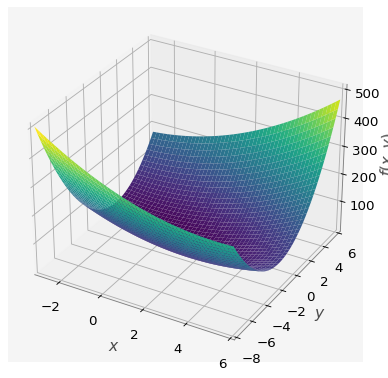
\includegraphics{05_Matrices_Normas_Eigen_files/figure-pdf/cell-35-output-1.png}

Observa que se obtiene una función cuadrática cuya gráfica es un
paraboloide orientado hacia arriba. Esta es una característica de las
matrices definidas positivas.

\section{\texorpdfstring{\textbf{Ejercicio
1.}}{Ejercicio 1.}}\label{ejercicio-1.-4}

Determinar si en el siguiente sistema de ecuaciones se tiene una matriz
definida positiva: \[
\begin{array}{ccc}
y & = & 0.10 x + 200 \\
y & = & 0.30 x + 20
\end{array}
\]

Sistema lineal.

\[
\left[
\begin{array}{cc}
0.10 & -1 \\
0.30 & -1
\end{array} \right]
\left[
\begin{array}{c}
x \\
y
\end{array} \right] =
\left[
\begin{array}{c}
-200 \\ 
-20
\end{array} \right] \tag{2}
\]

Guarda tu respuesta en la variable
\texttt{respuesta\ =\ \textquotesingle{}SI\textquotesingle{}} si la
matriz es definida positiva o
\texttt{respuesta\ =\ \ \textquotesingle{}NO\textquotesingle{}} en caso
contrario.

\textbf{Hint}: Utilizar el mismo código del ejemplo 1 y modificarlo de
acuerdo al ejercicio planteado. Observa cómo sale la gráfica y responde
la pregunta. Para un mejor resultado, utiliza valores muy grandes y muy
chicos en los rangos de \(x\) y \(y\) al momento de graficar (
\textgreater{} 2000).

\begin{Shaded}
\begin{Highlighting}[]
\CommentTok{\# B = sympy.Matrix(...)}
\CommentTok{\# pos\_def\_B = ...}
\CommentTok{\# fB = ...}
\CommentTok{\# sympy.plotting.plot3D( ...)}

\CommentTok{\#\#\# }\RegionMarkerTok{BEGIN}\CommentTok{ SOLUTION}
\NormalTok{B }\OperatorTok{=}\NormalTok{ sympy.Matrix([[}\FloatTok{0.10}\NormalTok{, }\OperatorTok{{-}}\FloatTok{1.0}\NormalTok{], [}\FloatTok{0.30}\NormalTok{, }\OperatorTok{{-}}\FloatTok{1.0}\NormalTok{]])}

\NormalTok{pos\_indef\_B }\OperatorTok{=}\NormalTok{ X.T }\OperatorTok{@}\NormalTok{ B }\OperatorTok{@}\NormalTok{ X}
\NormalTok{fB }\OperatorTok{=}\NormalTok{ sympy.simplify(pos\_indef\_B)}
\NormalTok{sympy.plotting.plot3d(fB[}\DecValTok{0}\NormalTok{], (x, }\OperatorTok{{-}}\DecValTok{6000}\NormalTok{, }\DecValTok{6000}\NormalTok{), (y, }\OperatorTok{{-}}\DecValTok{3000}\NormalTok{, }\DecValTok{3000}\NormalTok{))}
\CommentTok{\#\#\# }\RegionMarkerTok{END}\CommentTok{ SOLUTION}

\CommentTok{\# respuesta = ...}
\end{Highlighting}
\end{Shaded}

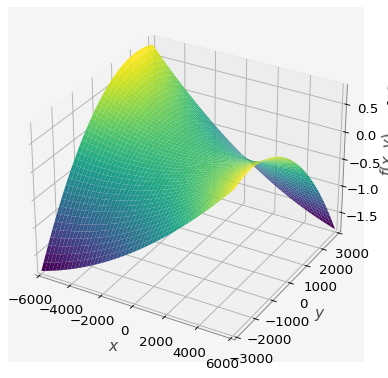
\includegraphics{05_Matrices_Normas_Eigen_files/figure-pdf/cell-36-output-1.png}

\section{Eigenvalores y
Eigenvectores}\label{eigenvalores-y-eigenvectores}

Si \(A\) es una matriz cuadrada, entonces definimos el número
\(\lambda\) (real o complejo) como \textbf{autovalor} (\textbf{valor
propio} o \textbf{eigenvalor}) de \(A\) si
\(A\vec{u} = \lambda \vec{u}\), o equivalentemente si
\(det(A - \lambda I) = 0\). El vector \(\vec{u}\) se llama autovector
(vector propio o eigenvector) de \(A\). El conjunto de todos los
autovalores de la matriz \(A\) se denomina espectro de \(A\) y se denota
como \(\rho(A)\).

\begin{Shaded}
\begin{Highlighting}[]
\CommentTok{\# Convertimos la matriz A a un arreglo de numpy}
\NormalTok{A }\OperatorTok{=}\NormalTok{ np.array(A, dtype}\OperatorTok{=}\BuiltInTok{float}\NormalTok{)}
\NormalTok{A}
\end{Highlighting}
\end{Shaded}

\begin{verbatim}
array([[3., 2.],
       [2., 6.]])
\end{verbatim}

Los eigenvalores y eigenvectores se pueden calcular usando la función
\texttt{np.linalg.eig()\}} \texttt{de\ numpy} como sigue:

\begin{Shaded}
\begin{Highlighting}[]
\NormalTok{np.linalg.eig(A)  }\CommentTok{\# w: eigenvalues, v: eigenvectors}
\end{Highlighting}
\end{Shaded}

\begin{verbatim}
EigResult(eigenvalues=array([2., 7.]), eigenvectors=array([[-0.89442719, -0.4472136 ],
       [ 0.4472136 , -0.89442719]]))
\end{verbatim}

También podemos usar la función \texttt{macti.matem.eigen\_land()} para
obtener mayor información de los eigenvalores y eigenvectores como
sigue:

\begin{Shaded}
\begin{Highlighting}[]
\NormalTok{wA, vA }\OperatorTok{=}\NormalTok{ mmat.eigen\_land(A)}
\end{Highlighting}
\end{Shaded}

\begin{verbatim}
eigenvalores = [2. 7.]
eigenvectores:
 [-0.89442719  0.4472136 ] 
 [-0.4472136  -0.89442719]
ángulo entre eigenvectores = 90.0
\end{verbatim}

Podemos graficar los eigenvectores:

\begin{Shaded}
\begin{Highlighting}[]
\NormalTok{v }\OperatorTok{=}\NormalTok{ mvis.Plotter()}
\NormalTok{v.set\_coordsys()}
\NormalTok{v.plot\_vectors(}\DecValTok{1}\NormalTok{, [vA[:,}\DecValTok{0}\NormalTok{], vA[:,}\DecValTok{1}\NormalTok{]], [}\StringTok{\textquotesingle{}$e\_0\^{}A$\textquotesingle{}}\NormalTok{,}\StringTok{\textquotesingle{}$e\_1\^{}A$\textquotesingle{}}\NormalTok{])}
\NormalTok{v.grid()}
\end{Highlighting}
\end{Shaded}

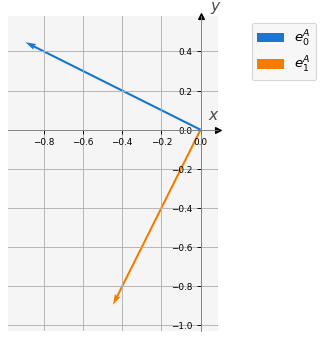
\includegraphics{05_Matrices_Normas_Eigen_files/figure-pdf/cell-40-output-1.png}

Observa que en este caso los eigenvectores son ortogonales.

La relación

\[
A \vec{u} = \lambda \vec{u}
\]

indica básicamente que al aplicar la matriz \(A\) a un eigenvector
\(\vec{u}\), el resultado es el mismo vector escalado
\(\lambda \vec{u}\), es decir no lo rota. Cualquier otro vector, que no
sea un múltiplo de los eigenvectores, será rotado. Veamos esto en el
siguiente código:

\begin{Shaded}
\begin{Highlighting}[]
\CommentTok{\# definimos un vector}
\NormalTok{x1 }\OperatorTok{=}\NormalTok{ np.array([}\FloatTok{0.5}\NormalTok{,}\FloatTok{0.1}\NormalTok{])}

\CommentTok{\# Aplicamos la matriz A}
\NormalTok{r1 }\OperatorTok{=}\NormalTok{ A }\OperatorTok{@}\NormalTok{ x1}

\CommentTok{\# Ahora graficamos}
\NormalTok{v }\OperatorTok{=}\NormalTok{ mvis.Plotter()}
\NormalTok{v.set\_coordsys()}
\NormalTok{v.plot\_vectors(}\DecValTok{1}\NormalTok{, [x1, r1, vA[:,}\DecValTok{0}\NormalTok{], A }\OperatorTok{@}\NormalTok{ vA[:,}\DecValTok{0}\NormalTok{]], }
\NormalTok{                  [}\StringTok{\textquotesingle{}$x\_1$\textquotesingle{}}\NormalTok{, }\StringTok{\textquotesingle{}$A * x\_1$\textquotesingle{}}\NormalTok{, }\StringTok{\textquotesingle{}$e\_0\^{}A$\textquotesingle{}}\NormalTok{, }\StringTok{\textquotesingle{}$A * e\_0\^{}A$\textquotesingle{}}\NormalTok{])}
\NormalTok{v.grid()}
\end{Highlighting}
\end{Shaded}

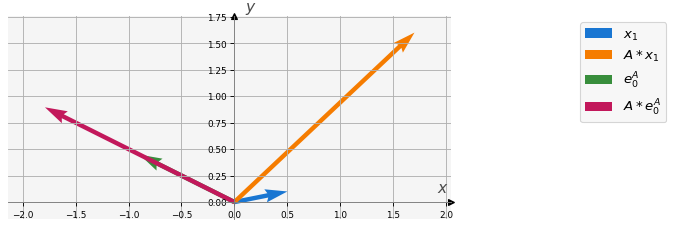
\includegraphics{05_Matrices_Normas_Eigen_files/figure-pdf/cell-41-output-1.png}

Observamos que el eigenvectpr \(e_0^A\) no rota cuando se le aplica
\(A\), pero el vector \(\vec{x}_1\) si es rotado un cierto ángulo cuando
le aplicamos la matriz \(A\).

\section{Normas Matriciales.}\label{normas-matriciales.}

La norma de una matriz \(A\) es un número real positivo denotado por
\(||A||\). Dadas cualesquiera dos matrices \(A\) y \(B\) se cumplen los
siguiente axiomas. 1. \(||A|| \ge 0\). 2. \(||A|| = 0 \iff A = 0\). 3.
\(||aA|| = |a| ||A||\) para cualquier número real \(a\). 4.
\(||A+B|| \le ||A|| + ||B||\) (desigualdad triangular). 5.
\(||AB|| \le ||A||||B||\) (compatibilidad).

Definimos la siguiente matriz

\[
M =
\begin{bmatrix}
-3 & 2 \\
1 & -5
\end{bmatrix}
\]

\begin{Shaded}
\begin{Highlighting}[]
\NormalTok{M }\OperatorTok{=}\NormalTok{ np.array([[}\OperatorTok{{-}}\DecValTok{3}\NormalTok{, }\DecValTok{2}\NormalTok{],[}\DecValTok{1}\NormalTok{, }\OperatorTok{{-}}\DecValTok{5}\NormalTok{]])}
\NormalTok{M}
\end{Highlighting}
\end{Shaded}

\begin{verbatim}
array([[-3,  2],
       [ 1, -5]])
\end{verbatim}

\subsection{Norma 1.}\label{norma-1.}

Consiste en sumar los valores absolutos de los elementos de cada
\textbf{columna} y luego calular la suma máxima: \[
||A||_1 = \max_{1 \le j \le n} \left( \sum_{i=1}^n  |a_{ij}| \right)
\]

\begin{Shaded}
\begin{Highlighting}[]
\NormalTok{np.linalg.norm(M,}\DecValTok{1}\NormalTok{)}
\end{Highlighting}
\end{Shaded}

\begin{verbatim}
7.0
\end{verbatim}

\subsection{\texorpdfstring{Norma
\(\infty\).}{Norma \textbackslash infty.}}\label{norma-infty.}

Consiste en sumar los valores absolutos de los elementos de cada
\textbf{renglón} y luego calular la suma máxima: \[
||A||_\infty = \max_{1 \le i \le n} \left( \sum_{j=1}^n  |a_{ij}| \right)
\]

\begin{Shaded}
\begin{Highlighting}[]
\NormalTok{np.linalg.norm(M, np.infty)}
\end{Highlighting}
\end{Shaded}

\begin{verbatim}
6.0
\end{verbatim}

\subsection{Norma de Frobenius}\label{norma-de-frobenius}

\[
||A||_F = \left( \sum_{i=1}^n \sum_{j=1}^n |a_{ij}|^2 \right)^{1/2}
\]

\begin{Shaded}
\begin{Highlighting}[]
\NormalTok{np.linalg.norm(M, }\StringTok{\textquotesingle{}fro\textquotesingle{}}\NormalTok{)}
\end{Highlighting}
\end{Shaded}

\begin{verbatim}
6.244997998398398
\end{verbatim}

\section{\texorpdfstring{\textbf{Ejemplo
2.}}{Ejemplo 2.}}\label{ejemplo-2.-1}

Verificar que se cumplen los 5 axiomas de las normas matriciales para la
Norma 1 usando la matriz \(M\).

\textbf{Propiedad 1}. \(||M||_1 \geq 0\)

\begin{Shaded}
\begin{Highlighting}[]
\NormalTok{M\_n1 }\OperatorTok{=}\NormalTok{ np.linalg.norm(M,}\DecValTok{1}\NormalTok{ )}
\BuiltInTok{print}\NormalTok{(}\StringTok{\textquotesingle{}M =}\CharTok{\textbackslash{}n}\StringTok{ }\SpecialCharTok{\{\}}\StringTok{\textquotesingle{}}\NormalTok{.}\BuiltInTok{format}\NormalTok{(M))}
\BuiltInTok{print}\NormalTok{(}\StringTok{\textquotesingle{}∥M∥₁ = }\SpecialCharTok{\{\}}\StringTok{\textquotesingle{}}\NormalTok{.}\BuiltInTok{format}\NormalTok{(M\_n1))}
\end{Highlighting}
\end{Shaded}

\begin{verbatim}
M =
 [[-3  2]
 [ 1 -5]]
∥M∥₁ = 7.0
\end{verbatim}

\textbf{Propiedad 2.}

\begin{Shaded}
\begin{Highlighting}[]
\NormalTok{ZERO }\OperatorTok{=}\NormalTok{ np.array([[}\FloatTok{0.0}\NormalTok{, }\FloatTok{0.0}\NormalTok{], [}\FloatTok{0.0}\NormalTok{, }\FloatTok{0.0}\NormalTok{]])}
\NormalTok{ZERO\_n1 }\OperatorTok{=}\NormalTok{ np.linalg.norm(ZERO,}\DecValTok{1}\NormalTok{)}
\BuiltInTok{print}\NormalTok{(}\StringTok{\textquotesingle{}ZERO = }\CharTok{\textbackslash{}n}\SpecialCharTok{\{\}}\StringTok{\textquotesingle{}}\NormalTok{.}\BuiltInTok{format}\NormalTok{(ZERO))}
\BuiltInTok{print}\NormalTok{(}\StringTok{\textquotesingle{}∥ZERO∥₁ = }\SpecialCharTok{\{\}}\StringTok{\textquotesingle{}}\NormalTok{.}\BuiltInTok{format}\NormalTok{(ZERO\_n1))}
\end{Highlighting}
\end{Shaded}

\begin{verbatim}
ZERO = 
[[0. 0.]
 [0. 0.]]
∥ZERO∥₁ = 0.0
\end{verbatim}

\textbf{Propiedad 3.}

\begin{Shaded}
\begin{Highlighting}[]
\NormalTok{a }\OperatorTok{=} \OperatorTok{{-}}\FloatTok{3.5}
\NormalTok{a\_M\_n1 }\OperatorTok{=}\NormalTok{ np.linalg.norm(a }\OperatorTok{*}\NormalTok{ M, }\DecValTok{1}\NormalTok{) }
\BuiltInTok{print}\NormalTok{(}\StringTok{\textquotesingle{}∥M∥₁ = }\SpecialCharTok{\{\}}\StringTok{, }\CharTok{\textbackslash{}t}\StringTok{ a = }\SpecialCharTok{\{\}}\StringTok{\textquotesingle{}}\NormalTok{.}\BuiltInTok{format}\NormalTok{(M\_n1, a))}
\BuiltInTok{print}\NormalTok{(}\StringTok{\textquotesingle{}}\CharTok{\textbackslash{}n}\StringTok{ ∥a * M∥₁ = }\SpecialCharTok{\{\}}\StringTok{ }\CharTok{\textbackslash{}n}\StringTok{ |a| * ∥M∥₁ = }\SpecialCharTok{\{\}}\StringTok{\textquotesingle{}}\NormalTok{.}\BuiltInTok{format}\NormalTok{(a\_M\_n1, np.}\BuiltInTok{abs}\NormalTok{(a) }\OperatorTok{*}\NormalTok{ M\_n1))}
\end{Highlighting}
\end{Shaded}

\begin{verbatim}
∥M∥₁ = 7.0,      a = -3.5

 ∥a * M∥₁ = 24.5 
 |a| * ∥M∥₁ = 24.5
\end{verbatim}

\textbf{Propiedad 4.}

\begin{Shaded}
\begin{Highlighting}[]
\NormalTok{N }\OperatorTok{=}\NormalTok{ np.arange(}\DecValTok{4}\NormalTok{).reshape(}\DecValTok{2}\NormalTok{,}\DecValTok{2}\NormalTok{)}

\NormalTok{M\_p\_N\_n1}\OperatorTok{=}\NormalTok{ np.linalg.norm(M }\OperatorTok{+}\NormalTok{ N, }\DecValTok{1}\NormalTok{)}

\NormalTok{N\_n1 }\OperatorTok{=}\NormalTok{ np.linalg.norm(N, }\DecValTok{1}\NormalTok{)}

\BuiltInTok{print}\NormalTok{(}\StringTok{\textquotesingle{}}\CharTok{\textbackslash{}n}\StringTok{Norma 1:\textquotesingle{}}\NormalTok{)}
\BuiltInTok{print}\NormalTok{(}\StringTok{\textquotesingle{} ∥M + N∥₁ = }\SpecialCharTok{\{\}}\StringTok{\textquotesingle{}}\NormalTok{.}\BuiltInTok{format}\NormalTok{(M\_p\_N\_n1))}
\BuiltInTok{print}\NormalTok{(}\StringTok{\textquotesingle{} ∥M∥₁ + ∥N∥₁ = }\SpecialCharTok{\{\}}\StringTok{\textquotesingle{}}\NormalTok{.}\BuiltInTok{format}\NormalTok{(M\_n1 }\OperatorTok{+}\NormalTok{ N\_n1))}
\BuiltInTok{print}\NormalTok{(}\StringTok{\textquotesingle{} ¿ ∥M + N∥₁ ≤ ∥M∥₁ + ∥N∥₁ ? : }\SpecialCharTok{\{\}}\StringTok{\textquotesingle{}}\NormalTok{.}\BuiltInTok{format}\NormalTok{(M\_p\_N\_n1 }\OperatorTok{\textless{}=}\NormalTok{ M\_n1 }\OperatorTok{+}\NormalTok{ N\_n1))}
\end{Highlighting}
\end{Shaded}

\begin{verbatim}

Norma 1:
 ∥M + N∥₁ = 6.0
 ∥M∥₁ + ∥N∥₁ = 11.0
 ¿ ∥M + N∥₁ ≤ ∥M∥₁ + ∥N∥₁ ? : True
\end{verbatim}

\textbf{Propiedad 5.}

\begin{Shaded}
\begin{Highlighting}[]
\NormalTok{M\_x\_N\_n1}\OperatorTok{=}\NormalTok{ np.linalg.norm(M }\OperatorTok{*}\NormalTok{ N, }\DecValTok{1}\NormalTok{)}

\BuiltInTok{print}\NormalTok{(}\StringTok{\textquotesingle{}}\CharTok{\textbackslash{}n}\StringTok{Norma 1:\textquotesingle{}}\NormalTok{)}
\BuiltInTok{print}\NormalTok{(}\StringTok{\textquotesingle{} ∥M * N∥₁ = }\SpecialCharTok{\{\}}\StringTok{\textquotesingle{}}\NormalTok{.}\BuiltInTok{format}\NormalTok{(M\_x\_N\_n1))}
\BuiltInTok{print}\NormalTok{(}\StringTok{\textquotesingle{} ∥M∥₁ * ∥N∥₁ = }\SpecialCharTok{\{\}}\StringTok{\textquotesingle{}}\NormalTok{.}\BuiltInTok{format}\NormalTok{(M\_n1 }\OperatorTok{*}\NormalTok{ N\_n1))}
\BuiltInTok{print}\NormalTok{(}\StringTok{\textquotesingle{} ¿ ∥M * N∥₁ ≤ ∥M∥₁ * ∥N∥₁ ? : }\SpecialCharTok{\{\}}\StringTok{\textquotesingle{}}\NormalTok{.}\BuiltInTok{format}\NormalTok{(M\_x\_N\_n1 }\OperatorTok{\textless{}=}\NormalTok{ M\_n1 }\OperatorTok{*}\NormalTok{ N\_n1))}
\end{Highlighting}
\end{Shaded}

\begin{verbatim}

Norma 1:
 ∥M * N∥₁ = 17.0
 ∥M∥₁ * ∥N∥₁ = 28.0
 ¿ ∥M * N∥₁ ≤ ∥M∥₁ * ∥N∥₁ ? : True
\end{verbatim}

\section{\texorpdfstring{\textbf{Ejercicio
2.}}{Ejercicio 2.}}\label{ejercicio-2.-3}

Verificar se cumplen los axiomas de las normas para \(||\cdot||_F\)
usando la matriz \(M\).

\textbf{Propiedad 1.}

El resultado debería ser:

\begin{verbatim}
M =
 [[-3  2]
 [ 1 -5]]
∥M∥F = 6.244997998398398
\end{verbatim}

\begin{Shaded}
\begin{Highlighting}[]
\CommentTok{\#\#\# }\RegionMarkerTok{BEGIN}\CommentTok{ SOLUTION}
\NormalTok{M\_nF }\OperatorTok{=}\NormalTok{ np.linalg.norm(M,}\StringTok{\textquotesingle{}fro\textquotesingle{}}\NormalTok{)}
\BuiltInTok{print}\NormalTok{(}\StringTok{\textquotesingle{}M =}\CharTok{\textbackslash{}n}\StringTok{ }\SpecialCharTok{\{\}}\StringTok{\textquotesingle{}}\NormalTok{.}\BuiltInTok{format}\NormalTok{(M))}
\BuiltInTok{print}\NormalTok{(}\StringTok{\textquotesingle{}∥M∥F = }\SpecialCharTok{\{\}}\StringTok{\textquotesingle{}}\NormalTok{.}\BuiltInTok{format}\NormalTok{(M\_nF))}
\CommentTok{\#\#\# }\RegionMarkerTok{END}\CommentTok{ SOLUTION}
\end{Highlighting}
\end{Shaded}

\begin{verbatim}
M =
 [[-3  2]
 [ 1 -5]]
∥M∥F = 6.244997998398398
\end{verbatim}

\textbf{Propiedad 2.}

El resultado debería ser:

\begin{verbatim}
ZERO = 
[[0. 0.]
 [0. 0.]]
∥ZERO∥F = 0.0
\end{verbatim}

\begin{Shaded}
\begin{Highlighting}[]
\CommentTok{\#\#\# }\RegionMarkerTok{BEGIN}\CommentTok{ SOLUTION}
\NormalTok{ZERO\_nF }\OperatorTok{=}\NormalTok{ np.linalg.norm(ZERO,}\StringTok{\textquotesingle{}fro\textquotesingle{}}\NormalTok{)}
\BuiltInTok{print}\NormalTok{(}\StringTok{\textquotesingle{}ZERO = }\CharTok{\textbackslash{}n}\SpecialCharTok{\{\}}\StringTok{\textquotesingle{}}\NormalTok{.}\BuiltInTok{format}\NormalTok{(ZERO))}
\BuiltInTok{print}\NormalTok{(}\StringTok{\textquotesingle{}∥ZERO∥F = }\SpecialCharTok{\{\}}\StringTok{\textquotesingle{}}\NormalTok{.}\BuiltInTok{format}\NormalTok{(ZERO\_nF))}
\CommentTok{\#\#\# }\RegionMarkerTok{END}\CommentTok{ SOLUTION}
\end{Highlighting}
\end{Shaded}

\begin{verbatim}
ZERO = 
[[0. 0.]
 [0. 0.]]
∥ZERO∥F = 0.0
\end{verbatim}

\textbf{Propiedad 3.}

El resultado debería ser:

\begin{verbatim}
∥M∥F = 6.244997998398398,    a = -3.5

 ∥a * M∥F = 21.857492994394395 
 |a| * ∥M∥F = 21.857492994394395
\end{verbatim}

\begin{Shaded}
\begin{Highlighting}[]
\CommentTok{\#\#\# }\RegionMarkerTok{BEGIN}\CommentTok{ SOLUTION}
\NormalTok{a }\OperatorTok{=} \OperatorTok{{-}}\FloatTok{3.5}
\NormalTok{a\_M\_nF }\OperatorTok{=}\NormalTok{ np.linalg.norm(a }\OperatorTok{*}\NormalTok{ M, }\StringTok{\textquotesingle{}fro\textquotesingle{}}\NormalTok{) }
\BuiltInTok{print}\NormalTok{(}\StringTok{\textquotesingle{}∥M∥F = }\SpecialCharTok{\{\}}\StringTok{, }\CharTok{\textbackslash{}t}\StringTok{ a = }\SpecialCharTok{\{\}}\StringTok{\textquotesingle{}}\NormalTok{.}\BuiltInTok{format}\NormalTok{(M\_nF, a))}
\BuiltInTok{print}\NormalTok{(}\StringTok{\textquotesingle{}}\CharTok{\textbackslash{}n}\StringTok{ ∥a * M∥F = }\SpecialCharTok{\{\}}\StringTok{ }\CharTok{\textbackslash{}n}\StringTok{ |a| * ∥M∥F = }\SpecialCharTok{\{\}}\StringTok{\textquotesingle{}}\NormalTok{.}\BuiltInTok{format}\NormalTok{(a\_M\_nF, np.}\BuiltInTok{abs}\NormalTok{(a) }\OperatorTok{*}\NormalTok{ M\_nF))}
\CommentTok{\#\#\# }\RegionMarkerTok{END}\CommentTok{ SOLUTION}
\end{Highlighting}
\end{Shaded}

\begin{verbatim}
∥M∥F = 6.244997998398398,    a = -3.5

 ∥a * M∥F = 21.857492994394395 
 |a| * ∥M∥F = 21.857492994394395
\end{verbatim}

\textbf{Propiedad 4.}

El resultado debería ser:

\begin{verbatim}
Norma de Frobenius:
 ∥M + N∥F = 5.5677643628300215
 ∥M∥F + ∥N∥F = 9.98665538517234
 ¿ ∥M + N∥F ≤ ∥M∥F + ∥N∥F ? : True
\end{verbatim}

\begin{Shaded}
\begin{Highlighting}[]
\CommentTok{\#\#\# }\RegionMarkerTok{BEGIN}\CommentTok{ SOLUTION}
\NormalTok{N }\OperatorTok{=}\NormalTok{ np.arange(}\DecValTok{4}\NormalTok{).reshape(}\DecValTok{2}\NormalTok{,}\DecValTok{2}\NormalTok{)}

\NormalTok{M\_p\_N\_nF}\OperatorTok{=}\NormalTok{ np.linalg.norm(M }\OperatorTok{+}\NormalTok{ N, }\StringTok{\textquotesingle{}fro\textquotesingle{}}\NormalTok{)}

\NormalTok{N\_nF }\OperatorTok{=}\NormalTok{ np.linalg.norm(N, }\StringTok{\textquotesingle{}fro\textquotesingle{}}\NormalTok{)}

\BuiltInTok{print}\NormalTok{(}\StringTok{\textquotesingle{}}\CharTok{\textbackslash{}n}\StringTok{Norma de Frobenius:\textquotesingle{}}\NormalTok{)}
\BuiltInTok{print}\NormalTok{(}\StringTok{\textquotesingle{} ∥M + N∥F = }\SpecialCharTok{\{\}}\StringTok{\textquotesingle{}}\NormalTok{.}\BuiltInTok{format}\NormalTok{(M\_p\_N\_nF))}
\BuiltInTok{print}\NormalTok{(}\StringTok{\textquotesingle{} ∥M∥F + ∥N∥F = }\SpecialCharTok{\{\}}\StringTok{\textquotesingle{}}\NormalTok{.}\BuiltInTok{format}\NormalTok{(M\_nF }\OperatorTok{+}\NormalTok{ N\_nF))}
\BuiltInTok{print}\NormalTok{(}\StringTok{\textquotesingle{} ¿ ∥M + N∥F ≤ ∥M∥F + ∥N∥F ? : }\SpecialCharTok{\{\}}\StringTok{\textquotesingle{}}\NormalTok{.}\BuiltInTok{format}\NormalTok{(M\_p\_N\_nF }\OperatorTok{\textless{}=}\NormalTok{ M\_nF }\OperatorTok{+}\NormalTok{ N\_nF))}
\CommentTok{\#\#\# }\RegionMarkerTok{END}\CommentTok{ SOLUTION}
\end{Highlighting}
\end{Shaded}

\begin{verbatim}

Norma de Frobenius:
 ∥M + N∥F = 5.5677643628300215
 ∥M∥F + ∥N∥F = 9.98665538517234
 ¿ ∥M + N∥F ≤ ∥M∥F + ∥N∥F ? : True
\end{verbatim}

\textbf{Propiedad 5.}

El resultado debería ser:

\begin{verbatim}
Norma de Frobenius:
 ∥M * N∥F = 15.264337522473747
 ∥M∥F * ∥N∥F = 23.366642891095847
 ¿ ∥M * N∥F ≤ ∥M∥F * ∥N∥F ? : True
\end{verbatim}

\begin{Shaded}
\begin{Highlighting}[]
\CommentTok{\#\#\# }\RegionMarkerTok{BEGIN}\CommentTok{ SOLUTION}
\NormalTok{M\_x\_N\_nF}\OperatorTok{=}\NormalTok{ np.linalg.norm(M }\OperatorTok{*}\NormalTok{ N, }\StringTok{\textquotesingle{}fro\textquotesingle{}}\NormalTok{)}

\BuiltInTok{print}\NormalTok{(}\StringTok{\textquotesingle{}}\CharTok{\textbackslash{}n}\StringTok{Norma de Frobenius:\textquotesingle{}}\NormalTok{)}
\BuiltInTok{print}\NormalTok{(}\StringTok{\textquotesingle{} ∥M * N∥F = }\SpecialCharTok{\{\}}\StringTok{\textquotesingle{}}\NormalTok{.}\BuiltInTok{format}\NormalTok{(M\_x\_N\_nF))}
\BuiltInTok{print}\NormalTok{(}\StringTok{\textquotesingle{} ∥M∥F * ∥N∥F = }\SpecialCharTok{\{\}}\StringTok{\textquotesingle{}}\NormalTok{.}\BuiltInTok{format}\NormalTok{(M\_nF }\OperatorTok{*}\NormalTok{ N\_nF))}
\BuiltInTok{print}\NormalTok{(}\StringTok{\textquotesingle{} ¿ ∥M * N∥F ≤ ∥M∥F * ∥N∥F ? : }\SpecialCharTok{\{\}}\StringTok{\textquotesingle{}}\NormalTok{.}\BuiltInTok{format}\NormalTok{(M\_x\_N\_nF }\OperatorTok{\textless{}=}\NormalTok{ M\_nF }\OperatorTok{*}\NormalTok{ N\_nF))}
\CommentTok{\#\#\# }\RegionMarkerTok{END}\CommentTok{ SOLUTION}
\end{Highlighting}
\end{Shaded}

\begin{verbatim}

Norma de Frobenius:
 ∥M * N∥F = 15.264337522473747
 ∥M∥F * ∥N∥F = 23.366642891095847
 ¿ ∥M * N∥F ≤ ∥M∥F * ∥N∥F ? : True
\end{verbatim}

\subsection{Número de condición}\label{nuxfamero-de-condiciuxf3n}

El número de condición de una matriz \(A\) se define como

\[
\kappa(A) = ||A|| \; ||A^{-1}||
\]

Este número siempre es más grande o igual a 1. Además nos da información
acerca de que tan bien o mal está definido un problema que depende de la
matriz en cuestión. Entre más grande sea este número es más difícil de
resolver el problema.

\begin{Shaded}
\begin{Highlighting}[]
\NormalTok{A }\OperatorTok{=}\NormalTok{ np.array([[}\FloatTok{3.}\NormalTok{, }\FloatTok{2.}\NormalTok{],[}\FloatTok{2.}\NormalTok{, }\FloatTok{6.}\NormalTok{]])}
\BuiltInTok{print}\NormalTok{(A)}
\CommentTok{\# Calculamos el número de condición usando funciones de numpy}
\NormalTok{kA\_F }\OperatorTok{=}\NormalTok{ np.linalg.norm(A, }\StringTok{\textquotesingle{}fro\textquotesingle{}}\NormalTok{) }\OperatorTok{*}\NormalTok{ np.linalg.norm(np.linalg.inv(A), }\StringTok{\textquotesingle{}fro\textquotesingle{}}\NormalTok{)}
\BuiltInTok{print}\NormalTok{(}\StringTok{\textquotesingle{}𝜅(A) = }\SpecialCharTok{\{\}}\StringTok{\textquotesingle{}}\NormalTok{.}\BuiltInTok{format}\NormalTok{(kA\_F))}
\end{Highlighting}
\end{Shaded}

\begin{verbatim}
[[3. 2.]
 [2. 6.]]
𝜅(A) = 3.7857142857142847
\end{verbatim}

\begin{Shaded}
\begin{Highlighting}[]
\CommentTok{\# Existe una función para calcular el número de condición directamente}
\NormalTok{kA\_F }\OperatorTok{=}\NormalTok{ np.linalg.cond(A, }\StringTok{\textquotesingle{}fro\textquotesingle{}}\NormalTok{)}
\BuiltInTok{print}\NormalTok{(}\StringTok{\textquotesingle{}𝜅(A) = }\SpecialCharTok{\{\}}\StringTok{\textquotesingle{}}\NormalTok{.}\BuiltInTok{format}\NormalTok{(kA\_F))}
\end{Highlighting}
\end{Shaded}

\begin{verbatim}
𝜅(A) = 3.7857142857142847
\end{verbatim}

\begin{Shaded}
\begin{Highlighting}[]
\CommentTok{\# Matriz con un número de condición más grande}
\NormalTok{B }\OperatorTok{=}\NormalTok{ np.array([[}\FloatTok{0.10}\NormalTok{, }\OperatorTok{{-}}\DecValTok{1}\NormalTok{],[}\FloatTok{0.30}\NormalTok{, }\OperatorTok{{-}}\DecValTok{1}\NormalTok{]])}
\NormalTok{kB\_F }\OperatorTok{=}\NormalTok{ np.linalg.cond(B, }\StringTok{\textquotesingle{}fro\textquotesingle{}}\NormalTok{)}
\BuiltInTok{print}\NormalTok{(B)}
\BuiltInTok{print}\NormalTok{(}\StringTok{\textquotesingle{}𝜅(B) = }\SpecialCharTok{\{\}}\StringTok{\textquotesingle{}}\NormalTok{.}\BuiltInTok{format}\NormalTok{(kB\_F))}
\end{Highlighting}
\end{Shaded}

\begin{verbatim}
[[ 0.1 -1. ]
 [ 0.3 -1. ]]
𝜅(B) = 10.5
\end{verbatim}

\begin{Shaded}
\begin{Highlighting}[]
\CommentTok{\# Matriz mal condicionada}
\NormalTok{C }\OperatorTok{=}\NormalTok{ np.array([[}\FloatTok{0.10}\NormalTok{, }\OperatorTok{{-}}\DecValTok{1000}\NormalTok{],[}\FloatTok{0.30}\NormalTok{, }\OperatorTok{{-}}\DecValTok{1}\NormalTok{]])}
\NormalTok{kC\_F }\OperatorTok{=}\NormalTok{ np.linalg.cond(C, }\StringTok{\textquotesingle{}fro\textquotesingle{}}\NormalTok{)}
\BuiltInTok{print}\NormalTok{(C)}
\BuiltInTok{print}\NormalTok{(}\StringTok{\textquotesingle{}𝜅(C) = }\SpecialCharTok{\{\}}\StringTok{\textquotesingle{}}\NormalTok{.}\BuiltInTok{format}\NormalTok{(kC\_F))}
\end{Highlighting}
\end{Shaded}

\begin{verbatim}
[[ 1.e-01 -1.e+03]
 [ 3.e-01 -1.e+00]]
𝜅(C) = 3334.448482827609
\end{verbatim}

\section{\texorpdfstring{\textbf{Ejercicio
3.}}{Ejercicio 3.}}\label{ejercicio-3.-1}

Calcula el número de condición para las matrices \(A\), \(B\) y \(C\)
usando las normas 1 y 2. Utiliza la función \texttt{print()} de tal
manera que obtengas una salida similar a la siguiente:

\begin{verbatim}
Número de condición con la norma 1:
 𝜅(A) = ...
 𝜅(B) = ...
 𝜅(C) = ...
Número de condición con la norma 2:
 𝜅(A) = ... 
 𝜅(B) = ...
 𝜅(C) = ...
\end{verbatim}

\begin{Shaded}
\begin{Highlighting}[]
\CommentTok{\# Con la norma 1}
\CommentTok{\# kA\_1 = ...}
\CommentTok{\# ...}
\CommentTok{\# print(\textquotesingle{}Número ...)}
\CommentTok{\# print(\textquotesingle{}𝜅(A) = \{\}, ...)}

\CommentTok{\# Con la norma 2}
\CommentTok{\# ...}

\CommentTok{\#\#\# }\RegionMarkerTok{BEGIN}\CommentTok{ SOLUTION}
\CommentTok{\# Usando la norma 1}
\NormalTok{kA\_1 }\OperatorTok{=}\NormalTok{ np.linalg.cond(A, }\DecValTok{1}\NormalTok{)}
\NormalTok{kB\_1 }\OperatorTok{=}\NormalTok{ np.linalg.cond(B, }\DecValTok{1}\NormalTok{)}
\NormalTok{kC\_1 }\OperatorTok{=}\NormalTok{ np.linalg.cond(C, }\DecValTok{1}\NormalTok{)}
\BuiltInTok{print}\NormalTok{(}\StringTok{\textquotesingle{}Número de condición con la norma 1:\textquotesingle{}}\NormalTok{)}
\BuiltInTok{print}\NormalTok{(}\StringTok{\textquotesingle{} 𝜅(A) = }\SpecialCharTok{\{\}}\StringTok{ }\CharTok{\textbackslash{}n}\StringTok{ 𝜅(B) = }\SpecialCharTok{\{\}}\CharTok{\textbackslash{}n}\StringTok{ 𝜅(C) = }\SpecialCharTok{\{\}}\StringTok{\textquotesingle{}}\NormalTok{.}\BuiltInTok{format}\NormalTok{(kA\_1, kB\_1, kC\_1))}

\CommentTok{\# Usando la norma 2}
\NormalTok{kA\_2 }\OperatorTok{=}\NormalTok{ np.linalg.cond(A, }\DecValTok{2}\NormalTok{)}
\NormalTok{kB\_2 }\OperatorTok{=}\NormalTok{ np.linalg.cond(B, }\DecValTok{2}\NormalTok{)}
\NormalTok{kC\_2 }\OperatorTok{=}\NormalTok{ np.linalg.cond(C, }\DecValTok{2}\NormalTok{)}
\BuiltInTok{print}\NormalTok{(}\StringTok{\textquotesingle{}Número de condición con la norma 2:\textquotesingle{}}\NormalTok{)}
\BuiltInTok{print}\NormalTok{(}\StringTok{\textquotesingle{} 𝜅(A) = }\SpecialCharTok{\{\}}\StringTok{ }\CharTok{\textbackslash{}n}\StringTok{ 𝜅(B) = }\SpecialCharTok{\{\}}\CharTok{\textbackslash{}n}\StringTok{ 𝜅(C) = }\SpecialCharTok{\{\}}\StringTok{\textquotesingle{}}\NormalTok{.}\BuiltInTok{format}\NormalTok{(kA\_2, kB\_2, kC\_2))}
\CommentTok{\#\#\# }\RegionMarkerTok{END}\CommentTok{ SOLUTION}
\end{Highlighting}
\end{Shaded}

\begin{verbatim}
Número de condición con la norma 1:
 𝜅(A) = 4.571428571428571 
 𝜅(B) = 13.0
 𝜅(C) = 3338.113037679226
Número de condición con la norma 2:
 𝜅(A) = 3.499999999999999 
 𝜅(B) = 10.40388203202208
 𝜅(C) = 3334.4481829279107
\end{verbatim}

\bookmarksetup{startatroot}

\chapter{Sistemas de ecuaciones lineales:
introducción}\label{sistemas-de-ecuaciones-lineales-introducciuxf3n}

\textbf{Objetivo general} - Plantear y resolver un problema en términos
de la solución de un sistema de ecuaciones lineales.

\textbf{Objetivos particulares} - Entender como plantear un problema en
términos de un sistema de ecuaciones lineales. - Usar funciones de la
biblioteca \texttt{numpy} para resolver el problema. - Comparar varios
métodos para la solución de problemas más complejos.

MACTI NOTES by {Luis Miguel de la Cruz Salas} is licensed under CC
BY-NC-SA 4.0

\textbf{Trabajo realizado con el apoyo del Programa UNAM-DGAPA-PAPIME
PE101922}

\#\# Planes de telefonía móvil.

Dos compañías de telefonía compiten por ganar clientes. En la tabla que
sigue se muestra el costo de la renta y el costo por Megabyte (MB) de
datos de cada compañía.

\begin{longtable}[]{@{}ccc@{}}
\toprule\noalign{}
& Renta mensual & Costo por MB \\
\midrule\noalign{}
\endhead
\bottomrule\noalign{}
\endlastfoot
Compañía A & \(200\) & \(0.10\) \\
Compañía B & \(20\) & \(0.30\) \\
\end{longtable}

\textbf{¿Cómo podríamos decidir cuál de estas companías conviene
contratar?}

\#\#\# Modelo matemático - Observamos en la tabla anterior que la
compañía A tiene un precio fijo de 200 pesos mensuales que es 10 veces
mayor al precio que cobra la compañía B (20 pesos). - Por otro lado, la
compañía B cobra 0.30 pesos por cada MB, que es 3 veces mayor al precio
por MB de la compañía A. - El precio final mensual de cada compañía
depende básicamente de cuantos MB se usen.

Podemos escribir la forma en que cambia el precio de cada compañía en
función de los MB usados:

\$

\begin{array}{ccc}
P_A & = & 0.10 x + 200 \tag{1}\\
P_B & = & 0.30 x + 20
\end{array}

\$

donde \(x\) representa el número de MB usados durante un mes.

\subsection{Ejercicio 1. Gráfica de
rectas.}\label{ejercicio-1.-gruxe1fica-de-rectas.}

En el código siguiente complete las fórmulas para cada compañía de
acuerdo con las ecuaciones dadas en (1) y posteriormente ejecute el
código para obtener una gráfica de cómo cambia el precio en función de
los MB utilizados.

\begin{Shaded}
\begin{Highlighting}[]
\CommentTok{\# Importación de las bibliotecas numpy y matplotlib}
\ImportTok{import}\NormalTok{ numpy }\ImportTok{as}\NormalTok{ np}
\ImportTok{import}\NormalTok{ matplotlib.pyplot }\ImportTok{as}\NormalTok{ plt}
\ImportTok{import}\NormalTok{ sys, macti.visual}

\ImportTok{from}\NormalTok{ macti.evaluation }\ImportTok{import} \OperatorTok{*}
\end{Highlighting}
\end{Shaded}

\begin{Shaded}
\begin{Highlighting}[]
\NormalTok{quizz }\OperatorTok{=}\NormalTok{ Quizz(}\StringTok{\textquotesingle{}06\textquotesingle{}}\NormalTok{, }\StringTok{\textquotesingle{}notebooks\textquotesingle{}}\NormalTok{, }\StringTok{\textquotesingle{}local\textquotesingle{}}\NormalTok{)}
\end{Highlighting}
\end{Shaded}

Fórmulas a implementar: \$

\begin{array}{ccc}
P_A & = & 0.10 x + 200\\
P_B & = & 0.30 x + 20
\end{array}

\$

\begin{Shaded}
\begin{Highlighting}[]
\CommentTok{\# Megabytes desde 0 hasta 1500 (1.5 GB) en pasos de 10.}
\NormalTok{x }\OperatorTok{=}\NormalTok{ np.linspace(}\DecValTok{0}\NormalTok{,}\DecValTok{1500}\NormalTok{,}\DecValTok{10}\NormalTok{)}

\CommentTok{\# Fórmulas de cada compañía}
\CommentTok{\# PA = ...}
\CommentTok{\# PB = ...}
\CommentTok{\#}
\CommentTok{\#\#\# }\RegionMarkerTok{BEGIN}\CommentTok{ SOLUTION}
\NormalTok{PA }\OperatorTok{=} \FloatTok{0.10} \OperatorTok{*}\NormalTok{ x }\OperatorTok{+} \DecValTok{200}
\NormalTok{PB }\OperatorTok{=} \FloatTok{0.30} \OperatorTok{*}\NormalTok{ x }\OperatorTok{+} \DecValTok{20}

\NormalTok{file\_answer }\OperatorTok{=}\NormalTok{ FileAnswer()}
\NormalTok{file\_answer.write(}\StringTok{\textquotesingle{}1\textquotesingle{}}\NormalTok{, PA, }\StringTok{\textquotesingle{}Checa la fórmula para PA\textquotesingle{}}\NormalTok{)}
\NormalTok{file\_answer.write(}\StringTok{\textquotesingle{}2\textquotesingle{}}\NormalTok{, PB, }\StringTok{\textquotesingle{}Checa la fórmula para PB\textquotesingle{}}\NormalTok{)}
\CommentTok{\#\#\# }\RegionMarkerTok{END}\CommentTok{ SOLUTION}

\BuiltInTok{print}\NormalTok{(}\StringTok{\textquotesingle{}PA = }\SpecialCharTok{\{\}}\StringTok{\textquotesingle{}}\NormalTok{.}\BuiltInTok{format}\NormalTok{(PA))}
\BuiltInTok{print}\NormalTok{(}\StringTok{\textquotesingle{}Pb = }\SpecialCharTok{\{\}}\StringTok{\textquotesingle{}}\NormalTok{.}\BuiltInTok{format}\NormalTok{(PB))}
\end{Highlighting}
\end{Shaded}

\begin{verbatim}
El directorio :/home/jovyan/macti_notes/notebooks/.ans/SMM/ ya existe
Respuestas y retroalimentación almacenadas.
PA = [200.         216.66666667 233.33333333 250.         266.66666667
 283.33333333 300.         316.66666667 333.33333333 350.        ]
Pb = [ 20.  70. 120. 170. 220. 270. 320. 370. 420. 470.]
\end{verbatim}

\begin{Shaded}
\begin{Highlighting}[]
\NormalTok{quizz.eval\_numeric(}\StringTok{\textquotesingle{}1\textquotesingle{}}\NormalTok{, PA)}
\end{Highlighting}
\end{Shaded}

\begin{verbatim}
----------------------------------------
1 | Tu resultado es correcto.
----------------------------------------
\end{verbatim}

\begin{Shaded}
\begin{Highlighting}[]
\NormalTok{quizz.eval\_numeric(}\StringTok{\textquotesingle{}2\textquotesingle{}}\NormalTok{, PB)}
\end{Highlighting}
\end{Shaded}

\begin{verbatim}
----------------------------------------
2 | Tu resultado es correcto.
----------------------------------------
\end{verbatim}

\begin{Shaded}
\begin{Highlighting}[]
\CommentTok{\# Gráfica de ambos casos}
\NormalTok{plt.plot(x, PA, label }\OperatorTok{=} \StringTok{\textquotesingle{}Compañía A\textquotesingle{}}\NormalTok{)}
\NormalTok{plt.plot(x, PB, label }\OperatorTok{=} \StringTok{\textquotesingle{}Compañía B\textquotesingle{}}\NormalTok{)}

\CommentTok{\# Decoración de la gráfica}
\NormalTok{plt.xlabel(}\StringTok{\textquotesingle{}MB\textquotesingle{}}\NormalTok{)}
\NormalTok{plt.ylabel(}\StringTok{\textquotesingle{}Precio final\textquotesingle{}}\NormalTok{)}
\NormalTok{plt.legend()}
\NormalTok{plt.grid()}
\NormalTok{plt.show()}
\end{Highlighting}
\end{Shaded}

\includegraphics{06_Sol_Sist_Lineales_Intro_files/figure-pdf/cell-7-output-1.png}

\textbf{¿Qué observamos en la figura anterior?}

Para decidir cuál de los dos compañías elegir, debemos saber cuantos MB
gastamos al mes. En la figura se ve que al principio, con pocos MB
usados conviene contratar a la compañía B. Pero después, si hacemos uso
intenso de nuestras redes sociales, el consumo de MB aumenta y como
consecuencia el precio de la compañía A es más barato.

\textbf{¿Será posible determinar con precisión el punto de cruce de las
rectas?}

\#\#\# Sistema de ecuaciones lineales.

Las ecuaciones \((1)\) tienen la forma típica de una recta:
\(y = m x + b\)

Para la compañía A tenemos que \(m = 0.10\) y \(b = 200\), mientras que
para la compañía B tenemos \(m = 0.35\) y \(b = 20\), entonces
escribimos:

\[
\begin{array}{ccc}
y & = & 0.10 x + 200 \\
y & = & 0.35 x + 20
\end{array}
\]

Ahora, es posible escribir las ecuaciones de las líneas rectas en forma
de un sistema de ecuaciones lineales como sigue:

\[
\left[
\begin{array}{cc}
0.10 & -1 \\
0.35 & -1
\end{array} \right]
\left[
\begin{array}{c}
x \\
y
\end{array} \right] =
\left[
\begin{array}{c}
-200 \\ 
-20
\end{array} \right] \tag{2}
\]

\textbf{¿Puede verificar que el sistema (2) es correcto?}

Si resolvemos el sistema (2) entonces será posible conocer de manera
precisa el cruce de las rectas.

\subsection{Ejercicio 2. Solución del sistema
lineal.}\label{ejercicio-2.-soluciuxf3n-del-sistema-lineal.}

\begin{enumerate}
\def\labelenumi{\arabic{enumi}.}
\tightlist
\item
  En el siguiente código, complete los datos de la matriz \texttt{A} y
  el vector \texttt{b} de acuerdo con el sistema (2).
\end{enumerate}

\begin{Shaded}
\begin{Highlighting}[]
\CommentTok{\# Definimos la matriz A y el vector b}
\CommentTok{\# A = np.array([[],[]])}
\CommentTok{\# B = np.array([[]])}
\CommentTok{\#}
\CommentTok{\#\#\# }\RegionMarkerTok{BEGIN}\CommentTok{ SOLUTION}
\NormalTok{A }\OperatorTok{=}\NormalTok{ np.array([[}\FloatTok{0.10}\NormalTok{, }\OperatorTok{{-}}\FloatTok{1.}\NormalTok{],[}\FloatTok{0.30}\NormalTok{,}\OperatorTok{{-}}\FloatTok{1.}\NormalTok{]] )}
\NormalTok{b }\OperatorTok{=}\NormalTok{ np.array([[}\OperatorTok{{-}}\FloatTok{200.0}\NormalTok{,}\OperatorTok{{-}}\FloatTok{20.0}\NormalTok{]])}

\NormalTok{file\_answer.write(}\StringTok{\textquotesingle{}3\textquotesingle{}}\NormalTok{, A, }\StringTok{\textquotesingle{}Checa los elementos de la matriz A\textquotesingle{}}\NormalTok{)}
\NormalTok{file\_answer.write(}\StringTok{\textquotesingle{}4\textquotesingle{}}\NormalTok{, b, }\StringTok{\textquotesingle{}Checa los elementos del vector b\textquotesingle{}}\NormalTok{)}
\CommentTok{\#\#\# }\RegionMarkerTok{END}\CommentTok{ SOLUTION}

\BuiltInTok{print}\NormalTok{(}\StringTok{"Matriz A : }\CharTok{\textbackslash{}n}\StringTok{"}\NormalTok{,A)}
\BuiltInTok{print}\NormalTok{(}\StringTok{"Vector b : }\CharTok{\textbackslash{}n}\StringTok{"}\NormalTok{, b)}
\end{Highlighting}
\end{Shaded}

\begin{verbatim}
El directorio :/home/jovyan/macti_notes/notebooks/.ans/SMM/ ya existe
Respuestas y retroalimentación almacenadas.
Matriz A : 
 [[ 0.1 -1. ]
 [ 0.3 -1. ]]
Vector b : 
 [[-200.  -20.]]
\end{verbatim}

\begin{Shaded}
\begin{Highlighting}[]
\NormalTok{quizz.eval\_numeric(}\StringTok{\textquotesingle{}3\textquotesingle{}}\NormalTok{, A)}
\end{Highlighting}
\end{Shaded}

\begin{verbatim}
----------------------------------------
3 | Tu resultado es correcto.
----------------------------------------
\end{verbatim}

\begin{Shaded}
\begin{Highlighting}[]
\NormalTok{quizz.eval\_numeric(}\StringTok{\textquotesingle{}4\textquotesingle{}}\NormalTok{, b)}
\end{Highlighting}
\end{Shaded}

\begin{verbatim}
----------------------------------------
4 | Tu resultado es correcto.
----------------------------------------
\end{verbatim}

\begin{enumerate}
\def\labelenumi{\arabic{enumi}.}
\setcounter{enumi}{1}
\tightlist
\item
  Investigue como usar la función numpy.linalg.solve() para resolver el
  sistema de ecuaciones. Resuelva el sistema y guarde la solución en el
  vector \texttt{xsol}.
\end{enumerate}

\begin{Shaded}
\begin{Highlighting}[]
\CommentTok{\# Resolvemos el sistema de ecuaciones lineal}
\CommentTok{\# xsol = np.linalg.solve( ... )}
\CommentTok{\#}
\CommentTok{\#\#\# }\RegionMarkerTok{BEGIN}\CommentTok{ SOLUTION}
\NormalTok{xsol }\OperatorTok{=}\NormalTok{ np.linalg.solve(A,b.T) }

\NormalTok{file\_answer.write(}\StringTok{\textquotesingle{}5\textquotesingle{}}\NormalTok{, xsol, }\StringTok{\textquotesingle{}Verifica que usaste correctamente la función np.linalg.solve()\textquotesingle{}}\NormalTok{)}
\CommentTok{\#\#\# }\RegionMarkerTok{END}\CommentTok{ SOLUTION}

\BuiltInTok{print}\NormalTok{(}\StringTok{"Solución del sistema: }\CharTok{\textbackslash{}n}\StringTok{"}\NormalTok{, xsol)}
\end{Highlighting}
\end{Shaded}

\begin{verbatim}
El directorio :/home/jovyan/macti_notes/notebooks/.ans/SMM/ ya existe
Respuestas y retroalimentación almacenadas.
Solución del sistema: 
 [[900.]
 [290.]]
\end{verbatim}

\begin{Shaded}
\begin{Highlighting}[]
\NormalTok{quizz.eval\_numeric(}\StringTok{\textquotesingle{}5\textquotesingle{}}\NormalTok{, xsol)}
\end{Highlighting}
\end{Shaded}

\begin{verbatim}
----------------------------------------
5 | Tu resultado es correcto.
----------------------------------------
\end{verbatim}

\begin{Shaded}
\begin{Highlighting}[]
\CommentTok{\# Dot product}
\CommentTok{\# rhs = np.dot( ... )}
\CommentTok{\#}
\CommentTok{\#\#\# }\RegionMarkerTok{BEGIN}\CommentTok{ SOLUTION}
\NormalTok{rhs }\OperatorTok{=}\NormalTok{ np.dot(A, xsol)}

\NormalTok{file\_answer.write(}\StringTok{\textquotesingle{}6\textquotesingle{}}\NormalTok{, rhs, }\StringTok{\textquotesingle{}Checa que la representación de cada número sea la correcta.\textquotesingle{}}\NormalTok{)}
\NormalTok{file\_answer.to\_file(}\StringTok{\textquotesingle{}06\textquotesingle{}}\NormalTok{)}
\CommentTok{\#\#\# }\RegionMarkerTok{END}\CommentTok{ SOLUTION}

\BuiltInTok{print}\NormalTok{(rhs)}
\end{Highlighting}
\end{Shaded}

\begin{verbatim}
El directorio :/home/jovyan/macti_notes/notebooks/.ans/SMM/ ya existe
Respuestas y retroalimentación almacenadas.
[[-200.]
 [ -20.]]
\end{verbatim}

\begin{Shaded}
\begin{Highlighting}[]
\NormalTok{quizz.eval\_numeric(}\StringTok{\textquotesingle{}6\textquotesingle{}}\NormalTok{, rhs)}
\end{Highlighting}
\end{Shaded}

\begin{verbatim}
----------------------------------------
6 | Tu resultado es correcto.
----------------------------------------
\end{verbatim}

Si todo se hizo correctamente, el siguiente código debe graficar las
rectas de las dos compañías y en el punto donde se cruzan

\begin{Shaded}
\begin{Highlighting}[]
\CommentTok{\# Gráfica de las líneas de cada compañía}
\NormalTok{plt.plot(x, PA, lw}\OperatorTok{=}\DecValTok{3}\NormalTok{,label }\OperatorTok{=} \StringTok{\textquotesingle{}A\textquotesingle{}}\NormalTok{)}
\NormalTok{plt.plot(x, PB, lw}\OperatorTok{=}\DecValTok{3}\NormalTok{,label }\OperatorTok{=} \StringTok{\textquotesingle{}B\textquotesingle{}}\NormalTok{)}

\CommentTok{\# Punto de cruce de las líneas rectas}
\NormalTok{plt.scatter(xsol[}\DecValTok{0}\NormalTok{], xsol[}\DecValTok{1}\NormalTok{], fc }\OperatorTok{=} \StringTok{\textquotesingle{}C3\textquotesingle{}}\NormalTok{, ec }\OperatorTok{=}\StringTok{\textquotesingle{}k\textquotesingle{}}\NormalTok{, s }\OperatorTok{=} \DecValTok{100}\NormalTok{, alpha}\OperatorTok{=}\FloatTok{0.85}\NormalTok{, zorder}\OperatorTok{=}\DecValTok{5}\NormalTok{, label}\OperatorTok{=}\StringTok{\textquotesingle{}Solución\textquotesingle{}}\NormalTok{)}

\CommentTok{\# Decoración de la gráfica}
\NormalTok{plt.xlabel(}\StringTok{\textquotesingle{}MB\textquotesingle{}}\NormalTok{)}
\NormalTok{plt.ylabel(}\StringTok{\textquotesingle{}Precio final\textquotesingle{}}\NormalTok{)}
\NormalTok{plt.title(}\StringTok{\textquotesingle{}Cruce de las rectas: (}\SpecialCharTok{\{:4.0f\}}\StringTok{ MB, }\SpecialCharTok{\{:4.0f\}}\StringTok{ pesos)\textquotesingle{}}\NormalTok{.}\BuiltInTok{format}\NormalTok{(xsol[}\DecValTok{0}\NormalTok{][}\DecValTok{0}\NormalTok{], xsol[}\DecValTok{1}\NormalTok{][}\DecValTok{0}\NormalTok{]))}
\NormalTok{plt.vlines(xsol[}\DecValTok{0}\NormalTok{][}\DecValTok{0}\NormalTok{], }\DecValTok{0}\NormalTok{, xsol[}\DecValTok{1}\NormalTok{][}\DecValTok{0}\NormalTok{], ls}\OperatorTok{=}\StringTok{\textquotesingle{}{-}{-}\textquotesingle{}}\NormalTok{, lw}\OperatorTok{=}\FloatTok{1.0}\NormalTok{, color}\OperatorTok{=}\StringTok{\textquotesingle{}gray\textquotesingle{}}\NormalTok{)}
\NormalTok{plt.hlines(xsol[}\DecValTok{1}\NormalTok{][}\DecValTok{0}\NormalTok{], }\DecValTok{0}\NormalTok{, xsol[}\DecValTok{0}\NormalTok{][}\DecValTok{0}\NormalTok{], ls}\OperatorTok{=}\StringTok{\textquotesingle{}{-}{-}\textquotesingle{}}\NormalTok{, lw}\OperatorTok{=}\FloatTok{1.0}\NormalTok{, color}\OperatorTok{=}\StringTok{\textquotesingle{}gray\textquotesingle{}}\NormalTok{)}

\NormalTok{plt.grid(}\VariableTok{True}\NormalTok{)}
\NormalTok{plt.legend()}
\NormalTok{plt.show()}
\end{Highlighting}
\end{Shaded}

\includegraphics{06_Sol_Sist_Lineales_Intro_files/figure-pdf/cell-15-output-1.png}

\bookmarksetup{startatroot}

\chapter{Métodos iterativos para la solución de sistemas de ecuaciones
lineales}\label{muxe9todos-iterativos-para-la-soluciuxf3n-de-sistemas-de-ecuaciones-lineales}

\textbf{Objetivo.}

Describir e implementar los algoritmos de Jacobi, Gauss-Seidel y SOR
para la solución de sistemas de ecuaciones lineales.

MACTI-Algebra\_Lineal\_01 by Luis M. de la Cruz is licensed under
Attribution-ShareAlike 4.0 International

Trabajo realizado con el apoyo del Programa UNAM-DGAPA-PAPIME PE101922

\begin{Shaded}
\begin{Highlighting}[]
\ImportTok{import}\NormalTok{ numpy }\ImportTok{as}\NormalTok{ np}
\ImportTok{import}\NormalTok{ ipywidgets }\ImportTok{as}\NormalTok{ widgets}
\ImportTok{import}\NormalTok{ macti.visual }\ImportTok{as}\NormalTok{ mvis}
\end{Highlighting}
\end{Shaded}

\bookmarksetup{startatroot}

\chapter{Cruce de dos rectas.}\label{cruce-de-dos-rectas.}

Las siguientes dos rectas se cruzan en algún punto.

\[
\begin{array}{ccc}
3x + 2y & = &2 \\
2x + 6y & = &-8
\end{array}
\]

Las ecuaciones de las rectas se pueden escribir como:

\[
\begin{array}{ccc}
\dfrac{3}{2}x + y & = & 1 \\
\dfrac{2}{6}x + y & = & -\dfrac{8}{6}
\end{array} \Longrightarrow
\begin{array}{ccc}
y = m_1 x + b_1 \\
y = m_2 x + b_2
\end{array} \text{ donde }
\begin{array}{ccc}
m_1 = -\dfrac{3}{2} & b_1 = 1 \\
m_2 = -\dfrac{2}{6} & b_2 = -\dfrac{8}{6}
\end{array}
\]

Ahora realizaremos la gráfica de las rectas:

\section{Definición y gráfica de las
rectas}\label{definiciuxf3n-y-gruxe1fica-de-las-rectas}

\section{\texorpdfstring{\textbf{Ejercicio
1.}}{Ejercicio 1.}}\label{ejercicio-1.-5}

En la siguiente celda se define el domino \(x\) para las líneas rectas,
los parámetros para construir la línea recta 1 y su construcción. De la
misma manera define los parámetros y construye la recta 2. Si todo lo
hiciste correctamente, la celda de graficación mostrará las gráficas de
las líneas rectas.

\begin{Shaded}
\begin{Highlighting}[]
\ImportTok{from}\NormalTok{ macti.evaluation }\ImportTok{import}\NormalTok{ FileAnswer, Quizz}
\CommentTok{\#file\_anser = FileAnswer()}
\CommentTok{\#quizz = Quizz()}
\end{Highlighting}
\end{Shaded}

\begin{Shaded}
\begin{Highlighting}[]
\CommentTok{\# Dominio}
\NormalTok{x }\OperatorTok{=}\NormalTok{ np.linspace(}\OperatorTok{{-}}\DecValTok{3}\NormalTok{,}\DecValTok{6}\NormalTok{,}\DecValTok{10}\NormalTok{)}

\CommentTok{\# Línea recta 1}
\NormalTok{m1 }\OperatorTok{=} \OperatorTok{{-}}\DecValTok{3}\OperatorTok{/}\DecValTok{2}
\NormalTok{b1 }\OperatorTok{=} \DecValTok{1}
\NormalTok{y1 }\OperatorTok{=}\NormalTok{ m1 }\OperatorTok{*}\NormalTok{ x }\OperatorTok{+}\NormalTok{ b1}

\CommentTok{\# Línea recta 2}
\CommentTok{\# m2 = ...}
\CommentTok{\# b2 = ...}
\CommentTok{\# y2 = ...}

\CommentTok{\#\#\# }\RegionMarkerTok{BEGIN}\CommentTok{ SOLUTION}
\NormalTok{m2 }\OperatorTok{=} \OperatorTok{{-}}\DecValTok{2}\OperatorTok{/}\DecValTok{6}
\NormalTok{b2 }\OperatorTok{=} \OperatorTok{{-}}\DecValTok{8}\OperatorTok{/}\DecValTok{6}
\NormalTok{y2 }\OperatorTok{=}\NormalTok{ m2 }\OperatorTok{*}\NormalTok{ x }\OperatorTok{+}\NormalTok{ b2}

\CommentTok{\#file\_answer(\textquotesingle{}1\textquotesingle{}, m2, \textquotesingle{}m2 incorrecta revisa el valor del parámetro.\textquotesingle{})}
\CommentTok{\#file\_answer(\textquotesingle{}2\textquotesingle{}, b2, \textquotesingle{}b2 incorrecta revisa el valor del parámetro.\textquotesingle{})}
\CommentTok{\#file\_answer(\textquotesingle{}3\textquotesingle{}, y2, \textquotesingle{}y2 no está definida correctamente.\textquotesingle{})}
\CommentTok{\#\#\# }\RegionMarkerTok{END}\CommentTok{ SOLUTION}
\end{Highlighting}
\end{Shaded}

\begin{Shaded}
\begin{Highlighting}[]
\CommentTok{\#quizz.eval\_numeric(\textquotesingle{}1\textquotesingle{}, m2)}
\CommentTok{\#quizz.eval\_numeric(\textquotesingle{}2\textquotesingle{}, b2)}
\CommentTok{\#quizz.eval\_numeric(\textquotesingle{}3\textquotesingle{}, y2)}
\end{Highlighting}
\end{Shaded}

\textbf{Gráfica de las líneas rectas.}

\begin{Shaded}
\begin{Highlighting}[]
\NormalTok{v }\OperatorTok{=}\NormalTok{ mvis.Plotter(}\DecValTok{1}\NormalTok{,}\DecValTok{1}\NormalTok{,[}\BuiltInTok{dict}\NormalTok{(aspect}\OperatorTok{=}\StringTok{\textquotesingle{}equal\textquotesingle{}}\NormalTok{)],title}\OperatorTok{=}\StringTok{\textquotesingle{}Cruce de rectas\textquotesingle{}}\NormalTok{) }
\NormalTok{v.set\_coordsys(}\DecValTok{1}\NormalTok{)}
\NormalTok{v.plot(}\DecValTok{1}\NormalTok{, x, y1, lw }\OperatorTok{=} \DecValTok{3}\NormalTok{, c }\OperatorTok{=} \StringTok{\textquotesingle{}seagreen\textquotesingle{}}\NormalTok{, label }\OperatorTok{=} \StringTok{\textquotesingle{}$3x+2y=2$\textquotesingle{}}\NormalTok{) }\CommentTok{\# Línea recta 1}
\NormalTok{v.plot(}\DecValTok{1}\NormalTok{, x, y2, lw }\OperatorTok{=} \DecValTok{3}\NormalTok{, c }\OperatorTok{=} \StringTok{\textquotesingle{}mediumorchid\textquotesingle{}}\NormalTok{,label }\OperatorTok{=} \StringTok{\textquotesingle{}$2x+6y={-}8$\textquotesingle{}}\NormalTok{) }\CommentTok{\# Línea recta 2}
\NormalTok{v.legend(ncol }\OperatorTok{=} \DecValTok{1}\NormalTok{, frameon}\OperatorTok{=}\VariableTok{True}\NormalTok{, loc}\OperatorTok{=}\StringTok{\textquotesingle{}best\textquotesingle{}}\NormalTok{, bbox\_to\_anchor}\OperatorTok{=}\NormalTok{(}\FloatTok{1.75}\NormalTok{, }\FloatTok{1.05}\NormalTok{))}
\NormalTok{v.grid()}
\NormalTok{v.show()}
\end{Highlighting}
\end{Shaded}

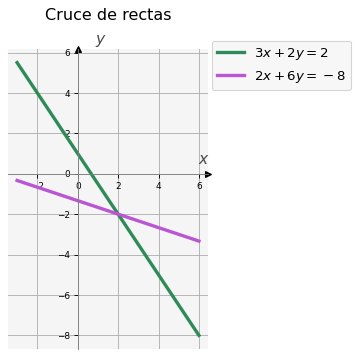
\includegraphics{07_Sol_Sis_Lin_Iter_1_files/figure-pdf/cell-6-output-1.png}

\section{Sistemas lineales.}\label{sistemas-lineales.}

Las ecuaciones de las rectas se pueden escribir en forma de un sistema
lineal:

\[
\left[
\begin{array}{cc}
3 & 2 \\
2 & 6
\end{array} \right]
\left[
\begin{array}{c}
x_{0} \\
x_{1}
\end{array} \right] =
\left[
\begin{array}{c}
2 \\ 
-8
\end{array} \right]
\tag{1}
\]

Podemos calcular el cruce de las rectas resolviendo el sistema lineal:

\section{\texorpdfstring{\textbf{Ejemplo
1.}}{Ejemplo 1.}}\label{ejemplo-1.-3}

Definir el sistema lineal y resolverlo. Posteriomente graficar las
rectas y el punto solución.

El sistema lineal se puede resolver directamente con la función
\texttt{np.linalg.solve()} como sigue:

\begin{Shaded}
\begin{Highlighting}[]
\NormalTok{A }\OperatorTok{=}\NormalTok{ np.array([[}\DecValTok{3}\NormalTok{, }\DecValTok{2}\NormalTok{],[}\DecValTok{2}\NormalTok{,}\DecValTok{6}\NormalTok{]] )}
\NormalTok{b }\OperatorTok{=}\NormalTok{ np.array([[}\DecValTok{2}\NormalTok{,}\OperatorTok{{-}}\DecValTok{8}\NormalTok{]])}
\BuiltInTok{print}\NormalTok{(}\StringTok{"Matriz A : }\CharTok{\textbackslash{}n}\StringTok{"}\NormalTok{,A)}
\BuiltInTok{print}\NormalTok{(}\StringTok{"Vector b : }\CharTok{\textbackslash{}n}\StringTok{"}\NormalTok{, b)}

\NormalTok{sol }\OperatorTok{=}\NormalTok{ np.linalg.solve(A,b[}\DecValTok{0}\NormalTok{]) }\CommentTok{\# Función del módulo linalg para resolver el sistema}
\BuiltInTok{print}\NormalTok{(}\StringTok{"Solución del sistema: "}\NormalTok{, sol)}
\end{Highlighting}
\end{Shaded}

\begin{verbatim}
Matriz A : 
 [[3 2]
 [2 6]]
Vector b : 
 [[ 2 -8]]
Solución del sistema:  [ 2. -2.]
\end{verbatim}

\textbf{Gráfica de las líneas rectas y el punto de cruce (solución).}

\begin{Shaded}
\begin{Highlighting}[]
\NormalTok{v }\OperatorTok{=}\NormalTok{ mvis.Plotter(}\DecValTok{1}\NormalTok{,}\DecValTok{1}\NormalTok{,[}\BuiltInTok{dict}\NormalTok{(aspect}\OperatorTok{=}\StringTok{\textquotesingle{}equal\textquotesingle{}}\NormalTok{)],title}\OperatorTok{=}\StringTok{\textquotesingle{}Cruce de rectas\textquotesingle{}}\NormalTok{) }
\NormalTok{v.set\_coordsys(}\DecValTok{1}\NormalTok{)}
\NormalTok{v.plot(}\DecValTok{1}\NormalTok{, x, y1, lw }\OperatorTok{=} \DecValTok{3}\NormalTok{, c }\OperatorTok{=} \StringTok{\textquotesingle{}seagreen\textquotesingle{}}\NormalTok{, label }\OperatorTok{=} \StringTok{\textquotesingle{}$3x+2y=2$\textquotesingle{}}\NormalTok{) }\CommentTok{\# Línea recta 1}
\NormalTok{v.plot(}\DecValTok{1}\NormalTok{, x, y2, lw }\OperatorTok{=} \DecValTok{3}\NormalTok{, c }\OperatorTok{=} \StringTok{\textquotesingle{}mediumorchid\textquotesingle{}}\NormalTok{, label }\OperatorTok{=} \StringTok{\textquotesingle{}$2x+6y={-}8$\textquotesingle{}}\NormalTok{) }\CommentTok{\# Línea recta 2}
\NormalTok{v.scatter(}\DecValTok{1}\NormalTok{, sol[}\DecValTok{0}\NormalTok{], sol[}\DecValTok{1}\NormalTok{], fc}\OperatorTok{=}\StringTok{\textquotesingle{}sandybrown\textquotesingle{}}\NormalTok{, ec}\OperatorTok{=}\StringTok{\textquotesingle{}k\textquotesingle{}}\NormalTok{, s }\OperatorTok{=} \DecValTok{75}\NormalTok{, alpha}\OperatorTok{=}\FloatTok{0.75}\NormalTok{, zorder}\OperatorTok{=}\DecValTok{5}\NormalTok{, label}\OperatorTok{=}\StringTok{\textquotesingle{}Sol. final\textquotesingle{}}\NormalTok{) }\CommentTok{\# Solución}
\NormalTok{v.legend(ncol }\OperatorTok{=} \DecValTok{1}\NormalTok{, frameon}\OperatorTok{=}\VariableTok{True}\NormalTok{, loc}\OperatorTok{=}\StringTok{\textquotesingle{}best\textquotesingle{}}\NormalTok{, bbox\_to\_anchor}\OperatorTok{=}\NormalTok{(}\FloatTok{1.75}\NormalTok{, }\FloatTok{1.05}\NormalTok{))}
\NormalTok{v.grid()}
\NormalTok{v.show()}
\end{Highlighting}
\end{Shaded}

\includegraphics{07_Sol_Sis_Lin_Iter_1_files/figure-pdf/cell-8-output-1.png}

En general, un sistema de ecuaciones lineales de \(n \times n\) se
escribe como sigue:

\[
\begin{array}{ccccccc}
a_{11}x_1 & + & a_{12}x_2 & +  \dots  + & a_{1n}x_n & = & b_1 \\
a_{21}x_1 & + & a_{22}x_2 & +  \dots + & a_{2n}x_n & = & b_2 \\
\vdots & & \vdots &  & \vdots & & \vdots \\
a_{i1}x_1 & + & a_{i2}x_2 & +  \dots + & a_{in}x_n & = & b_i \\
\vdots & & \vdots &  & \vdots & & \vdots \\
a_{n1}x_1 & + & a_{n2}x_2 & + \dots + & a_{nn}x_n & = & b_n
\end{array}
\]

Es posible usar diferentes métodos para resolver este tipo de sistemas.
Veamos tres de ellos.

\bookmarksetup{startatroot}

\chapter{Método de Jacobi}\label{muxe9todo-de-jacobi}

\begin{itemize}
\item
  En este método, de la primera ecuación se despeja \(x_1\); de la
  segunda ecuación se despeja \(x_2\); y a sí sucesivamente, de tal
  manera que obtenemos: \[
  \begin{eqnarray*}
    x_1 & = &\left( b_1 - (a_{12}x_2 +  \dots  + a_{1n}x_n) \right) / a_{11}  \\
    x_2 & = &\left( b_2 - (a_{21}x_1 +  \dots  + a_{2n}x_n) \right) / a_{22} \\
    \vdots & & \vdots \\
    x_i & = &\left( b_i - (a_{i1}x_1 +  \dots  + a_{in}x_n) \right) / a_{ii} \\
    \vdots & & \vdots \\
    x_n & = &\left( b_n - (a_{n1}x_1 +  \dots  + a_{nn-1}x_{n-1}) \right) / a_{nn}
  \end{eqnarray*}
  \]
\item
  Suponemos ahora que tenemos una solución inicial aproximada
  \(\mathbf{x}^0 = [x_1^0, \dots, x_n^0]\). Usando esta solución
  inicial, es posible hacer una nueva aproximación para obtener
  \(\mathbf{x}^1 = [x_1^1, \dots, x_n^1]\) como sigue:
\end{itemize}

\[
\begin{eqnarray*}
    x_1^1 & = &\left( b_1 - (a_{12}x_2^0 +  \dots  + a_{1n}x_n^0) \right) / a_{11}  \\
    x_2^1 & = &\left( b_2 - (a_{21}x_1^0 +  \dots  + a_{2n}x_n^0) \right) / a_{22} \\
    \vdots & & \vdots \\
    x_i^1 & = &\left( b_i - (a_{i1}x_1^0 +  \dots  + a_{in}x_n^0) \right) / a_{ii} \\
    \vdots & & \vdots \\
    x_n^1 & = &\left( b_n - (a_{n1}x_1^0 +  \dots  + a_{nn-1}x_{n-1}^0) \right) / a_{nn}
\end{eqnarray*}
\]

\begin{itemize}
\tightlist
\item
  En general para \(i = 1, \dots, n\) y \(k = 1, 2, \dots\) tenemos:
\end{itemize}

\[
x_i^k = \frac{1}{a_{i,i}} \left(b_i -  \sum_{j \neq i} a_{i,j} x_j^{k-1} \right)
\]

\begin{itemize}
\tightlist
\item
  En términos de matrices, la \textbf{iteración de Jacobi} se escribe:
  \[
  \mathbf{x}^k = -\mathbf{D}^{-1} \mathbf{B}\mathbf{x}^{k-1} + \mathbf{D}^{-1} \mathbf{b}
  \]
\end{itemize}

donde \(\mathbf{D}\) es la matriz diagonal y
\(\mathbf{B} = \mathbf{A} - \mathbf{D}\).

\begin{itemize}
\tightlist
\item
  El cálculo de cada componente \(x_i^k\) es independiente de las otras
  componentes, por lo que este método se conoce también como de
  \emph{desplazamientos simultáneos}.
\end{itemize}

\section{Algoritmo Jacobi.}\label{algoritmo-jacobi.}

En general, podemos definir el siguiente algoritmo para el método de
Jacobi.

Observa que en este algoritmo hay un ciclo \texttt{while} el cual
termina cuando el error es menor o igual que una tolerancia \texttt{tol}
o se ha alcanzado un número máximo de iteraciones \texttt{kmax}. En la
línea \textbf{11} se calcula el error, que en términos matemáticos se
define como \(error = || \mathbf{x}^k - \mathbf{x}||\) donde
\(\mathbf{x}^k\) es la aproximación de la iteración \(k\)-ésima y
\(\mathbf{x}\) es la solución exacta. En muchas ocasiones no se tiene
acceso a la solución exacta por lo que se compara con la solución de la
iteración anterior, es decir
\(error = || \mathbf{x}^k - \mathbf{x}^{k-1}||\). En los ejemplos que
siguen si tenemos la solución exacta, por lo que haremos la comparación
con ella.

\section{Implementación.}\label{implementaciuxf3n.-1}

\begin{Shaded}
\begin{Highlighting}[]
\KeywordTok{def}\NormalTok{ jacobi(A,b,tol,kmax,xi, yi):}
\NormalTok{    N }\OperatorTok{=} \BuiltInTok{len}\NormalTok{(b[}\DecValTok{0}\NormalTok{])}
\NormalTok{    xnew }\OperatorTok{=}\NormalTok{ np.zeros(N)}
\NormalTok{    xold }\OperatorTok{=}\NormalTok{ np.zeros(N)}
\NormalTok{    x }\OperatorTok{=}\NormalTok{ np.array([}\DecValTok{2}\NormalTok{, }\OperatorTok{{-}}\DecValTok{2}\NormalTok{]) }\CommentTok{\# Solución exacta}
    
    \CommentTok{\# Solución inicial}
\NormalTok{    xold[}\DecValTok{0}\NormalTok{] }\OperatorTok{=}\NormalTok{ xi}
\NormalTok{    xold[}\DecValTok{1}\NormalTok{] }\OperatorTok{=}\NormalTok{ yi}
    
\NormalTok{    xs }\OperatorTok{=}\NormalTok{ [xi]}
\NormalTok{    ys }\OperatorTok{=}\NormalTok{ [yi]}
    
\NormalTok{    e }\OperatorTok{=} \DecValTok{10}
\NormalTok{    error }\OperatorTok{=}\NormalTok{ [] }
    
\NormalTok{    k }\OperatorTok{=} \DecValTok{0}
    \BuiltInTok{print}\NormalTok{(}\StringTok{\textquotesingle{}}\SpecialCharTok{\{:\^{}2\}}\StringTok{ }\SpecialCharTok{\{:\^{}10\}}\StringTok{ }\SpecialCharTok{\{:\^{}12\}}\StringTok{ }\SpecialCharTok{\{:\^{}12\}}\StringTok{\textquotesingle{}}\NormalTok{.}\BuiltInTok{format}\NormalTok{(}\StringTok{\textquotesingle{} i \textquotesingle{}}\NormalTok{, }\StringTok{\textquotesingle{}Error\textquotesingle{}}\NormalTok{, }\StringTok{\textquotesingle{}x0\textquotesingle{}}\NormalTok{, }\StringTok{\textquotesingle{}x1\textquotesingle{}}\NormalTok{))}
    \ControlFlowTok{while}\NormalTok{(e }\OperatorTok{\textgreater{}}\NormalTok{ tol }\KeywordTok{and}\NormalTok{ k }\OperatorTok{\textless{}}\NormalTok{ kmax) :}
        \ControlFlowTok{for}\NormalTok{ i }\KeywordTok{in} \BuiltInTok{range}\NormalTok{(}\DecValTok{0}\NormalTok{,N): }\CommentTok{\# se puede hacer en paralelo}
\NormalTok{            xnew[i] }\OperatorTok{=} \DecValTok{0}
            \ControlFlowTok{for}\NormalTok{ j }\KeywordTok{in} \BuiltInTok{range}\NormalTok{(}\DecValTok{0}\NormalTok{,i):}
\NormalTok{                xnew[i] }\OperatorTok{+=}\NormalTok{ A[i,j] }\OperatorTok{*}\NormalTok{ xold[j]}
            \ControlFlowTok{for}\NormalTok{ j }\KeywordTok{in} \BuiltInTok{range}\NormalTok{(i}\OperatorTok{+}\DecValTok{1}\NormalTok{,N):}
\NormalTok{                xnew[i] }\OperatorTok{+=}\NormalTok{ A[i,j] }\OperatorTok{*}\NormalTok{ xold[j]                }
\NormalTok{            xnew[i] }\OperatorTok{=}\NormalTok{ (b[}\DecValTok{0}\NormalTok{,i] }\OperatorTok{{-}}\NormalTok{ xnew[i]) }\OperatorTok{/}\NormalTok{ A[i,i]}
        
        \CommentTok{\# Almacenamos la solución actual}
\NormalTok{        xs.append(xnew[}\DecValTok{0}\NormalTok{])}
\NormalTok{        ys.append(xnew[}\DecValTok{1}\NormalTok{])}
        
\NormalTok{        e }\OperatorTok{=}\NormalTok{ np.linalg.norm(xnew}\OperatorTok{{-}}\NormalTok{x, }\DecValTok{2}\NormalTok{) }\CommentTok{\# Cálculo del error}
\NormalTok{        error.append(e)}
\NormalTok{        k }\OperatorTok{+=} \DecValTok{1}
\NormalTok{        xold[:] }\OperatorTok{=}\NormalTok{ xnew[:]}
        \BuiltInTok{print}\NormalTok{(}\StringTok{\textquotesingle{}}\SpecialCharTok{\{:2d\}}\StringTok{ }\SpecialCharTok{\{:10.9f\}}\StringTok{ (}\SpecialCharTok{\{:10.9f\}}\StringTok{, }\SpecialCharTok{\{:10.9f\}}\StringTok{)\textquotesingle{}}\NormalTok{.}\BuiltInTok{format}\NormalTok{(k, e, xnew[}\DecValTok{0}\NormalTok{], xnew[}\DecValTok{1}\NormalTok{]))}
    \ControlFlowTok{return}\NormalTok{ xnew, np.array(xs), np.array(ys), error, k}
\end{Highlighting}
\end{Shaded}

\section{\texorpdfstring{\textbf{Ejemplo 3. Aplicación del método de
Jacobi.}}{Ejemplo 3. Aplicación del método de Jacobi.}}\label{ejemplo-3.-aplicaciuxf3n-del-muxe9todo-de-jacobi.}

Haciendo uso de la función \texttt{jacobi} definida en la celda
anterior, aproxima la solución del sistema de ecuaciones (1). Utiliza la
solución inicial \texttt{(xi,\ yi)} = \((-2, 2)\), una tolerancia
\texttt{tol} = \(1 \times 10^{-5}\) y \texttt{kmax} = \(50\)
iteraciones.

\begin{Shaded}
\begin{Highlighting}[]
\CommentTok{\# Solución inicial}
\NormalTok{(xi, yi) }\OperatorTok{=}\NormalTok{ (}\OperatorTok{{-}}\DecValTok{2}\NormalTok{, }\DecValTok{2}\NormalTok{)}
\NormalTok{tol }\OperatorTok{=} \FloatTok{1e{-}5}
\NormalTok{kmax }\OperatorTok{=} \DecValTok{50}

\CommentTok{\# Ejecución del método de Jacobi}
\NormalTok{solJ, xs, ys, eJ, itJ }\OperatorTok{=}\NormalTok{ jacobi(A, b, tol, kmax, xi, yi)}
\end{Highlighting}
\end{Shaded}

\begin{verbatim}
 i    Error         x0           x1     
 1 2.981423970 (-0.666666667, -0.666666667)
 2 1.257078722 (1.111111111, -1.111111111)
 3 0.662538660 (1.407407407, -1.703703704)
 4 0.279350827 (1.802469136, -1.802469136)
 5 0.147230813 (1.868312757, -1.934156379)
 6 0.062077962 (1.956104252, -1.956104252)
 7 0.032717959 (1.970736168, -1.985368084)
 8 0.013795103 (1.990245389, -1.990245389)
 9 0.007270657 (1.993496926, -1.996748463)
10 0.003065578 (1.997832309, -1.997832309)
11 0.001615702 (1.998554873, -1.999277436)
12 0.000681240 (1.999518291, -1.999518291)
13 0.000359045 (1.999678861, -1.999839430)
14 0.000151387 (1.999892954, -1.999892954)
15 0.000079788 (1.999928636, -1.999964318)
16 0.000033641 (1.999976212, -1.999976212)
17 0.000017731 (1.999984141, -1.999992071)
18 0.000007476 (1.999994714, -1.999994714)
\end{verbatim}

Observa que la función \texttt{jacobi()} regresa 5 valores: *
\texttt{solJ} la solución obtenida, * \texttt{xs} y \texttt{ys}
componentes de las soluciones aproximadas en cada paso, * \texttt{eJ} el
error con respecto a la solución exacta e * \texttt{itJ} el número de
iteraciones realizadas.

A continuación graficamos como es que la solución se va aproximando con
este método.

\begin{Shaded}
\begin{Highlighting}[]
\NormalTok{v }\OperatorTok{=}\NormalTok{ mvis.Plotter(}\DecValTok{1}\NormalTok{,}\DecValTok{1}\NormalTok{,[}\BuiltInTok{dict}\NormalTok{(aspect}\OperatorTok{=}\StringTok{\textquotesingle{}equal\textquotesingle{}}\NormalTok{)],title}\OperatorTok{=}\StringTok{\textquotesingle{}Cruce de rectas\textquotesingle{}}\NormalTok{) }
\NormalTok{v.set\_coordsys(}\DecValTok{1}\NormalTok{)}
\NormalTok{v.plot(}\DecValTok{1}\NormalTok{, x, y1, lw }\OperatorTok{=} \DecValTok{3}\NormalTok{, c }\OperatorTok{=} \StringTok{\textquotesingle{}seagreen\textquotesingle{}}\NormalTok{, label }\OperatorTok{=} \StringTok{\textquotesingle{}$3x+2y=2$\textquotesingle{}}\NormalTok{) }\CommentTok{\# Línea recta 1}
\NormalTok{v.plot(}\DecValTok{1}\NormalTok{, x, y2, lw }\OperatorTok{=} \DecValTok{3}\NormalTok{, c }\OperatorTok{=} \StringTok{\textquotesingle{}mediumorchid\textquotesingle{}}\NormalTok{, label }\OperatorTok{=} \StringTok{\textquotesingle{}$2x+6y={-}8$\textquotesingle{}}\NormalTok{) }\CommentTok{\# Línea recta 2}
\NormalTok{v.scatter(}\DecValTok{1}\NormalTok{, sol[}\DecValTok{0}\NormalTok{], sol[}\DecValTok{1}\NormalTok{], fc}\OperatorTok{=}\StringTok{\textquotesingle{}sandybrown\textquotesingle{}}\NormalTok{, ec}\OperatorTok{=}\StringTok{\textquotesingle{}k\textquotesingle{}}\NormalTok{, s }\OperatorTok{=} \DecValTok{75}\NormalTok{, alpha}\OperatorTok{=}\FloatTok{0.75}\NormalTok{, zorder}\OperatorTok{=}\DecValTok{5}\NormalTok{, label}\OperatorTok{=}\StringTok{\textquotesingle{}Sol. final\textquotesingle{}}\NormalTok{) }\CommentTok{\# Solución}

\CommentTok{\# Graficamos los pasos}
\NormalTok{v.scatter(}\DecValTok{1}\NormalTok{, xs[}\DecValTok{0}\NormalTok{], ys[}\DecValTok{0}\NormalTok{], fc}\OperatorTok{=}\StringTok{\textquotesingle{}yellow\textquotesingle{}}\NormalTok{, ec}\OperatorTok{=}\StringTok{\textquotesingle{}k\textquotesingle{}}\NormalTok{, s }\OperatorTok{=} \DecValTok{75}\NormalTok{, alpha}\OperatorTok{=}\FloatTok{0.75}\NormalTok{, zorder}\OperatorTok{=}\DecValTok{8}\NormalTok{, label}\OperatorTok{=}\StringTok{\textquotesingle{}Sol. inicial\textquotesingle{}}\NormalTok{)}
\NormalTok{v.scatter(}\DecValTok{1}\NormalTok{, xs[}\DecValTok{1}\NormalTok{:], ys[}\DecValTok{1}\NormalTok{:], c}\OperatorTok{=}\StringTok{\textquotesingle{}navy\textquotesingle{}}\NormalTok{, s }\OperatorTok{=} \DecValTok{10}\NormalTok{, alpha}\OperatorTok{=}\FloatTok{0.5}\NormalTok{, zorder}\OperatorTok{=}\DecValTok{8}\NormalTok{)}
\NormalTok{v.plot(}\DecValTok{1}\NormalTok{, xs, ys, c}\OperatorTok{=}\StringTok{\textquotesingle{}grey\textquotesingle{}}\NormalTok{, ls }\OperatorTok{=} \StringTok{\textquotesingle{}{-}{-}\textquotesingle{}}\NormalTok{, lw}\OperatorTok{=}\FloatTok{1.0}\NormalTok{, zorder}\OperatorTok{=}\DecValTok{8}\NormalTok{, label}\OperatorTok{=}\StringTok{\textquotesingle{}Pasos de Jacobi\textquotesingle{}}\NormalTok{)}

\NormalTok{v.legend(ncol }\OperatorTok{=} \DecValTok{1}\NormalTok{, frameon}\OperatorTok{=}\VariableTok{True}\NormalTok{, loc}\OperatorTok{=}\StringTok{\textquotesingle{}best\textquotesingle{}}\NormalTok{, bbox\_to\_anchor}\OperatorTok{=}\NormalTok{(}\FloatTok{1.80}\NormalTok{, }\FloatTok{1.01}\NormalTok{))}
\NormalTok{v.grid()}
\NormalTok{v.show()}
\end{Highlighting}
\end{Shaded}

\includegraphics{07_Sol_Sis_Lin_Iter_1_files/figure-pdf/cell-11-output-1.png}

\section{Cálculo del error}\label{cuxe1lculo-del-error}

\begin{itemize}
\item
  Definimos \(e_i^k = x_i^k - x_i\) como la diferencia entre la
  \(i\)-ésima componente de la solución exacta y la \(i\)-ésima
  componente de la \(k\)-ésima iteración, de tal manera que
  \(\mathbf{e} = [e_1, \dots, e_n]^T\) es el vector error.
\item
  Aplicando una vez la iteración de Jacobi para \(x_i\) y \(x_i^{k+1}\)
  podemos escribir la diferencia como sigue:
\end{itemize}

\[
\begin{eqnarray*}
\left| e_i^{k+1} \right| & = &\left| x_i^{k+1} - x_i  \right| \\
\left| e_i^{k+1} \right| & = & \left|
\frac{1}{a_{i,i}} \left(b_i - \sum_{j \neq i} a_{i,j} x_j^{k} \right) -
\frac{1}{a_{i,i}} \left(b_i - \sum_{j \neq i} a_{i,j} x_j \right) \right| \\
\left| e_i^{k+1} \right| & = & \left| -\sum_{j \neq i} \frac{a_{i,j}}{a_{i,i}} (x_j^k - x_j)\right| \\
\left| e_i^{k+1} \right| & = & \left| -\sum_{j \neq i} \frac{a_{i,j}}{a_{i,i}} e_j^k \right| 
\le \sum_{j \neq i} \left| \frac{a_{i,j}}{a_{i,i}} \right| || \mathbf{e}^k ||_\infty, \qquad \forall i, k .
\end{eqnarray*}
\]

\begin{itemize}
\item
  En particular: \[
  \max_{1 \le i \le n} \left( \left| e_i^{k+1} \right| \right) =  || \mathbf{e}^{k+1} ||_\infty
   \le \sum_{j \neq i} \left| \frac{a_{i,j}}{a_{i,i}} \right| || \mathbf{e}^k ||_\infty
  \]
\item
  Definimos
  \(\displaystyle K = \max_{1 \le i \le n} \sum_{j \neq i} \left| \frac{a_{i,j}}{a_{i,i}} \right|\)
  entonces:
\end{itemize}

\[
\begin{eqnarray*}
|| \mathbf{e}^{k+1} ||_\infty & \le &  K || \mathbf{e}^{k} ||_\infty \le K \left( K || \mathbf{e}^{k-1} ||_\infty \right) \le
\dots \le K^k || \mathbf{e}^{1} ||_\infty \\
|| \mathbf{e}^{k+1} ||_\infty & \le &  K^k || \mathbf{e}^{1} ||_\infty
\end{eqnarray*}
\]

\begin{itemize}
\item
  Si \(K < 1\) entonces \(\mathbf{e}^{k} \rightarrow 0\) cuando
  \(k \rightarrow \infty\)
\item
  La condición \(K < 1\) implica: \[
  \sum_{j \neq i} |a_{i,j}| < |a_{i,i}|, \forall i
  \]
\end{itemize}

A continuación graficamos el error que se va obteniendo en cada paso del
método:

\begin{Shaded}
\begin{Highlighting}[]
\CommentTok{\# Lista con el número de las iteraciones}
\NormalTok{l\_itJ }\OperatorTok{=} \BuiltInTok{list}\NormalTok{(}\BuiltInTok{range}\NormalTok{(}\DecValTok{1}\NormalTok{,itJ}\OperatorTok{+}\DecValTok{1}\NormalTok{)) }

\CommentTok{\# Parámetros para los ejes}
\NormalTok{a\_p }\OperatorTok{=} \BuiltInTok{dict}\NormalTok{(yscale}\OperatorTok{=}\StringTok{\textquotesingle{}log\textquotesingle{}}\NormalTok{, xlabel}\OperatorTok{=}\StringTok{\textquotesingle{}Iteraciones\textquotesingle{}}\NormalTok{, xticks }\OperatorTok{=}\NormalTok{ l\_itJ)}

\CommentTok{\# Gráfica del error}
\NormalTok{v }\OperatorTok{=}\NormalTok{ mvis.Plotter(}\DecValTok{1}\NormalTok{,}\DecValTok{1}\NormalTok{,[a\_p]) }
\NormalTok{v.axes(}\DecValTok{1}\NormalTok{).set\_title(}\StringTok{\textquotesingle{}Error\textquotesingle{}}\NormalTok{, loc}\OperatorTok{=}\StringTok{\textquotesingle{}left\textquotesingle{}}\NormalTok{)}
\NormalTok{v.plot(}\DecValTok{1}\NormalTok{, l\_itJ, eJ, marker}\OperatorTok{=}\StringTok{\textquotesingle{}.\textquotesingle{}}\NormalTok{, label}\OperatorTok{=}\StringTok{\textquotesingle{}Jacobi\textquotesingle{}}\NormalTok{) }\CommentTok{\# Error eJ}
\NormalTok{v.legend()}
\NormalTok{v.grid()}
\end{Highlighting}
\end{Shaded}

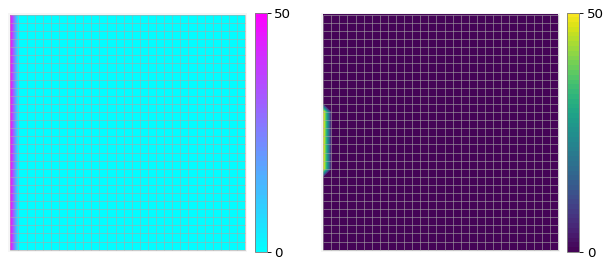
\includegraphics{07_Sol_Sis_Lin_Iter_1_files/figure-pdf/cell-12-output-1.png}

\bookmarksetup{startatroot}

\chapter{Método de Gauss-Seidel}\label{muxe9todo-de-gauss-seidel}

\begin{itemize}
\item
  La principal diferencia con el método de Jacobi es que las ecuaciones
  se analizan en un orden determinado.
\item
  Por ejemplo, si realizamos el cálculo en orden ascendente y ya hemos
  evaluado \(x_1\) y \(x_2\), para evaluar \(x_3\) haríamos lo
  siguiente:\} \[
  \begin{eqnarray*}
  \underline{x_1^1} & = &\left( b_1 - (a_{12}x_2^0 + a_{13} x_3^0 + \dots  + a_{1n}x_n^0) \right) / a_{11}  \\
  \underline{x_2^1} & = &\left( b_2 - (a_{21}\underline{x_1^1} + a_{23}x_3^0 + \dots  + a_{2n}x_n^0) \right) / a_{22} \\
  x_3 & = &\left( b_3 - (a_{31}\underline{x_1^1} + a_{32}\underline{x_2^1} + \dots  + a_{3n}x_n^0)\right) / a_{22}
  \end{eqnarray*}
  \]
\item
  En general la fórmula del método es como sigue: \$\$ x\_i\^{}k =
  \frac{1}{a_{i,i}} \left(b\_i - \sum\emph{\{j \textless{} i\} a}\{i,j\}
  \underline{x_j^{k}}
\item
  \sum\emph{\{j \textgreater{} i\} a}\{i,j\} x\_j\^{}\{k-1\} \right)
  \$\$
\item
  Este algoritmo es serial dado que cada componente depende de que las
  componentes previas se hayan calculado (\emph{desplazamientos
  sucesivos}).
\item
  El valor de la nueva iteración \(\mathbf{x}^k\) depende del orden en
  que se examinan las componentes. Si se cambia el orden, el valor de
  \(\mathbf{x}^k\) cambia.
\end{itemize}

\section{Algoritmo Gauss-Seidel.}\label{algoritmo-gauss-seidel.}

En general, podemos definir el siguiente algoritmo para el método de
Gauss-Seidel.

Se aplican los mismo comentarios que para el algoritmo de Jacobi.

\section{Implementación.}\label{implementaciuxf3n.-2}

\begin{Shaded}
\begin{Highlighting}[]
\KeywordTok{def}\NormalTok{ gauss\_seidel(A,b,tol,kmax,xi,yi):}
\NormalTok{    N }\OperatorTok{=} \BuiltInTok{len}\NormalTok{(b[}\DecValTok{0}\NormalTok{])}
\NormalTok{    xnew }\OperatorTok{=}\NormalTok{ np.zeros(N)}
\NormalTok{    xold }\OperatorTok{=}\NormalTok{ np.zeros(N)}
\NormalTok{    x }\OperatorTok{=}\NormalTok{ np.array([}\DecValTok{2}\NormalTok{, }\OperatorTok{{-}}\DecValTok{2}\NormalTok{]) }\CommentTok{\# Solución exacta}

    \CommentTok{\# Solución inicial}
\NormalTok{    xold[}\DecValTok{0}\NormalTok{] }\OperatorTok{=}\NormalTok{ xi}
\NormalTok{    xold[}\DecValTok{1}\NormalTok{] }\OperatorTok{=}\NormalTok{ yi}

\NormalTok{    xs }\OperatorTok{=}\NormalTok{ [xi]}
\NormalTok{    ys }\OperatorTok{=}\NormalTok{ [yi]}
    
\NormalTok{    e }\OperatorTok{=} \DecValTok{10}
\NormalTok{    error }\OperatorTok{=}\NormalTok{ [] }
    
\NormalTok{    k }\OperatorTok{=} \DecValTok{0}
    \BuiltInTok{print}\NormalTok{(}\StringTok{\textquotesingle{}}\SpecialCharTok{\{:\^{}2\}}\StringTok{ }\SpecialCharTok{\{:\^{}10\}}\StringTok{ }\SpecialCharTok{\{:\^{}12\}}\StringTok{ }\SpecialCharTok{\{:\^{}12\}}\StringTok{\textquotesingle{}}\NormalTok{.}\BuiltInTok{format}\NormalTok{(}\StringTok{\textquotesingle{} i \textquotesingle{}}\NormalTok{, }\StringTok{\textquotesingle{}Error\textquotesingle{}}\NormalTok{, }\StringTok{\textquotesingle{}x0\textquotesingle{}}\NormalTok{, }\StringTok{\textquotesingle{}x1\textquotesingle{}}\NormalTok{))}
    \ControlFlowTok{while}\NormalTok{(e }\OperatorTok{\textgreater{}}\NormalTok{ tol }\KeywordTok{and}\NormalTok{ k }\OperatorTok{\textless{}}\NormalTok{ kmax) :}
        \ControlFlowTok{for}\NormalTok{ i }\KeywordTok{in} \BuiltInTok{range}\NormalTok{(}\DecValTok{0}\NormalTok{,N): }\CommentTok{\# se puede hacer en paralelo}
\NormalTok{            xnew[i] }\OperatorTok{=} \DecValTok{0}
            \ControlFlowTok{for}\NormalTok{ j }\KeywordTok{in} \BuiltInTok{range}\NormalTok{(}\DecValTok{0}\NormalTok{,i):}
\NormalTok{                xnew[i] }\OperatorTok{+=}\NormalTok{ A[i,j] }\OperatorTok{*}\NormalTok{ xnew[j]}
            \ControlFlowTok{for}\NormalTok{ j }\KeywordTok{in} \BuiltInTok{range}\NormalTok{(i}\OperatorTok{+}\DecValTok{1}\NormalTok{,N):}
\NormalTok{                xnew[i] }\OperatorTok{+=}\NormalTok{ A[i,j] }\OperatorTok{*}\NormalTok{ xold[j]                }
\NormalTok{            xnew[i] }\OperatorTok{=}\NormalTok{ (b[}\DecValTok{0}\NormalTok{,i] }\OperatorTok{{-}}\NormalTok{ xnew[i]) }\OperatorTok{/}\NormalTok{ A[i,i]}
            
        \CommentTok{\# Almacenamos la solución actual}
\NormalTok{        xs.append(xnew[}\DecValTok{0}\NormalTok{])}
\NormalTok{        ys.append(xnew[}\DecValTok{1}\NormalTok{])}

\NormalTok{        e }\OperatorTok{=}\NormalTok{ np.linalg.norm(xnew}\OperatorTok{{-}}\NormalTok{x,}\DecValTok{2}\NormalTok{) }\CommentTok{\# Cálculo del error}
\NormalTok{        error.append(e)}
\NormalTok{        k }\OperatorTok{+=} \DecValTok{1}
\NormalTok{        xold[:] }\OperatorTok{=}\NormalTok{ xnew[:]}
        \BuiltInTok{print}\NormalTok{(}\StringTok{\textquotesingle{}}\SpecialCharTok{\{:2d\}}\StringTok{ }\SpecialCharTok{\{:10.9f\}}\StringTok{ (}\SpecialCharTok{\{:10.9f\}}\StringTok{, }\SpecialCharTok{\{:10.9f\}}\StringTok{)\textquotesingle{}}\NormalTok{.}\BuiltInTok{format}\NormalTok{(k, e, xnew[}\DecValTok{0}\NormalTok{], xnew[}\DecValTok{1}\NormalTok{]))}
    \ControlFlowTok{return}\NormalTok{ xnew, np.array(xs), np.array(ys), error, k}
\end{Highlighting}
\end{Shaded}

\section{\texorpdfstring{\textbf{Ejercicio
2.}}{Ejercicio 2.}}\label{ejercicio-2.-4}

Haciendo uso de la función \texttt{gauss\_seidel()} definida en la celda
anterior, aproxima la solución del sistema de ecuaciones del Ejemplo 1.
Utiliza la solución inicial \texttt{(xi,\ yi)\ =} \((-2, 2)\), una
tolerancia \texttt{tol} = \(1 \times 10^{-5}\) y \texttt{kmax} = \(50\)
iteraciones. Utiliza las variables \texttt{solG}, \texttt{xs},
\texttt{ys}, \texttt{eG} e \texttt{itG} para almacenar la salida de la
función \texttt{gauss\_seidel()}. Posteriormente grafica las rectas y
cómo se va calculando la solución con este método (puedes usar el mismo
código que en el caso de Jacobi). Grafica también los errores para el
método de Jacobi y para el de Gauss-Seidel, deberías obtener una imagen
como la siguiente:

\textbf{Cálculo de la solución con Gauss-Seidel}

\begin{Shaded}
\begin{Highlighting}[]
\CommentTok{\# Solución inicial}
\CommentTok{\# xi, yi = }
\CommentTok{\# tol = }
\CommentTok{\# kmax = }

\CommentTok{\# Método de Gauss{-}Seidel}
\CommentTok{\# ...}

\CommentTok{\#\#\# }\RegionMarkerTok{BEGIN}\CommentTok{ SOLUTION}
\CommentTok{\# Solución inicial}
\NormalTok{xi, yi }\OperatorTok{=} \OperatorTok{{-}}\DecValTok{2}\NormalTok{, }\DecValTok{2}
\NormalTok{tol }\OperatorTok{=} \FloatTok{1e{-}5}
\NormalTok{kmax }\OperatorTok{=} \DecValTok{50}

\CommentTok{\# Método de Gauss{-}Seidel}
\NormalTok{solG, xs, ys, eG, itG }\OperatorTok{=}\NormalTok{ gauss\_seidel(A, b, tol, kmax, xi, yi)}

\CommentTok{\#file\_answer.write(\textquotesingle{}4\textquotesingle{}, solG, \textquotesingle{}solG es incorrecta: revisa la llamada y ejecución de la función gauss\_seidel() así como sus parámetros de entrada.\textquotesingle{})}
\CommentTok{\#file\_answer.write(\textquotesingle{}5\textquotesingle{}, eG[{-}1], \textquotesingle{}eG[{-}1] es incorrecto: revisa la llamada y ejecución de la función gauss\_seidel() así como sus parámetros de entrada.\textquotesingle{})}
\CommentTok{\#file\_answer.write(\textquotesingle{}6\textquotesingle{}, itG, \textquotesingle{}itG es incorrector: revisa la llamada y ejecución de la función gauss\_seidel() así como sus parámetros de entrada.\textquotesingle{})}

\CommentTok{\#\#\# }\RegionMarkerTok{END}\CommentTok{ SOLUTION}
\end{Highlighting}
\end{Shaded}

\begin{verbatim}
 i    Error         x0           x1     
 1 2.810913476 (-0.666666667, -1.111111111)
 2 0.624647439 (1.407407407, -1.802469136)
 3 0.138810542 (1.868312757, -1.956104252)
 4 0.030846787 (1.970736168, -1.990245389)
 5 0.006854842 (1.993496926, -1.997832309)
 6 0.001523298 (1.998554873, -1.999518291)
 7 0.000338511 (1.999678861, -1.999892954)
 8 0.000075225 (1.999928636, -1.999976212)
 9 0.000016717 (1.999984141, -1.999994714)
10 0.000003715 (1.999996476, -1.999998825)
\end{verbatim}

\begin{Shaded}
\begin{Highlighting}[]
\CommentTok{\#quizz.eval\_numeric(\textquotesingle{}4\textquotesingle{}, solG)}
\CommentTok{\#quizz.eval\_numeric(\textquotesingle{}5\textquotesingle{}, eG[{-}1])}
\CommentTok{\#quizz.eval\_numeric(\textquotesingle{}6\textquotesingle{}, itG)}
\end{Highlighting}
\end{Shaded}

\textbf{Gráfica de las rectas, la solución y los pasos realizados}

\begin{Shaded}
\begin{Highlighting}[]
\CommentTok{\# Puedes usar el mismo código que en el caso anterior.}

\CommentTok{\#\#\# }\RegionMarkerTok{BEGIN}\CommentTok{ SOLUTION}
\NormalTok{v }\OperatorTok{=}\NormalTok{ mvis.Plotter(}\DecValTok{1}\NormalTok{,}\DecValTok{1}\NormalTok{,[}\BuiltInTok{dict}\NormalTok{(aspect}\OperatorTok{=}\StringTok{\textquotesingle{}equal\textquotesingle{}}\NormalTok{)],title}\OperatorTok{=}\StringTok{\textquotesingle{}Cruce de rectas\textquotesingle{}}\NormalTok{) }
\NormalTok{v.set\_coordsys(}\DecValTok{1}\NormalTok{)}
\NormalTok{v.plot(}\DecValTok{1}\NormalTok{, x, y1, lw }\OperatorTok{=} \DecValTok{3}\NormalTok{, c }\OperatorTok{=} \StringTok{\textquotesingle{}seagreen\textquotesingle{}}\NormalTok{, label }\OperatorTok{=} \StringTok{\textquotesingle{}$3x+2y=2$\textquotesingle{}}\NormalTok{) }\CommentTok{\# Línea recta 1}
\NormalTok{v.plot(}\DecValTok{1}\NormalTok{, x, y2, lw }\OperatorTok{=} \DecValTok{3}\NormalTok{, c }\OperatorTok{=} \StringTok{\textquotesingle{}mediumorchid\textquotesingle{}}\NormalTok{, label }\OperatorTok{=} \StringTok{\textquotesingle{}$2x+6y={-}8$\textquotesingle{}}\NormalTok{) }\CommentTok{\# Línea recta 2}

\CommentTok{\# Graficamos los pasos}
\NormalTok{v.scatter(}\DecValTok{1}\NormalTok{, xs[}\DecValTok{0}\NormalTok{], ys[}\DecValTok{0}\NormalTok{], fc}\OperatorTok{=}\StringTok{\textquotesingle{}yellow\textquotesingle{}}\NormalTok{, ec}\OperatorTok{=}\StringTok{\textquotesingle{}k\textquotesingle{}}\NormalTok{, s }\OperatorTok{=} \DecValTok{75}\NormalTok{, alpha}\OperatorTok{=}\FloatTok{0.75}\NormalTok{, zorder}\OperatorTok{=}\DecValTok{8}\NormalTok{, label}\OperatorTok{=}\StringTok{\textquotesingle{}Sol. inicial\textquotesingle{}}\NormalTok{)}
\NormalTok{v.scatter(}\DecValTok{1}\NormalTok{, xs[}\DecValTok{1}\NormalTok{:], ys[}\DecValTok{1}\NormalTok{:], c}\OperatorTok{=}\StringTok{\textquotesingle{}navy\textquotesingle{}}\NormalTok{, s }\OperatorTok{=} \DecValTok{10}\NormalTok{, alpha}\OperatorTok{=}\FloatTok{0.5}\NormalTok{, zorder}\OperatorTok{=}\DecValTok{8}\NormalTok{)}
\NormalTok{v.plot(}\DecValTok{1}\NormalTok{, xs, ys, c}\OperatorTok{=}\StringTok{\textquotesingle{}grey\textquotesingle{}}\NormalTok{, ls }\OperatorTok{=} \StringTok{\textquotesingle{}{-}{-}\textquotesingle{}}\NormalTok{, lw}\OperatorTok{=}\FloatTok{1.0}\NormalTok{, zorder}\OperatorTok{=}\DecValTok{8}\NormalTok{, label}\OperatorTok{=}\StringTok{\textquotesingle{}Pasos de Gauss{-}Seidel\textquotesingle{}}\NormalTok{)}

\NormalTok{v.legend(ncol }\OperatorTok{=} \DecValTok{1}\NormalTok{, frameon}\OperatorTok{=}\VariableTok{True}\NormalTok{, loc}\OperatorTok{=}\StringTok{\textquotesingle{}best\textquotesingle{}}\NormalTok{, bbox\_to\_anchor}\OperatorTok{=}\NormalTok{(}\FloatTok{2.05}\NormalTok{, }\FloatTok{1.01}\NormalTok{))}
\NormalTok{v.grid()}
\NormalTok{v.show()}
\CommentTok{\#\#\# }\RegionMarkerTok{END}\CommentTok{ SOLUTION}
\end{Highlighting}
\end{Shaded}

\includegraphics{07_Sol_Sis_Lin_Iter_1_files/figure-pdf/cell-16-output-1.png}

\textbf{Graficación de los errores de Jacobi y Gauss-Seidel}

\begin{Shaded}
\begin{Highlighting}[]
\CommentTok{\# Utiliza el código del caso anterior adaptado para que pueda graficar ambos errores.}

\CommentTok{\#\#\# }\RegionMarkerTok{BEGIN}\CommentTok{ SOLUTION}
\CommentTok{\# Lista con el número de las iteraciones máxima}
\NormalTok{it\_max }\OperatorTok{=} \BuiltInTok{max}\NormalTok{(itJ, itG)}\OperatorTok{+}\DecValTok{1}
\NormalTok{l\_it\_max }\OperatorTok{=} \BuiltInTok{list}\NormalTok{(}\BuiltInTok{range}\NormalTok{(}\DecValTok{1}\NormalTok{,it\_max)) }

\CommentTok{\# Listas con el número de las iteraciones para cada algoritmo}
\NormalTok{l\_itJ }\OperatorTok{=} \BuiltInTok{list}\NormalTok{(}\BuiltInTok{range}\NormalTok{(}\DecValTok{1}\NormalTok{,itJ}\OperatorTok{+}\DecValTok{1}\NormalTok{)) }
\NormalTok{l\_itG }\OperatorTok{=} \BuiltInTok{list}\NormalTok{(}\BuiltInTok{range}\NormalTok{(}\DecValTok{1}\NormalTok{,itG}\OperatorTok{+}\DecValTok{1}\NormalTok{)) }

\CommentTok{\# Parámetros para los ejes}
\NormalTok{a\_p }\OperatorTok{=} \BuiltInTok{dict}\NormalTok{(yscale}\OperatorTok{=}\StringTok{\textquotesingle{}log\textquotesingle{}}\NormalTok{, xlabel}\OperatorTok{=}\StringTok{\textquotesingle{}Iteraciones\textquotesingle{}}\NormalTok{, xticks }\OperatorTok{=}\NormalTok{ l\_it\_max)}

\CommentTok{\# Gráficas del error}
\NormalTok{v }\OperatorTok{=}\NormalTok{ mvis.Plotter(}\DecValTok{1}\NormalTok{,}\DecValTok{1}\NormalTok{,[a\_p]) }
\NormalTok{v.axes(}\DecValTok{1}\NormalTok{).set\_title(}\StringTok{\textquotesingle{}Error\textquotesingle{}}\NormalTok{, loc}\OperatorTok{=}\StringTok{\textquotesingle{}left\textquotesingle{}}\NormalTok{)}
\NormalTok{v.plot(}\DecValTok{1}\NormalTok{, l\_itJ, eJ, marker}\OperatorTok{=}\StringTok{\textquotesingle{}.\textquotesingle{}}\NormalTok{, label}\OperatorTok{=}\StringTok{\textquotesingle{}Jacobi\textquotesingle{}}\NormalTok{)}
\NormalTok{v.plot(}\DecValTok{1}\NormalTok{, l\_itG, eG, marker}\OperatorTok{=}\StringTok{\textquotesingle{}.\textquotesingle{}}\NormalTok{, label}\OperatorTok{=}\StringTok{\textquotesingle{}Gauss{-}Seidel\textquotesingle{}}\NormalTok{)}
\NormalTok{v.legend()}
\NormalTok{v.grid()}
\CommentTok{\#\#\# }\RegionMarkerTok{END}\CommentTok{ SOLUTION}
\end{Highlighting}
\end{Shaded}

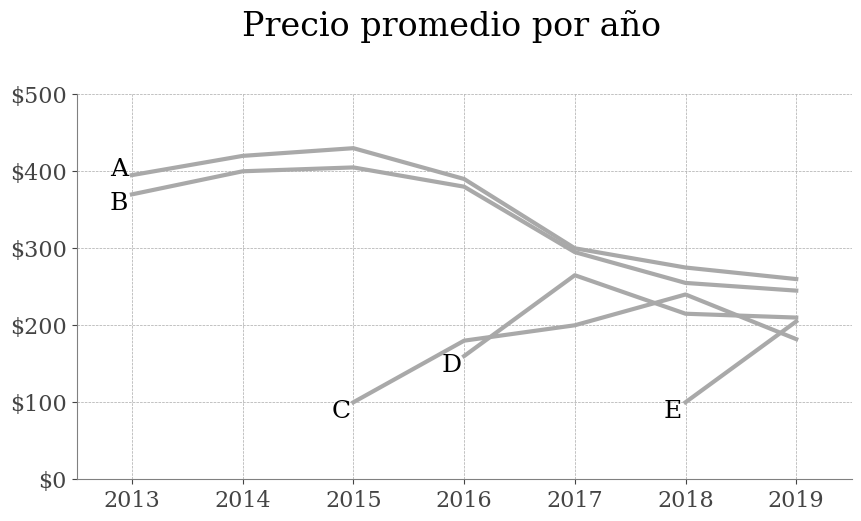
\includegraphics{07_Sol_Sis_Lin_Iter_1_files/figure-pdf/cell-17-output-1.png}

\bookmarksetup{startatroot}

\chapter{\texorpdfstring{Método de Sobrerrelajación sucesiva
(\emph{Successive Overrelaxation},
SOR)}{Método de Sobrerrelajación sucesiva (Successive Overrelaxation, SOR)}}\label{muxe9todo-de-sobrerrelajaciuxf3n-sucesiva-successive-overrelaxation-sor}

\begin{itemize}
\item
  Se obtiene apicando una extrapolación a la iteración de Gauss-Seidel.
\item
  Esta extrapolación es un promedio pesado entre la iteración actual y
  la anterior: \[
  x_i^k = \omega \bar{x}_i^k + (1-\omega)x_i^{k-1}
  \] donde \(\bar{x}\) denota una iteración de Gauss-Seidel y \(\omega\)
  es el factor de extrapolación.
\item
  En términos de matrices tenemos: \$\$ \mathbf{x}\^{}k = (\mathbf{D} -
  \omega \mathbf{L})\^{}\{-1\}(\omega \mathbf{U} + (1 -
  \omega )\mathbf{D})\mathbf{x}\^{}\{k-1\}
\item
  \omega (\mathbf{D} - \omega \mathbf{L})\^{}\{-1\} \mathbf{b} \$\$
\item
  Elegir la \(\omega\) óptima no es simple, aunque se sabe que si
  \(\omega\) está fuera del intervalo \((0,2)\) el método falla.
\end{itemize}

\section{Implementación 3.}\label{implementaciuxf3n-3.}

\begin{Shaded}
\begin{Highlighting}[]
\KeywordTok{def}\NormalTok{ sor(A,b,tol,kmax,w,xi,yi):}
\NormalTok{    N }\OperatorTok{=} \BuiltInTok{len}\NormalTok{(b[}\DecValTok{0}\NormalTok{])}
\NormalTok{    xnew }\OperatorTok{=}\NormalTok{ np.zeros(N)}
\NormalTok{    xold }\OperatorTok{=}\NormalTok{ np.zeros(N)}
\NormalTok{    x }\OperatorTok{=}\NormalTok{ np.array([}\DecValTok{2}\NormalTok{, }\OperatorTok{{-}}\DecValTok{2}\NormalTok{]) }\CommentTok{\# Solución exacta}

    \CommentTok{\# Solución inicial}
\NormalTok{    xold[}\DecValTok{0}\NormalTok{] }\OperatorTok{=}\NormalTok{ xi}
\NormalTok{    xold[}\DecValTok{1}\NormalTok{] }\OperatorTok{=}\NormalTok{ yi}

\NormalTok{    xs }\OperatorTok{=}\NormalTok{ [xi]}
\NormalTok{    ys }\OperatorTok{=}\NormalTok{ [yi]}
    
\NormalTok{    e }\OperatorTok{=} \DecValTok{10}
\NormalTok{    error }\OperatorTok{=}\NormalTok{ [] }
    
\NormalTok{    k }\OperatorTok{=} \DecValTok{0}
    \ControlFlowTok{while}\NormalTok{(e }\OperatorTok{\textgreater{}}\NormalTok{ tol }\KeywordTok{and}\NormalTok{ k }\OperatorTok{\textless{}}\NormalTok{ kmax) :}
        \ControlFlowTok{for}\NormalTok{ i }\KeywordTok{in} \BuiltInTok{range}\NormalTok{(}\DecValTok{0}\NormalTok{,N): }\CommentTok{\# se puede hacer en paralelo}
\NormalTok{            sigma }\OperatorTok{=} \DecValTok{0}
            \ControlFlowTok{for}\NormalTok{ j }\KeywordTok{in} \BuiltInTok{range}\NormalTok{(}\DecValTok{0}\NormalTok{,i):}
\NormalTok{                sigma }\OperatorTok{+=}\NormalTok{ A[i,j] }\OperatorTok{*}\NormalTok{ xnew[j]}
            \ControlFlowTok{for}\NormalTok{ j }\KeywordTok{in} \BuiltInTok{range}\NormalTok{(i}\OperatorTok{+}\DecValTok{1}\NormalTok{,N):}
\NormalTok{                sigma }\OperatorTok{+=}\NormalTok{ A[i,j] }\OperatorTok{*}\NormalTok{ xold[j]                }
\NormalTok{            sigma }\OperatorTok{=}\NormalTok{ (b[}\DecValTok{0}\NormalTok{,i] }\OperatorTok{{-}}\NormalTok{ sigma) }\OperatorTok{/}\NormalTok{ A[i,i]}
\NormalTok{            xnew[i] }\OperatorTok{=}\NormalTok{ xold[i] }\OperatorTok{+}\NormalTok{ w }\OperatorTok{*}\NormalTok{ (sigma }\OperatorTok{{-}}\NormalTok{xold[i])}
            
        \CommentTok{\# Almacenamos la solución actual}
\NormalTok{        xs.append(xnew[}\DecValTok{0}\NormalTok{])}
\NormalTok{        ys.append(xnew[}\DecValTok{1}\NormalTok{])}
        
\NormalTok{        e }\OperatorTok{=}\NormalTok{ np.linalg.norm(xnew}\OperatorTok{{-}}\NormalTok{x, }\DecValTok{2}\NormalTok{) }\CommentTok{\# Cálculo del error}
\NormalTok{        error.append(e)}
\NormalTok{        k }\OperatorTok{+=} \DecValTok{1}
\NormalTok{        xold[:] }\OperatorTok{=}\NormalTok{ xnew[:]}
        \BuiltInTok{print}\NormalTok{(}\StringTok{\textquotesingle{}}\SpecialCharTok{\{:2d\}}\StringTok{ }\SpecialCharTok{\{:10.9f\}}\StringTok{ (}\SpecialCharTok{\{:10.9f\}}\StringTok{, }\SpecialCharTok{\{:10.9f\}}\StringTok{)\textquotesingle{}}\NormalTok{.}\BuiltInTok{format}\NormalTok{(k, e, xnew[}\DecValTok{0}\NormalTok{], xnew[}\DecValTok{1}\NormalTok{]))}
    \ControlFlowTok{return}\NormalTok{ xnew, np.array(xs), np.array(ys), error, k}
\end{Highlighting}
\end{Shaded}

\section{\texorpdfstring{\textbf{Ejercicio
3.}}{Ejercicio 3.}}\label{ejercicio-3.-2}

Haciendo uso de la función \texttt{sor()} definida en la celda anterior,
aproxima la solución del sistema de ecuaciones del Ejercicio 1. Utiliza
la solución inicial \texttt{(xi,\ yi)\ =} \((-2, 2)\), una tolerancia
\texttt{tol} = \(1 \times 10^{-5}\) y \texttt{kmax} = \(50\)
iteraciones. Elije el valor de \(\omega = 1.09\). Utiliza las variables
\texttt{solSOR}, \texttt{xs}, \texttt{ys}, \texttt{eSOR} e
\texttt{itSOR} para almacenar la salida de la función
\texttt{gauss\_seidel()}. Posteriormente grafica las rectas y cómo se va
calculando la solución con este método (puedes usar el mismo código que
en el caso de Jacobi). Grafica también los errores para los tres métodos
(Jacobi, Gauss-Seidel y SOR).

\textbf{Cálculo de la solución con SOR}

\begin{Shaded}
\begin{Highlighting}[]
\CommentTok{\# Solución inicial}
\CommentTok{\# xi, yi = }
\CommentTok{\# tol = }
\CommentTok{\# kmax = }

\CommentTok{\# Método de SOR, probar con w = 1.09, 1.8, 1.99, 2.0}
\CommentTok{\# w = ...}
\CommentTok{\# ...}

\CommentTok{\#\#\# }\RegionMarkerTok{BEGIN}\CommentTok{ SOLUTION}
\CommentTok{\# Solución inicial}
\NormalTok{xi, yi }\OperatorTok{=} \OperatorTok{{-}}\DecValTok{2}\NormalTok{, }\DecValTok{2}
\NormalTok{tol }\OperatorTok{=} \FloatTok{1e{-}5}
\NormalTok{kmax }\OperatorTok{=} \DecValTok{50}

\CommentTok{\# Método de SOR, probar con w = 1.09, 1.8, 1.99, 2.0}
\NormalTok{w }\OperatorTok{=} \FloatTok{1.09}
\NormalTok{solSOR, xs, ys, eSOR, itSOR }\OperatorTok{=}\NormalTok{ sor(A, b, tol, kmax, w, xi, yi)}

\CommentTok{\#file\_answer.write(\textquotesingle{}7\textquotesingle{}, solSOR, \textquotesingle{}solSOR es incorrecta: revisa la llamada y ejecución de la función sor() así como sus parámetros de entrada.\textquotesingle{})}
\CommentTok{\#file\_answer.write(\textquotesingle{}8\textquotesingle{}, eSOR[{-}1], \textquotesingle{}eSOR[{-}1] es incorrecto: revisa la llamada y ejecución de la función sor() así como sus parámetros de entrada.\textquotesingle{})}
\CommentTok{\#file\_answer.write(\textquotesingle{}9\textquotesingle{}, itSOR, \textquotesingle{}itSOR es incorrector: revisa la llamada y ejecución de la función sor() así como sus parámetros de entrada.\textquotesingle{})}

\CommentTok{\#\#\# }\RegionMarkerTok{END}\CommentTok{ SOLUTION}
\end{Highlighting}
\end{Shaded}

\begin{verbatim}
 1 2.608651498 (-0.546666667, -1.434711111)
 2 0.182203110 (1.818423407, -1.984903171)
 3 0.006309667 (2.005371531, -2.003310371)
 4 0.001963366 (2.001922098, -2.000400429)
 5 0.000118187 (2.000117990, -2.000006831)
 6 0.000006254 (1.999994345, -1.999997330)
\end{verbatim}

\begin{Shaded}
\begin{Highlighting}[]
\CommentTok{\#quizz.eval\_numeric(\textquotesingle{}7\textquotesingle{}, solSOR)}
\CommentTok{\#quizz.eval\_numeric(\textquotesingle{}8\textquotesingle{}, eSOR[{-}1])}
\CommentTok{\#quizz.eval\_numeric(\textquotesingle{}9\textquotesingle{}, itSOR)}
\end{Highlighting}
\end{Shaded}

\textbf{Gráfica de las rectas, la solución y los pasos realizados}

\begin{Shaded}
\begin{Highlighting}[]
\CommentTok{\# Puedes usar el mismo código que en el caso anterior.}

\CommentTok{\#\#\# }\RegionMarkerTok{BEGIN}\CommentTok{ SOLUTION}
\NormalTok{v }\OperatorTok{=}\NormalTok{ mvis.Plotter(}\DecValTok{1}\NormalTok{,}\DecValTok{1}\NormalTok{,[}\BuiltInTok{dict}\NormalTok{(aspect}\OperatorTok{=}\StringTok{\textquotesingle{}equal\textquotesingle{}}\NormalTok{)],title}\OperatorTok{=}\StringTok{\textquotesingle{}Cruce de rectas\textquotesingle{}}\NormalTok{) }
\NormalTok{v.set\_coordsys(}\DecValTok{1}\NormalTok{)}
\NormalTok{v.plot(}\DecValTok{1}\NormalTok{, x, y1, lw }\OperatorTok{=} \DecValTok{3}\NormalTok{, c }\OperatorTok{=} \StringTok{\textquotesingle{}seagreen\textquotesingle{}}\NormalTok{, label }\OperatorTok{=} \StringTok{\textquotesingle{}$3x+2y=2$\textquotesingle{}}\NormalTok{) }\CommentTok{\# Línea recta 1}
\NormalTok{v.plot(}\DecValTok{1}\NormalTok{, x, y2, lw }\OperatorTok{=} \DecValTok{3}\NormalTok{, c }\OperatorTok{=} \StringTok{\textquotesingle{}mediumorchid\textquotesingle{}}\NormalTok{, label }\OperatorTok{=} \StringTok{\textquotesingle{}$2x+6y={-}8$\textquotesingle{}}\NormalTok{) }\CommentTok{\# Línea recta 2}
\NormalTok{v.scatter(}\DecValTok{1}\NormalTok{, sol[}\DecValTok{0}\NormalTok{], sol[}\DecValTok{1}\NormalTok{], fc}\OperatorTok{=}\StringTok{\textquotesingle{}sandybrown\textquotesingle{}}\NormalTok{, ec}\OperatorTok{=}\StringTok{\textquotesingle{}k\textquotesingle{}}\NormalTok{, s }\OperatorTok{=} \DecValTok{75}\NormalTok{, alpha}\OperatorTok{=}\FloatTok{0.75}\NormalTok{, zorder}\OperatorTok{=}\DecValTok{5}\NormalTok{, label}\OperatorTok{=}\StringTok{\textquotesingle{}Sol. final\textquotesingle{}}\NormalTok{) }\CommentTok{\# Solución}

\CommentTok{\# Graficamos los pasos}
\NormalTok{v.scatter(}\DecValTok{1}\NormalTok{, xs[}\DecValTok{0}\NormalTok{], ys[}\DecValTok{0}\NormalTok{], fc}\OperatorTok{=}\StringTok{\textquotesingle{}yellow\textquotesingle{}}\NormalTok{, ec}\OperatorTok{=}\StringTok{\textquotesingle{}k\textquotesingle{}}\NormalTok{, s }\OperatorTok{=} \DecValTok{75}\NormalTok{, alpha}\OperatorTok{=}\FloatTok{0.75}\NormalTok{, zorder}\OperatorTok{=}\DecValTok{8}\NormalTok{, label}\OperatorTok{=}\StringTok{\textquotesingle{}Sol. inicial\textquotesingle{}}\NormalTok{)}
\NormalTok{v.scatter(}\DecValTok{1}\NormalTok{, xs[}\DecValTok{1}\NormalTok{:], ys[}\DecValTok{1}\NormalTok{:], c}\OperatorTok{=}\StringTok{\textquotesingle{}navy\textquotesingle{}}\NormalTok{, s }\OperatorTok{=} \DecValTok{10}\NormalTok{, alpha}\OperatorTok{=}\FloatTok{0.5}\NormalTok{, zorder}\OperatorTok{=}\DecValTok{8}\NormalTok{)}
\NormalTok{v.plot(}\DecValTok{1}\NormalTok{, xs, ys, c}\OperatorTok{=}\StringTok{\textquotesingle{}grey\textquotesingle{}}\NormalTok{, ls }\OperatorTok{=} \StringTok{\textquotesingle{}{-}{-}\textquotesingle{}}\NormalTok{, lw}\OperatorTok{=}\FloatTok{1.0}\NormalTok{, zorder}\OperatorTok{=}\DecValTok{8}\NormalTok{, label}\OperatorTok{=}\StringTok{\textquotesingle{}Pasos del SOR\textquotesingle{}}\NormalTok{)}
        
\NormalTok{v.legend(ncol }\OperatorTok{=} \DecValTok{1}\NormalTok{, frameon}\OperatorTok{=}\VariableTok{True}\NormalTok{, loc}\OperatorTok{=}\StringTok{\textquotesingle{}best\textquotesingle{}}\NormalTok{, bbox\_to\_anchor}\OperatorTok{=}\NormalTok{(}\FloatTok{1.78}\NormalTok{, }\FloatTok{1.01}\NormalTok{))}
\NormalTok{v.grid()}
\NormalTok{v.show()}
\CommentTok{\#\#\# }\RegionMarkerTok{END}\CommentTok{ SOLUTION}
\end{Highlighting}
\end{Shaded}

\includegraphics{07_Sol_Sis_Lin_Iter_1_files/figure-pdf/cell-21-output-1.png}

\begin{Shaded}
\begin{Highlighting}[]
\CommentTok{\# Utiliza el código del caso anterior adaptado para que pueda graficar los tres errores.}

\CommentTok{\#\#\# }\RegionMarkerTok{BEGIN}\CommentTok{ SOLUTION}
\CommentTok{\# Lista con el número de las iteraciones máxima}
\NormalTok{it\_max }\OperatorTok{=} \BuiltInTok{max}\NormalTok{(itJ, itG, itSOR)}\OperatorTok{+}\DecValTok{1}
\NormalTok{l\_it\_max }\OperatorTok{=} \BuiltInTok{list}\NormalTok{(}\BuiltInTok{range}\NormalTok{(}\DecValTok{1}\NormalTok{,it\_max)) }

\CommentTok{\# Listas con el número de las iteraciones para cada algoritmo}
\NormalTok{l\_itJ }\OperatorTok{=} \BuiltInTok{list}\NormalTok{(}\BuiltInTok{range}\NormalTok{(}\DecValTok{1}\NormalTok{,itJ}\OperatorTok{+}\DecValTok{1}\NormalTok{)) }
\NormalTok{l\_itG }\OperatorTok{=} \BuiltInTok{list}\NormalTok{(}\BuiltInTok{range}\NormalTok{(}\DecValTok{1}\NormalTok{,itG}\OperatorTok{+}\DecValTok{1}\NormalTok{)) }
\NormalTok{l\_itSOR }\OperatorTok{=} \BuiltInTok{list}\NormalTok{(}\BuiltInTok{range}\NormalTok{(}\DecValTok{1}\NormalTok{,itSOR}\OperatorTok{+}\DecValTok{1}\NormalTok{)) }

\CommentTok{\# Parámetros para los ejes}
\NormalTok{a\_p }\OperatorTok{=} \BuiltInTok{dict}\NormalTok{(yscale}\OperatorTok{=}\StringTok{\textquotesingle{}log\textquotesingle{}}\NormalTok{, xlabel}\OperatorTok{=}\StringTok{\textquotesingle{}Iteraciones\textquotesingle{}}\NormalTok{, xticks }\OperatorTok{=}\NormalTok{ l\_it\_max)}

\CommentTok{\# Gráficas del error}
\NormalTok{v }\OperatorTok{=}\NormalTok{ mvis.Plotter(}\DecValTok{1}\NormalTok{,}\DecValTok{1}\NormalTok{,[a\_p]) }
\NormalTok{v.axes(}\DecValTok{1}\NormalTok{).set\_title(}\StringTok{\textquotesingle{}Error\textquotesingle{}}\NormalTok{, loc}\OperatorTok{=}\StringTok{\textquotesingle{}left\textquotesingle{}}\NormalTok{)}
\NormalTok{v.plot(}\DecValTok{1}\NormalTok{, l\_itJ, eJ, marker}\OperatorTok{=}\StringTok{\textquotesingle{}.\textquotesingle{}}\NormalTok{, label}\OperatorTok{=}\StringTok{\textquotesingle{}Jacobi\textquotesingle{}}\NormalTok{)}
\NormalTok{v.plot(}\DecValTok{1}\NormalTok{, l\_itG, eG, marker}\OperatorTok{=}\StringTok{\textquotesingle{}.\textquotesingle{}}\NormalTok{, label}\OperatorTok{=}\StringTok{\textquotesingle{}Gauss{-}Seidel\textquotesingle{}}\NormalTok{)}
\NormalTok{v.plot(}\DecValTok{1}\NormalTok{, l\_itSOR, eSOR, marker}\OperatorTok{=}\StringTok{\textquotesingle{}.\textquotesingle{}}\NormalTok{, label}\OperatorTok{=}\StringTok{\textquotesingle{}SOR\textquotesingle{}}\NormalTok{)}
\NormalTok{v.legend()}
\NormalTok{v.grid()}
\CommentTok{\#\#\# }\RegionMarkerTok{END}\CommentTok{ SOLUTION}
\end{Highlighting}
\end{Shaded}

\includegraphics{07_Sol_Sis_Lin_Iter_1_files/figure-pdf/cell-22-output-1.png}

\section{\texorpdfstring{\textbf{Ejercicio
4.}}{Ejercicio 4.}}\label{ejercicio-4.}

Almacena los errores de los tres métodos en los archivos:
\texttt{errorJacobi.npy}, \texttt{errorGaussSeidel.npy} y
\texttt{errorSOR.npy} usando la función \texttt{np.save()}, checa la
documentación
\href{https://numpy.org/doc/stable/reference/generated/numpy.save.html}{aquí}.

Prueba que tu código funciona usando:

\begin{verbatim}
print('Error Jacobi = \n{}\n'.format(np.load('errorJacobi.npy')))
print('Error Gauss-Seidel = \n{}\n'.format(np.load('errorGaussSeidel.npy')))
print('Error SOR = \n{}\n'.format(np.load('errorSOR.npy')))
\end{verbatim}

La salida debería ser:

\begin{verbatim}
Error Jacobi = 
[2.98142397e+00 1.25707872e+00 ...]

Error Gauss-Seidel = 
[2.81091348e+00 6.24647439e-01 ...]

Error SOR = 
[2.60865150e+00 1.82203110e-01 ...]
\end{verbatim}

\begin{Shaded}
\begin{Highlighting}[]
\CommentTok{\# np.save( ... )}
\CommentTok{\#}

\CommentTok{\#\#\# }\RegionMarkerTok{BEGIN}\CommentTok{ SOLUTION}
\NormalTok{np.save(}\StringTok{\textquotesingle{}errorJacobi.npy\textquotesingle{}}\NormalTok{,eJ)}
\NormalTok{np.save(}\StringTok{\textquotesingle{}errorGaussSeidel.npy\textquotesingle{}}\NormalTok{, eG)}
\NormalTok{np.save(}\StringTok{\textquotesingle{}errorSOR.npy\textquotesingle{}}\NormalTok{, eSOR)}
\CommentTok{\#\#\# }\RegionMarkerTok{END}\CommentTok{ SOLUTION}
\end{Highlighting}
\end{Shaded}

\begin{Shaded}
\begin{Highlighting}[]
\BuiltInTok{print}\NormalTok{(}\StringTok{\textquotesingle{}Error Jacobi = }\CharTok{\textbackslash{}n}\SpecialCharTok{\{\}}\CharTok{\textbackslash{}n}\StringTok{\textquotesingle{}}\NormalTok{.}\BuiltInTok{format}\NormalTok{(np.load(}\StringTok{\textquotesingle{}errorJacobi.npy\textquotesingle{}}\NormalTok{)))}
\BuiltInTok{print}\NormalTok{(}\StringTok{\textquotesingle{}Error Gauss{-}Seidel = }\CharTok{\textbackslash{}n}\SpecialCharTok{\{\}}\CharTok{\textbackslash{}n}\StringTok{\textquotesingle{}}\NormalTok{.}\BuiltInTok{format}\NormalTok{(np.load(}\StringTok{\textquotesingle{}errorGaussSeidel.npy\textquotesingle{}}\NormalTok{)))}
\BuiltInTok{print}\NormalTok{(}\StringTok{\textquotesingle{}Error SOR = }\CharTok{\textbackslash{}n}\SpecialCharTok{\{\}}\CharTok{\textbackslash{}n}\StringTok{\textquotesingle{}}\NormalTok{.}\BuiltInTok{format}\NormalTok{(np.load(}\StringTok{\textquotesingle{}errorSOR.npy\textquotesingle{}}\NormalTok{)))}
\end{Highlighting}
\end{Shaded}

\begin{verbatim}
Error Jacobi = 
[2.98142397e+00 1.25707872e+00 6.62538660e-01 2.79350827e-01
 1.47230813e-01 6.20779616e-02 3.27179585e-02 1.37951026e-02
 7.27065745e-03 3.06557835e-03 1.61570166e-03 6.81239633e-04
 3.59044812e-04 1.51386585e-04 7.97877361e-05 3.36414634e-05
 1.77306080e-05 7.47588075e-06]

Error Gauss-Seidel = 
[2.81091348e+00 6.24647439e-01 1.38810542e-01 3.08467871e-02
 6.85484158e-03 1.52329813e-03 3.38510695e-04 7.52245990e-05
 1.67165775e-05 3.71479501e-06]

Error SOR = 
[2.60865150e+00 1.82203110e-01 6.30966741e-03 1.96336589e-03
 1.18187146e-04 6.25365681e-06]
\end{verbatim}

\bookmarksetup{startatroot}

\chapter{Descenso del gradiente y Gradiente
Conjugado.}\label{descenso-del-gradiente-y-gradiente-conjugado.}

\textbf{Objetivo.}

Describir e implementar los métodos de descenso del gradiente y de
gradiente conjugado para la solución de sistemas de ecuaciones lineales.

MACTI-Algebra\_Lineal\_01 by Luis M. de la Cruz is licensed under
Attribution-ShareAlike 4.0 International

Trabajo realizado con el apoyo del Programa UNAM-DGAPA-PAPIME PE101922

\begin{Shaded}
\begin{Highlighting}[]
\ImportTok{import}\NormalTok{ numpy }\ImportTok{as}\NormalTok{ np}
\ImportTok{import}\NormalTok{ ipywidgets }\ImportTok{as}\NormalTok{ widgets}
\ImportTok{import}\NormalTok{ macti.visual }\ImportTok{as}\NormalTok{ mvis}
\ImportTok{import}\NormalTok{ macti.matem }\ImportTok{as}\NormalTok{ mmat}
\end{Highlighting}
\end{Shaded}

La siguiente función será usada para graficar algunos resultados.

\begin{Shaded}
\begin{Highlighting}[]
\KeywordTok{def}\NormalTok{ grafica(x, y1, y2, sol }\OperatorTok{=}\NormalTok{ [], xs }\OperatorTok{=}\NormalTok{ [], ys }\OperatorTok{=}\NormalTok{ [], vA }\OperatorTok{=}\NormalTok{ [], xg }\OperatorTok{=}\NormalTok{ [], yg }\OperatorTok{=}\NormalTok{ [], z }\OperatorTok{=}\NormalTok{ []):}
    \CommentTok{"""}
\CommentTok{    Esta función grafica las líneas rectas, la solución, los pasos y los eigenvectores.}
\CommentTok{    """}
\NormalTok{    v }\OperatorTok{=}\NormalTok{ mvis.Plotter(}\DecValTok{1}\NormalTok{,}\DecValTok{1}\NormalTok{,[}\BuiltInTok{dict}\NormalTok{(aspect}\OperatorTok{=}\StringTok{\textquotesingle{}equal\textquotesingle{}}\NormalTok{)],title}\OperatorTok{=}\StringTok{\textquotesingle{}Cruce de rectas\textquotesingle{}}\NormalTok{) }
\NormalTok{    v.set\_coordsys(}\DecValTok{1}\NormalTok{)}
    
    \CommentTok{\# Graficamos las líneas rectas}
\NormalTok{    v.plot(}\DecValTok{1}\NormalTok{, x, y1, lw }\OperatorTok{=} \DecValTok{3}\NormalTok{, c }\OperatorTok{=} \StringTok{\textquotesingle{}seagreen\textquotesingle{}}\NormalTok{, label }\OperatorTok{=} \StringTok{\textquotesingle{}$3x+2y=2$\textquotesingle{}}\NormalTok{) }\CommentTok{\# Línea recta 1}
\NormalTok{    v.plot(}\DecValTok{1}\NormalTok{, x, y2, lw }\OperatorTok{=} \DecValTok{3}\NormalTok{, c }\OperatorTok{=} \StringTok{\textquotesingle{}mediumorchid\textquotesingle{}}\NormalTok{, label }\OperatorTok{=} \StringTok{\textquotesingle{}$2x+6y={-}8$\textquotesingle{}}\NormalTok{) }\CommentTok{\# Línea recta 2}

    \ControlFlowTok{if} \BuiltInTok{len}\NormalTok{(sol):}
        \CommentTok{\# Graficamos la solución}
\NormalTok{        v.scatter(}\DecValTok{1}\NormalTok{, sol[}\DecValTok{0}\NormalTok{], sol[}\DecValTok{1}\NormalTok{], fc}\OperatorTok{=}\StringTok{\textquotesingle{}sandybrown\textquotesingle{}}\NormalTok{, ec}\OperatorTok{=}\StringTok{\textquotesingle{}k\textquotesingle{}}\NormalTok{, s }\OperatorTok{=} \DecValTok{75}\NormalTok{, alpha}\OperatorTok{=}\FloatTok{0.75}\NormalTok{, zorder}\OperatorTok{=}\DecValTok{5}\NormalTok{, label}\OperatorTok{=}\StringTok{\textquotesingle{}Solución final         .\textquotesingle{}}\NormalTok{) }\CommentTok{\# Solución}

    \ControlFlowTok{if} \BuiltInTok{len}\NormalTok{(xs) }\KeywordTok{and} \BuiltInTok{len}\NormalTok{(ys):}
        \CommentTok{\# Graficamos los pasos}
\NormalTok{        v.scatter(}\DecValTok{1}\NormalTok{, xs[}\DecValTok{0}\NormalTok{], ys[}\DecValTok{0}\NormalTok{], fc}\OperatorTok{=}\StringTok{\textquotesingle{}yellow\textquotesingle{}}\NormalTok{, ec}\OperatorTok{=}\StringTok{\textquotesingle{}k\textquotesingle{}}\NormalTok{, s }\OperatorTok{=} \DecValTok{75}\NormalTok{, alpha}\OperatorTok{=}\FloatTok{0.75}\NormalTok{, zorder}\OperatorTok{=}\DecValTok{8}\NormalTok{, label}\OperatorTok{=}\StringTok{\textquotesingle{}Solución inicial\textquotesingle{}}\NormalTok{)}
\NormalTok{        v.scatter(}\DecValTok{1}\NormalTok{, xs[}\DecValTok{1}\NormalTok{:], ys[}\DecValTok{1}\NormalTok{:], c}\OperatorTok{=}\StringTok{\textquotesingle{}navy\textquotesingle{}}\NormalTok{, s }\OperatorTok{=} \DecValTok{10}\NormalTok{, alpha}\OperatorTok{=}\FloatTok{0.5}\NormalTok{, zorder}\OperatorTok{=}\DecValTok{8}\NormalTok{)}
\NormalTok{        v.plot(}\DecValTok{1}\NormalTok{, xs, ys, c}\OperatorTok{=}\StringTok{\textquotesingle{}grey\textquotesingle{}}\NormalTok{, ls }\OperatorTok{=} \StringTok{\textquotesingle{}{-}{-}\textquotesingle{}}\NormalTok{, lw}\OperatorTok{=}\FloatTok{1.0}\NormalTok{, zorder}\OperatorTok{=}\DecValTok{8}\NormalTok{, label}\OperatorTok{=}\StringTok{\textquotesingle{}Pasos del método\textquotesingle{}}\NormalTok{)}

    \ControlFlowTok{if} \BuiltInTok{len}\NormalTok{(vA):}
        \CommentTok{\# Graficamos los eigenvectores}
\NormalTok{        v.quiver(}\DecValTok{1}\NormalTok{, [sol[}\DecValTok{0}\NormalTok{], sol[}\DecValTok{0}\NormalTok{]], [sol[}\DecValTok{1}\NormalTok{], sol[}\DecValTok{1}\NormalTok{]], vA[}\DecValTok{0}\NormalTok{], vA[}\DecValTok{1}\NormalTok{], scale}\OperatorTok{=}\DecValTok{10}\NormalTok{, zorder}\OperatorTok{=}\DecValTok{9}\NormalTok{)}

    \ControlFlowTok{if} \BuiltInTok{len}\NormalTok{(xg) }\KeywordTok{and} \BuiltInTok{len}\NormalTok{(yg) }\KeywordTok{and} \BuiltInTok{len}\NormalTok{(z):}
\NormalTok{        v.contour(}\DecValTok{1}\NormalTok{, xg, yg, z, levels }\OperatorTok{=} \DecValTok{25}\NormalTok{, cmap}\OperatorTok{=}\StringTok{\textquotesingle{}twilight\textquotesingle{}}\NormalTok{, linewidths}\OperatorTok{=}\FloatTok{1.0}\NormalTok{, zorder}\OperatorTok{=}\DecValTok{1}\NormalTok{)        }
        
\NormalTok{    v.legend(ncol }\OperatorTok{=} \DecValTok{1}\NormalTok{, frameon}\OperatorTok{=}\VariableTok{True}\NormalTok{, loc}\OperatorTok{=}\StringTok{\textquotesingle{}best\textquotesingle{}}\NormalTok{, bbox\_to\_anchor}\OperatorTok{=}\NormalTok{(}\FloatTok{1.90}\NormalTok{, }\FloatTok{1.02}\NormalTok{))}
\NormalTok{    v.grid()}
\NormalTok{    v.show()}
\end{Highlighting}
\end{Shaded}

\section{\texorpdfstring{\textbf{Ejemplo 1. Cruce de líneas
rectas.}}{Ejemplo 1. Cruce de líneas rectas.}}\label{ejemplo-1.-cruce-de-luxedneas-rectas.}

Las siguientes dos rectas se cruzan en algún punto.

\[
\begin{array}{ccc}
3x + 2y & = &2 \\
2x + 6y & = &-8
\end{array}
\]

Las ecuaciones de las rectas se pueden escribir como:

\[
\begin{array}{ccc}
\dfrac{3}{2}x + y & = & 1 \\
\dfrac{2}{6}x + y & = & -\dfrac{8}{6}
\end{array} \Longrightarrow
\begin{array}{ccc}
y = m_1 x + b_1 \\
y = m_2 x + b_2
\end{array} \text{ donde }
\begin{array}{ccc}
m_1 = -\dfrac{3}{2} & b_1 = 1 \\
m_2 = -\dfrac{2}{6} & b_2 = -\dfrac{8}{6}
\end{array}
\]

Las ecuaciones de las rectas se pueden escribir en forma de un sistema
lineal:

\[
\left[
\begin{array}{cc}
3 & 2 \\
2 & 6
\end{array} \right]
\left[
\begin{array}{c}
x_{0} \\
x_{1}
\end{array} \right] =
\left[
\begin{array}{c}
2 \\ 
-8
\end{array} \right]
\tag{1}
\]

Podemos calcular el cruce de las rectas resolviendo el sistema lineal:

\begin{Shaded}
\begin{Highlighting}[]
\CommentTok{\# Dominio}
\NormalTok{x }\OperatorTok{=}\NormalTok{ np.linspace(}\OperatorTok{{-}}\DecValTok{3}\NormalTok{,}\DecValTok{6}\NormalTok{,}\DecValTok{10}\NormalTok{)}

\CommentTok{\# Línea recta 1}
\NormalTok{m1 }\OperatorTok{=} \OperatorTok{{-}}\DecValTok{3}\OperatorTok{/}\DecValTok{2}
\NormalTok{b1 }\OperatorTok{=} \DecValTok{1}
\NormalTok{y1 }\OperatorTok{=}\NormalTok{ m1 }\OperatorTok{*}\NormalTok{ x }\OperatorTok{+}\NormalTok{ b1}

\CommentTok{\# Línea recta 2}
\NormalTok{m2 }\OperatorTok{=} \OperatorTok{{-}}\DecValTok{2}\OperatorTok{/}\DecValTok{6}
\NormalTok{b2 }\OperatorTok{=} \OperatorTok{{-}}\DecValTok{8}\OperatorTok{/}\DecValTok{6}
\NormalTok{y2 }\OperatorTok{=}\NormalTok{ m2 }\OperatorTok{*}\NormalTok{ x }\OperatorTok{+}\NormalTok{ b2 }

\CommentTok{\# Definimos el sistema de ecuaciones lineales}
\NormalTok{A }\OperatorTok{=}\NormalTok{ np.array([[}\DecValTok{3}\NormalTok{, }\DecValTok{2}\NormalTok{],[}\DecValTok{2}\NormalTok{,}\DecValTok{6}\NormalTok{]] )}
\NormalTok{b }\OperatorTok{=}\NormalTok{ np.array([}\DecValTok{2}\NormalTok{,}\OperatorTok{{-}}\DecValTok{8}\NormalTok{])}
\BuiltInTok{print}\NormalTok{(}\StringTok{"Matriz A : }\CharTok{\textbackslash{}n}\StringTok{"}\NormalTok{,A)}
\BuiltInTok{print}\NormalTok{(}\StringTok{"Vector b : }\CharTok{\textbackslash{}n}\StringTok{"}\NormalTok{, b)}

\CommentTok{\# Resolvemos el sistema}
\NormalTok{sol }\OperatorTok{=}\NormalTok{ np.linalg.solve(A,b)}
\BuiltInTok{print}\NormalTok{(}\StringTok{"Solución del sistema: "}\NormalTok{, sol)}

\CommentTok{\# Usamos la función grafica() para mostrar las rectas y la solución}
\NormalTok{grafica(x, y1, y2, sol)}
\end{Highlighting}
\end{Shaded}

\begin{verbatim}
Matriz A : 
 [[3 2]
 [2 6]]
Vector b : 
 [ 2 -8]
Solución del sistema:  [ 2. -2.]
\end{verbatim}

\includegraphics{08_Sol_Sis_Lin_Krylov_files/figure-pdf/cell-4-output-2.png}

En general, un sistema de ecuaciones de \(n \times n\) se escribe como
sigue:

\[
\begin{array}{ccccccc}
a_{11}x_1 & + & a_{12}x_2 & +  \dots  + & a_{1n}x_n & = & b_1 \\
a_{21}x_1 & + & a_{22}x_2 & +  \dots + & a_{2n}x_n & = & b_2 \\
\vdots & & \vdots &  & \vdots & & \vdots \\
a_{i1}x_1 & + & a_{i2}x_2 & +  \dots + & a_{in}x_n & = & b_i \\
\vdots & & \vdots &  & \vdots & & \vdots \\
a_{n1}x_1 & + & a_{n2}x_2 & + \dots + & a_{nn}x_n & = & b_n
\end{array}
\]

Es posible usar métodos más eficientes que el de Jacobi, Gauss-Seidel y
SOR para resolver este tipo de sistemas. A continuación veremos los
métodos del descenso del gradiente y método de gradiente conjugado.

\bookmarksetup{startatroot}

\chapter{Métodos del subespacio de
Krylov}\label{muxe9todos-del-subespacio-de-krylov}

Una excelente referencia para comenzar con estos métodos es la
siguiente:

Shewchuk, J. R. (1994).
\href{https://www.cs.cmu.edu/~quake-papers/painless-conjugate-gradient.pdf}{An
Introduction to the Conjugate Gradient Method Without the Agonizing
Pain}. Carnegie-Mellon University. Department of Computer Science.

\section{Cálculo de eigenvectores}\label{cuxe1lculo-de-eigenvectores}

Los eigenvalores y eigenvectores de una matriz son herramientas muy
útiles para entender ciertos comportamientos. Una descripción la puedes
ver en la notebook \url{05_Matrices_Normas_Eigen.ipynb}. Los
eigenvalores y eigenvectores se pueden calcular como sigue:

\begin{Shaded}
\begin{Highlighting}[]
\CommentTok{\# Usando la función np.linalg.eig()}
\NormalTok{np.linalg.eig(A)  }\CommentTok{\# w: eigenvalues, v: eigenvectors}
\end{Highlighting}
\end{Shaded}

\begin{verbatim}
EigResult(eigenvalues=array([2., 7.]), eigenvectors=array([[-0.89442719, -0.4472136 ],
       [ 0.4472136 , -0.89442719]]))
\end{verbatim}

La función \texttt{eigen\_land()} de la biblioteca \texttt{macti}
utiliza la función \texttt{np.linalg.eig()} para ofrecer una salida más
entendible:

\begin{Shaded}
\begin{Highlighting}[]
\CommentTok{\# Usando la función eigen\_land() de macti}
\NormalTok{wA, vA }\OperatorTok{=}\NormalTok{ mmat.eigen\_land(A)}
\end{Highlighting}
\end{Shaded}

\begin{verbatim}
eigenvalores = [2. 7.]
eigenvectores:
 [-0.89442719  0.4472136 ] 
 [-0.4472136  -0.89442719]
ángulo entre eigenvectores = 90.0
\end{verbatim}

Los eigenvectores se pueden visualizar, cuando la matriz es de
\(2\times2\):

\begin{Shaded}
\begin{Highlighting}[]
\CommentTok{\# Graficamos los eigenvectores}
\NormalTok{xv }\OperatorTok{=}\NormalTok{ np.array([[sol[}\DecValTok{0}\NormalTok{], sol[}\DecValTok{0}\NormalTok{]],}
\NormalTok{               [sol[}\DecValTok{1}\NormalTok{], sol[}\DecValTok{1}\NormalTok{]]])}

\NormalTok{v }\OperatorTok{=}\NormalTok{ mvis.Plotter() }
\NormalTok{v.quiver(}\DecValTok{1}\NormalTok{, xv[}\DecValTok{0}\NormalTok{], xv[}\DecValTok{1}\NormalTok{], vA[}\DecValTok{0}\NormalTok{], vA[}\DecValTok{1}\NormalTok{], scale}\OperatorTok{=}\DecValTok{10}\NormalTok{, zorder}\OperatorTok{=}\DecValTok{6}\NormalTok{)}
\NormalTok{v.grid()}
\NormalTok{v.show()}
\end{Highlighting}
\end{Shaded}

\includegraphics{08_Sol_Sis_Lin_Krylov_files/figure-pdf/cell-7-output-1.png}

Ahora usamos la función \texttt{grafica()} definida al principio de esta
notebook para ver los eigenvectores y las líneas rectas:

\begin{Shaded}
\begin{Highlighting}[]
\CommentTok{\# Usamos la función grafica() para ver los eigenvectores}
\NormalTok{grafica(x,y1,y2,sol,vA}\OperatorTok{=}\NormalTok{vA)}
\end{Highlighting}
\end{Shaded}

\includegraphics{08_Sol_Sis_Lin_Krylov_files/figure-pdf/cell-8-output-1.png}

\section{Forma cuadrática}\label{forma-cuadruxe1tica}

La forma cuadrática de un sistema de ecuaciones lineales, permite
transformar el problema \(A \mathbf{x} = \mathbf{b}\) en un probema de
minimización.

\[ f(\mathbf{x}) = \dfrac{1}{2} \mathbf{x}^T A \mathbf{x} - \mathbf{x}^T \mathbf{b} + \mathbf{c} \]

\[
A =
\left[
\begin{array}{cc}
3 & 2 \\
2 & 6
\end{array} \right],
\mathbf{x} =
\left[
\begin{array}{c}
x_{0} \\
x_{1}
\end{array} \right],
\mathbf{b} =
\left[
\begin{array}{c}
2\\ -8
\end{array}
\right], 
\mathbf{c} =
\left[
\begin{array}{c}
0\\ 0
\end{array}
\right], 
\]

\[ f^\prime(\mathbf{x}) = \dfrac{1}{2} A^T \mathbf{x} + \dfrac{1}{2} A \mathbf{x} - \mathbf{b} \]

\begin{itemize}
\tightlist
\item
  Cuando \(A\) es simétrica: \$ f\^{}\prime(\mathbf{x}) = A \mathbf{x} -
  \mathbf{b} \$
\item
  Entonces un punto crítico de \(f(\mathbf{x})\) se obtiene cuando \$
  f\^{}\prime(\mathbf{x}) = A \mathbf{x} - \mathbf{b} = 0\$, es decir
  cuando \(A \mathbf{x} = \mathbf{b}\)
\end{itemize}

Calculemos la forma cuadrática para nuestro ejemplo:

\begin{Shaded}
\begin{Highlighting}[]
\CommentTok{\# Función cuadrática}
\NormalTok{f }\OperatorTok{=} \KeywordTok{lambda}\NormalTok{ A,b,c,x: }\FloatTok{0.5} \OperatorTok{*}\NormalTok{ x }\OperatorTok{@}\NormalTok{ A }\OperatorTok{@}\NormalTok{ x.T }\OperatorTok{{-}}\NormalTok{ x }\OperatorTok{@}\NormalTok{ b.T }\OperatorTok{+}\NormalTok{ c}

\CommentTok{\# Tamaño de la malla para graficar}
\NormalTok{size\_grid }\OperatorTok{=} \DecValTok{30}
\NormalTok{xg, yg }\OperatorTok{=}\NormalTok{ np.meshgrid(np.linspace(}\OperatorTok{{-}}\DecValTok{3}\NormalTok{,}\DecValTok{6}\NormalTok{,size\_grid),}
\NormalTok{                     np.linspace(}\OperatorTok{{-}}\DecValTok{8}\NormalTok{,}\DecValTok{6}\NormalTok{,size\_grid))}

\CommentTok{\# Arreglo para almacenar los valores de la función cuadrática}
\NormalTok{z }\OperatorTok{=}\NormalTok{ np.zeros((size\_grid, size\_grid))}

\CommentTok{\# Cálculo}
\ControlFlowTok{for}\NormalTok{ i }\KeywordTok{in} \BuiltInTok{range}\NormalTok{(size\_grid):}
    \ControlFlowTok{for}\NormalTok{ j }\KeywordTok{in} \BuiltInTok{range}\NormalTok{(size\_grid):}
\NormalTok{        xc }\OperatorTok{=}\NormalTok{ np.array([[xg[i,j], yg[i,j]]])}
\NormalTok{        z[i,j] }\OperatorTok{=}\NormalTok{ f(A,b,}\DecValTok{0}\NormalTok{,xc)}
\end{Highlighting}
\end{Shaded}

\begin{verbatim}
/tmp/ipykernel_217/3515168418.py:16: DeprecationWarning: Conversion of an array with ndim > 0 to a scalar is deprecated, and will error in future. Ensure you extract a single element from your array before performing this operation. (Deprecated NumPy 1.25.)
  z[i,j] = f(A,b,0,xc)
\end{verbatim}

Graficamos la forma cuadrática, almacenada en \texttt{z}, y la solución.
Esta última debe estar en el mínimo de \(f(\mathbf{x})\).

\begin{Shaded}
\begin{Highlighting}[]
\NormalTok{axis\_par }\OperatorTok{=}\NormalTok{ [}\BuiltInTok{dict}\NormalTok{(projection}\OperatorTok{=}\StringTok{\textquotesingle{}3d\textquotesingle{}}\NormalTok{, aspect}\OperatorTok{=}\StringTok{\textquotesingle{}auto\textquotesingle{}}\NormalTok{, xlabel }\OperatorTok{=} \StringTok{\textquotesingle{}$x$\textquotesingle{}}\NormalTok{, ylabel }\OperatorTok{=} \StringTok{\textquotesingle{}$y$\textquotesingle{}}\NormalTok{, zlabel }\OperatorTok{=} \StringTok{\textquotesingle{}$f$\textquotesingle{}}\NormalTok{)]}
\NormalTok{v }\OperatorTok{=}\NormalTok{ mvis.Plotter(}\DecValTok{1}\NormalTok{,}\DecValTok{1}\NormalTok{, axis\_par, }\BuiltInTok{dict}\NormalTok{(figsize}\OperatorTok{=}\NormalTok{(}\DecValTok{8}\NormalTok{,}\DecValTok{6}\NormalTok{)))}
\NormalTok{v.plot\_surface(}\DecValTok{1}\NormalTok{, xg, yg, z, cmap}\OperatorTok{=}\StringTok{\textquotesingle{}twilight\textquotesingle{}}\NormalTok{, alpha}\OperatorTok{=}\FloatTok{0.90}\NormalTok{) }\CommentTok{\# f(x)}
\NormalTok{v.scatter(}\DecValTok{1}\NormalTok{, sol[}\DecValTok{0}\NormalTok{], sol[}\DecValTok{1}\NormalTok{], fc}\OperatorTok{=}\StringTok{\textquotesingle{}sandybrown\textquotesingle{}}\NormalTok{, ec}\OperatorTok{=}\StringTok{\textquotesingle{}k\textquotesingle{}}\NormalTok{, s }\OperatorTok{=} \DecValTok{75}\NormalTok{, zorder}\OperatorTok{=}\DecValTok{5}\NormalTok{, label}\OperatorTok{=}\StringTok{\textquotesingle{}Solución\textquotesingle{}}\NormalTok{)}
\NormalTok{v.axes(}\DecValTok{1}\NormalTok{).view\_init(elev }\OperatorTok{=} \DecValTok{15}\NormalTok{, azim }\OperatorTok{=} \OperatorTok{{-}}\DecValTok{15}\NormalTok{)}
\end{Highlighting}
\end{Shaded}

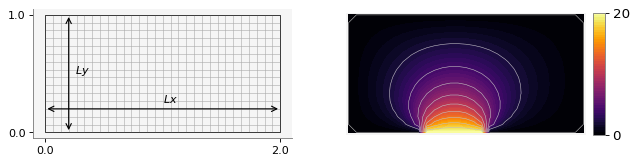
\includegraphics{08_Sol_Sis_Lin_Krylov_files/figure-pdf/cell-10-output-1.png}

Observamos un paraboloide cuyo mínimo es la solución del sistema. Esto
es más claro si graficamos los contornos de \(f(\mathbf{x})\):

\begin{Shaded}
\begin{Highlighting}[]
\NormalTok{grafica(x, y1, y2, sol, vA }\OperatorTok{=}\NormalTok{ vA, xg }\OperatorTok{=}\NormalTok{ xg, yg }\OperatorTok{=}\NormalTok{ yg, z }\OperatorTok{=}\NormalTok{ z)}
\end{Highlighting}
\end{Shaded}

\includegraphics{08_Sol_Sis_Lin_Krylov_files/figure-pdf/cell-11-output-1.png}

\section{Algoritmo de descenso por el
gradiente.}\label{algoritmo-de-descenso-por-el-gradiente.}

Este algoritmo utiliza la dirección del gradiente, en sentido negativo,
para encontrar el mínimo y la solución del sistema:

\$

\begin{array}{l}
\text{Input} : \mathbf{x}_0, tol \\
\mathbf{r}_0 = \mathbf{b}-A\mathbf{x}_0 \\
k = 0 \\
\text{WHILE}(\mathbf{r}_k > tol) \\
\qquad \mathbf{r}_k \leftarrow \mathbf{b}-A\mathbf{x}_k \\
\qquad \alpha_k \leftarrow \dfrac{\mathbf{r}_k^T\mathbf{r}_k}{\mathbf{r}_k^T A \mathbf{r}_k} \\
\qquad \mathbf{x}_{k+1} \leftarrow \mathbf{x}_k + \alpha_k \mathbf{r}_k \\
\qquad k \leftarrow k + 1 \\
\text{ENDWHILE}
\end{array}

\$

\section{Implementación.}\label{implementaciuxf3n.-3}

\begin{Shaded}
\begin{Highlighting}[]
\KeywordTok{def}\NormalTok{ steepest(A,b,xi, yi,tol,kmax):}
    \CommentTok{\# Solución inicial en forma de vector}
\NormalTok{    x }\OperatorTok{=}\NormalTok{ np.array([xi, yi]) }
    
    \CommentTok{\# Arreglos para almacenar los pasos.}
\NormalTok{    xs, ys }\OperatorTok{=}\NormalTok{ [xi], [yi]}
    
    \CommentTok{\# Solución exacta}
\NormalTok{    xe }\OperatorTok{=}\NormalTok{ np.array([}\DecValTok{2}\NormalTok{, }\OperatorTok{{-}}\DecValTok{2}\NormalTok{]) }
                  
\NormalTok{    r }\OperatorTok{=}\NormalTok{ b.T }\OperatorTok{{-}}\NormalTok{ A }\OperatorTok{@}\NormalTok{ x}
\NormalTok{    res }\OperatorTok{=}\NormalTok{ np.linalg.norm(r, }\DecValTok{2}\NormalTok{)}
\NormalTok{    res\_list }\OperatorTok{=}\NormalTok{ []}
\NormalTok{    error }\OperatorTok{=}\NormalTok{ []}
\NormalTok{    k }\OperatorTok{=} \DecValTok{0}
    \ControlFlowTok{while}\NormalTok{(res }\OperatorTok{\textgreater{}}\NormalTok{ tol }\KeywordTok{and}\NormalTok{ k }\OperatorTok{\textless{}}\NormalTok{ kmax):}
\NormalTok{        alpha }\OperatorTok{=}\NormalTok{ r.T }\OperatorTok{@}\NormalTok{ r }\OperatorTok{/}\NormalTok{ (r.T }\OperatorTok{@}\NormalTok{ A }\OperatorTok{@}\NormalTok{ r)}
\NormalTok{        x }\OperatorTok{=}\NormalTok{ x }\OperatorTok{+}\NormalTok{ r }\OperatorTok{*}\NormalTok{ alpha}
\NormalTok{        xs.append(x[}\DecValTok{0}\NormalTok{])}
\NormalTok{        ys.append(x[}\DecValTok{1}\NormalTok{])}
\NormalTok{        r }\OperatorTok{=}\NormalTok{ b.T }\OperatorTok{{-}}\NormalTok{ A }\OperatorTok{@}\NormalTok{ x}
        
        \CommentTok{\# Resido}
\NormalTok{        res }\OperatorTok{=}\NormalTok{ np.linalg.norm(r, }\DecValTok{2}\NormalTok{)}
\NormalTok{        res\_list.append(res)}
        
        \CommentTok{\# Error}
\NormalTok{        e }\OperatorTok{=}\NormalTok{ np.linalg.norm(np.array([x[}\DecValTok{0}\NormalTok{], x[}\DecValTok{1}\NormalTok{]]) }\OperatorTok{{-}}\NormalTok{ xe, }\DecValTok{2}\NormalTok{)}
\NormalTok{        error.append(e)}
        
\NormalTok{        k }\OperatorTok{+=} \DecValTok{1}
        \BuiltInTok{print}\NormalTok{(}\StringTok{\textquotesingle{}}\SpecialCharTok{\{:2d\}}\StringTok{ }\SpecialCharTok{\{:10.9f\}}\StringTok{ (}\SpecialCharTok{\{:10.9f\}}\StringTok{, }\SpecialCharTok{\{:10.9f\}}\StringTok{)\textquotesingle{}}\NormalTok{.}\BuiltInTok{format}\NormalTok{(k, e, x[}\DecValTok{0}\NormalTok{], x[}\DecValTok{1}\NormalTok{]))}
    \ControlFlowTok{return}\NormalTok{ x, np.array(xs), np.array(ys), error, res\_list, k }
\end{Highlighting}
\end{Shaded}

\section{\texorpdfstring{\textbf{Ejercicio
1.}}{Ejercicio 1.}}\label{ejercicio-1.-6}

Haciendo uso de la función \texttt{steepest()} definida en la celda
anterior, aproxima la solución del sistema de ecuaciones del Ejemplo 1.
Utiliza la solución inicial \texttt{(xi,\ yi)\ =} \((-2, 2)\), una
tolerancia \texttt{tol} = \(1 \times 10^{-5}\) y \texttt{kmax} = \(50\)
iteraciones. Utiliza las variables \texttt{solGrad}, \texttt{xs},
\texttt{ys}, \texttt{eGrad}, \texttt{rGrad} e \texttt{itGrad} para
almacenar la salida de la función \texttt{steepest()}. Posteriormente
grafica las rectas y cómo se va calculando la solución con este método.
Utiliza la función \texttt{grafica()}. Grafica también el error y el
residuo.

\begin{Shaded}
\begin{Highlighting}[]
\CommentTok{\# Solución inicial (debe darse como un arreglo tipo columna)}
\CommentTok{\# (xi, yi) = ...}

\CommentTok{\# Método Steepest descend}
\CommentTok{\# ...}

\CommentTok{\#\#\# }\RegionMarkerTok{BEGIN}\CommentTok{ SOLUTION}
\CommentTok{\# Solución inicial}
\NormalTok{(xi, yi) }\OperatorTok{=}\NormalTok{ (}\OperatorTok{{-}}\FloatTok{2.}\NormalTok{, }\FloatTok{2.}\NormalTok{)}
\NormalTok{tol }\OperatorTok{=} \FloatTok{1e{-}5}
\NormalTok{kmax }\OperatorTok{=} \DecValTok{50}

\CommentTok{\# Método Steepest descend}
\NormalTok{solGrad, xs, ys, eGrad, rGrad, itGrad  }\OperatorTok{=}\NormalTok{ steepest(A, b, xi, yi, tol, kmax)}

\CommentTok{\#file\_answer.write(\textquotesingle{}1\textquotesingle{}, solGrad, \textquotesingle{}solGrad es incorrecta: revisa la llamada y ejecución de la función steepest() así como sus parámetros de entrada.\textquotesingle{})}
\CommentTok{\#file\_answer.write(\textquotesingle{}2\textquotesingle{}, eGrad[{-}1], \textquotesingle{}eGrad[{-}1] es incorrecto: revisa la llamada y ejecución de la función steepest() así como sus parámetros de entrada.\textquotesingle{})}
\CommentTok{\#file\_answer.write(\textquotesingle{}3\textquotesingle{}, rGrad[{-}1], \textquotesingle{}rGrad[{-}1] es incorrecto: revisa la llamada y ejecución de la función steepest() así como sus parámetros de entrada.\textquotesingle{})}
\CommentTok{\#file\_answer.write(\textquotesingle{}4\textquotesingle{}, itGrad, \textquotesingle{}itGrad es incorrecto: revisa la llamada y ejecución de la función steepest() así como sus parámetros de entrada.\textquotesingle{})}

\CommentTok{\#\#\# }\RegionMarkerTok{END}\CommentTok{ SOLUTION}
\end{Highlighting}
\end{Shaded}

\begin{verbatim}
 1 3.261835423 (-1.180722892, -1.277108434)
 2 1.717502736 (0.785542169, -0.785542169)
 3 0.990340394 (1.034286544, -1.780519669)
 4 0.521458662 (1.631273044, -1.631273044)
 5 0.300681662 (1.706795433, -1.933362598)
 6 0.158322389 (1.888049165, -1.888049165)
 7 0.091291300 (1.910978854, -1.979767921)
 8 0.048068966 (1.966010108, -1.966010108)
 9 0.027717358 (1.972971893, -1.993857248)
10 0.014594433 (1.989680177, -1.989680177)
11 0.008415391 (1.991793876, -1.998134972)
12 0.004431081 (1.996866753, -1.996866753)
13 0.002555034 (1.997508502, -1.999433750)
14 0.001345340 (1.999048701, -1.999048701)
15 0.000775745 (1.999243545, -1.999828078)
16 0.000408465 (1.999711172, -1.999711172)
17 0.000235528 (1.999770329, -1.999947802)
18 0.000124016 (1.999912308, -1.999912308)
19 0.000071510 (1.999930269, -1.999984152)
20 0.000037653 (1.999973375, -1.999973375)
21 0.000021711 (1.999978829, -1.999995188)
22 0.000011432 (1.999991916, -1.999991916)
23 0.000006592 (1.999993572, -1.999998539)
24 0.000003471 (1.999997546, -1.999997546)
25 0.000002001 (1.999998048, -1.999999556)
\end{verbatim}

\begin{Shaded}
\begin{Highlighting}[]
\CommentTok{\#quizz.eval\_numeric(\textquotesingle{}1\textquotesingle{}, solGrad)}
\CommentTok{\#quizz.eval\_numeric(\textquotesingle{}2\textquotesingle{}, eGrad[{-}1])}
\CommentTok{\#quizz.eval\_numeric(\textquotesingle{}3\textquotesingle{}, rGrad[{-}1])}
\CommentTok{\#quizz.eval\_numeric(\textquotesingle{}4\textquotesingle{}, itGrad)}
\end{Highlighting}
\end{Shaded}

\textbf{Gráfica de las rectas, la solución y los pasos realizados}

\begin{Shaded}
\begin{Highlighting}[]
\NormalTok{grafica(x, y1, y2, sol, xs, ys, xg }\OperatorTok{=}\NormalTok{ xg, yg }\OperatorTok{=}\NormalTok{ yg, z }\OperatorTok{=}\NormalTok{ z)}
\end{Highlighting}
\end{Shaded}

\includegraphics{08_Sol_Sis_Lin_Krylov_files/figure-pdf/cell-15-output-1.png}

\textbf{Grafica del error y el residuo.}

\begin{Shaded}
\begin{Highlighting}[]
\CommentTok{\# Lista con el número de las iteraciones}
\NormalTok{l\_itGrad }\OperatorTok{=} \BuiltInTok{list}\NormalTok{(}\BuiltInTok{range}\NormalTok{(}\DecValTok{1}\NormalTok{,itGrad}\OperatorTok{+}\DecValTok{1}\NormalTok{)) }

\CommentTok{\# Parámetros para los ejes}
\NormalTok{a\_p }\OperatorTok{=} \BuiltInTok{dict}\NormalTok{(yscale}\OperatorTok{=}\StringTok{\textquotesingle{}log\textquotesingle{}}\NormalTok{, xlabel}\OperatorTok{=}\StringTok{\textquotesingle{}Iteraciones\textquotesingle{}}\NormalTok{, xticks }\OperatorTok{=}\NormalTok{ l\_itGrad)}

\CommentTok{\# Gráfica del error}
\NormalTok{v }\OperatorTok{=}\NormalTok{ mvis.Plotter(}\DecValTok{1}\NormalTok{,}\DecValTok{1}\NormalTok{,[a\_p]) }
\NormalTok{v.axes(}\DecValTok{1}\NormalTok{).set\_title(}\StringTok{\textquotesingle{}Error/Residuo\textquotesingle{}}\NormalTok{, loc}\OperatorTok{=}\StringTok{\textquotesingle{}left\textquotesingle{}}\NormalTok{)}
\NormalTok{v.plot(}\DecValTok{1}\NormalTok{, l\_itGrad, eGrad, marker}\OperatorTok{=}\StringTok{\textquotesingle{}.\textquotesingle{}}\NormalTok{, label}\OperatorTok{=}\StringTok{\textquotesingle{}Error\textquotesingle{}}\NormalTok{)}
\NormalTok{v.plot(}\DecValTok{1}\NormalTok{, l\_itGrad, rGrad, marker}\OperatorTok{=}\StringTok{\textquotesingle{}.\textquotesingle{}}\NormalTok{, label}\OperatorTok{=}\StringTok{\textquotesingle{}Residuo\textquotesingle{}}\NormalTok{)}
\NormalTok{v.legend()}
\NormalTok{v.grid()}
\end{Highlighting}
\end{Shaded}

\includegraphics{08_Sol_Sis_Lin_Krylov_files/figure-pdf/cell-16-output-1.png}

\section{Algoritmo de Gradiente
Conjugado}\label{algoritmo-de-gradiente-conjugado}

Este algorimo mejora al descenso del gradiente tomando direcciones
conjugadas para evitar repetir un paso en una misma dirección.

\$

\begin{array}{l}
\text{Input} : A, \mathbf{b}, \mathbf{x}_0, k_{max}, tol \\
\mathbf{d_0} = \mathbf{r}_0 = \mathbf{b} - A \mathbf{x}_0 \\ 
k = 0 \\
\text{While} (||\mathbf{r}|| > tol \quad \text{AND} \quad k < k_{max} ) \\
\qquad \alpha_k = \frac{\mathbf{r}_k^T \mathbf{r}_k}{\mathbf{d}_k^T A \mathbf{d}_k} \\
\qquad \mathbf{x}_{k+1} = \mathbf{x}_{k} + \alpha_k \mathbf{d}_{k} \\
\qquad \mathbf{r}_{k+1} = \mathbf{r}_{k} - \alpha_k A \mathbf{d}_{k} \\
\qquad \beta_{k+1} = \frac{\mathbf{r}_{k+1}^T \mathbf{r}_{k+1}}{\mathbf{r}_{k}^T \mathbf{r}_{k}}  \\
\qquad \mathbf{d}_{k+1} = \mathbf{r}_{k+1} + \beta_{k+1} \mathbf{d}_{k} \\
\qquad k = k + 1  \\
\text{End While}
\end{array}

\$

\subsection{Implementación.}\label{implementaciuxf3n.-4}

\begin{Shaded}
\begin{Highlighting}[]
\KeywordTok{def}\NormalTok{ conjugateGradient(A,b,xi, yi, tol,kmax):}
    \CommentTok{\# Solución inicial en forma de vector}
\NormalTok{    x }\OperatorTok{=}\NormalTok{ np.array([xi, yi]) }
    
    \CommentTok{\# Arreglos para almacenar los pasos.}
\NormalTok{    xs, ys }\OperatorTok{=}\NormalTok{ [xi], [yi]}
    
    \CommentTok{\# Solución exacta}
\NormalTok{    xe }\OperatorTok{=}\NormalTok{ np.array([}\DecValTok{2}\NormalTok{, }\OperatorTok{{-}}\DecValTok{2}\NormalTok{]) }

\NormalTok{    r }\OperatorTok{=}\NormalTok{ b.T }\OperatorTok{{-}}\NormalTok{ A }\OperatorTok{@}\NormalTok{ x}
\NormalTok{    d }\OperatorTok{=}\NormalTok{ r}
\NormalTok{    rk\_norm }\OperatorTok{=}\NormalTok{ r.T }\OperatorTok{@}\NormalTok{ r}
\NormalTok{    res }\OperatorTok{=}\NormalTok{ np.linalg.norm(rk\_norm)}
\NormalTok{    res\_list }\OperatorTok{=}\NormalTok{ []}
\NormalTok{    error }\OperatorTok{=}\NormalTok{ [] }

\NormalTok{    k }\OperatorTok{=} \DecValTok{0}
    \ControlFlowTok{while}\NormalTok{(res }\OperatorTok{\textgreater{}}\NormalTok{ tol }\KeywordTok{and}\NormalTok{ k }\OperatorTok{\textless{}}\NormalTok{ kmax):}
\NormalTok{        alpha }\OperatorTok{=} \BuiltInTok{float}\NormalTok{(rk\_norm) }\OperatorTok{/} \BuiltInTok{float}\NormalTok{(d.T }\OperatorTok{@}\NormalTok{ A }\OperatorTok{@}\NormalTok{ d)}
\NormalTok{        x }\OperatorTok{=}\NormalTok{ x }\OperatorTok{+}\NormalTok{ alpha }\OperatorTok{*}\NormalTok{ d}
\NormalTok{        xs.append(x[}\DecValTok{0}\NormalTok{])}
\NormalTok{        ys.append(x[}\DecValTok{1}\NormalTok{])}
\NormalTok{        r }\OperatorTok{=}\NormalTok{ r }\OperatorTok{{-}}\NormalTok{ alpha }\OperatorTok{*}\NormalTok{ A }\OperatorTok{@}\NormalTok{ d}
        
        \CommentTok{\# Residuo}
\NormalTok{        res }\OperatorTok{=}\NormalTok{ np.linalg.norm(r, }\DecValTok{2}\NormalTok{)}
\NormalTok{        res\_list.append(res)}

        \CommentTok{\# Error}
\NormalTok{        e }\OperatorTok{=}\NormalTok{ np.linalg.norm(np.array([x[}\DecValTok{0}\NormalTok{], x[}\DecValTok{1}\NormalTok{]]) }\OperatorTok{{-}}\NormalTok{ xe, }\DecValTok{2}\NormalTok{)}
\NormalTok{        error.append(e)}
        
\NormalTok{        rk\_old }\OperatorTok{=}\NormalTok{ rk\_norm}
\NormalTok{        rk\_norm }\OperatorTok{=}\NormalTok{ r.T }\OperatorTok{@}\NormalTok{ r}
\NormalTok{        beta }\OperatorTok{=} \BuiltInTok{float}\NormalTok{(rk\_norm) }\OperatorTok{/} \BuiltInTok{float}\NormalTok{(rk\_old)}
\NormalTok{        d }\OperatorTok{=}\NormalTok{ r }\OperatorTok{+}\NormalTok{ beta }\OperatorTok{*}\NormalTok{ d}
\NormalTok{        k }\OperatorTok{+=} \DecValTok{1}
        \BuiltInTok{print}\NormalTok{(}\StringTok{\textquotesingle{}}\SpecialCharTok{\{:2d\}}\StringTok{ }\SpecialCharTok{\{:10.9f\}}\StringTok{ (}\SpecialCharTok{\{:10.9f\}}\StringTok{, }\SpecialCharTok{\{:10.9f\}}\StringTok{)\textquotesingle{}}\NormalTok{.}\BuiltInTok{format}\NormalTok{(k, e, x[}\DecValTok{0}\NormalTok{], x[}\DecValTok{1}\NormalTok{]))}
    \ControlFlowTok{return}\NormalTok{ x, np.array(xs), np.array(ys), error, res\_list, k}
\end{Highlighting}
\end{Shaded}

\section{\texorpdfstring{\textbf{Ejercicio
2.}}{Ejercicio 2.}}\label{ejercicio-2.-5}

Haciendo uso de la función \texttt{conjugateGradient()} definida en la
celda anterior, aproxima la solución del sistema de ecuaciones del
Ejemplo 1. Utiliza la solución inicial \texttt{(xi,\ yi)\ =}
\((-2, 2)\), una tolerancia \texttt{tol} = \(1 \times 10^{-5}\) y
\texttt{kmax} = \(50\) iteraciones. Utiliza las variables
\texttt{solCGM}, \texttt{xs}, \texttt{ys}, \texttt{eCGM}, \texttt{rCGM}
e \texttt{itCGM} para almacenar la salida de la función
\texttt{conjugateGradient()}. Posteriormente grafica las rectas y cómo
se va calculando la solución con este método. Utiliza la función
\texttt{grafica()}. Grafica también el error y el residuo.

\begin{Shaded}
\begin{Highlighting}[]
\CommentTok{\# Solución inicial (debe darse como un arreglo tipo columna)}
\CommentTok{\# (xi, yi) = ...}

\CommentTok{\# Método CGM}
\CommentTok{\# ...}

\CommentTok{\#\#\# }\RegionMarkerTok{BEGIN}\CommentTok{ SOLUTION}
\CommentTok{\# Solución inicial}
\NormalTok{(xi, yi) }\OperatorTok{=}\NormalTok{ (}\OperatorTok{{-}}\FloatTok{2.}\NormalTok{, }\FloatTok{2.}\NormalTok{)}
\NormalTok{tol }\OperatorTok{=} \FloatTok{1e{-}5}
\NormalTok{kmax }\OperatorTok{=} \DecValTok{50}

\CommentTok{\# Método CGM}
\NormalTok{solCGM, xs, ys, eCGM, rCGM, itCGM }\OperatorTok{=}\NormalTok{ conjugateGradient(A, b, xi, yi, tol, kmax)}

\CommentTok{\#file\_answer.write(\textquotesingle{}5\textquotesingle{}, solCGM, \textquotesingle{}solCGM es incorrecta: revisa la llamada y ejecución de la función conjugateGradient() así como sus parámetros de entrada.\textquotesingle{})}
\CommentTok{\#file\_answer.write(\textquotesingle{}6\textquotesingle{}, eCGM[{-}1], \textquotesingle{}eCGM[{-}1] es incorrecto: revisa la llamada y ejecución de la función conjugateGradient() así como sus parámetros de entrada.\textquotesingle{})}
\CommentTok{\#file\_answer.write(\textquotesingle{}7\textquotesingle{}, rCGM[{-}1], \textquotesingle{}rCGM[{-}1] es incorrecto: revisa la llamada y ejecución de la función conjugateGradient() así como sus parámetros de entrada.\textquotesingle{})}
\CommentTok{\#file\_answer.write(\textquotesingle{}8\textquotesingle{}, itCGM, \textquotesingle{}itCGM es incorrecto: revisa la llamada y ejecución de la función conjugateGradient() así como sus parámetros de entrada.\textquotesingle{})}

\CommentTok{\#\#\# }\RegionMarkerTok{END}\CommentTok{ SOLUTION}
\end{Highlighting}
\end{Shaded}

\begin{verbatim}
 1 3.261835423 (-1.180722892, -1.277108434)
 2 0.000000000 (2.000000000, -2.000000000)
\end{verbatim}

\begin{Shaded}
\begin{Highlighting}[]
\CommentTok{\#quizz.eval\_numeric(\textquotesingle{}5\textquotesingle{}, solCGM)}
\CommentTok{\#quizz.eval\_numeric(\textquotesingle{}6\textquotesingle{}, eCGM[{-}1])}
\CommentTok{\#quizz.eval\_numeric(\textquotesingle{}7\textquotesingle{}, rCGM[{-}1])}
\CommentTok{\#quizz.eval\_numeric(\textquotesingle{}8\textquotesingle{}, itCGM)}
\end{Highlighting}
\end{Shaded}

\begin{Shaded}
\begin{Highlighting}[]
\NormalTok{grafica(x, y1, y2, sol, xs, ys, xg }\OperatorTok{=}\NormalTok{ xg, yg }\OperatorTok{=}\NormalTok{ yg, z }\OperatorTok{=}\NormalTok{ z)}
\end{Highlighting}
\end{Shaded}

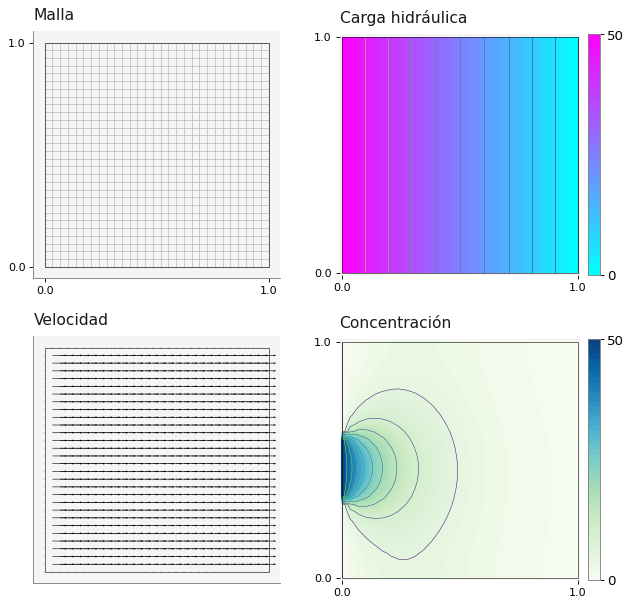
\includegraphics{08_Sol_Sis_Lin_Krylov_files/figure-pdf/cell-20-output-1.png}

\begin{Shaded}
\begin{Highlighting}[]
\CommentTok{\# Lista con el número de las iteraciones}
\NormalTok{l\_itGrad }\OperatorTok{=} \BuiltInTok{list}\NormalTok{(}\BuiltInTok{range}\NormalTok{(}\DecValTok{1}\NormalTok{,itGrad}\OperatorTok{+}\DecValTok{1}\NormalTok{)) }
\NormalTok{l\_itCGM }\OperatorTok{=} \BuiltInTok{list}\NormalTok{(}\BuiltInTok{range}\NormalTok{(}\DecValTok{1}\NormalTok{,itCGM}\OperatorTok{+}\DecValTok{1}\NormalTok{))}

\CommentTok{\# Parámetros para los ejes}
\NormalTok{a\_p }\OperatorTok{=} \BuiltInTok{dict}\NormalTok{(yscale}\OperatorTok{=}\StringTok{\textquotesingle{}log\textquotesingle{}}\NormalTok{, xlabel}\OperatorTok{=}\StringTok{\textquotesingle{}Iteraciones\textquotesingle{}}\NormalTok{, xticks }\OperatorTok{=}\NormalTok{ l\_itGrad)}

\CommentTok{\# Gráfica del error}
\NormalTok{v }\OperatorTok{=}\NormalTok{ mvis.Plotter(}\DecValTok{1}\NormalTok{,}\DecValTok{1}\NormalTok{,[a\_p]) }
\NormalTok{v.axes(}\DecValTok{1}\NormalTok{).set\_title(}\StringTok{\textquotesingle{}Error/Residuo\textquotesingle{}}\NormalTok{, loc}\OperatorTok{=}\StringTok{\textquotesingle{}left\textquotesingle{}}\NormalTok{)}

\NormalTok{v.plot(}\DecValTok{1}\NormalTok{, l\_itGrad, eGrad, marker}\OperatorTok{=}\StringTok{\textquotesingle{}.\textquotesingle{}}\NormalTok{, label}\OperatorTok{=}\StringTok{\textquotesingle{}Error Steepest\textquotesingle{}}\NormalTok{)}
\NormalTok{v.plot(}\DecValTok{1}\NormalTok{, l\_itGrad, rGrad, marker}\OperatorTok{=}\StringTok{\textquotesingle{}.\textquotesingle{}}\NormalTok{, label}\OperatorTok{=}\StringTok{\textquotesingle{}Residuo Steepest\textquotesingle{}}\NormalTok{)}
\NormalTok{v.plot(}\DecValTok{1}\NormalTok{, l\_itCGM, eCGM, marker}\OperatorTok{=}\StringTok{\textquotesingle{}.\textquotesingle{}}\NormalTok{, label}\OperatorTok{=}\StringTok{\textquotesingle{}Error CGM\textquotesingle{}}\NormalTok{)}
\NormalTok{v.plot(}\DecValTok{1}\NormalTok{, l\_itCGM, rCGM, marker}\OperatorTok{=}\StringTok{\textquotesingle{}.\textquotesingle{}}\NormalTok{, label}\OperatorTok{=}\StringTok{\textquotesingle{}Residuo CGM\textquotesingle{}}\NormalTok{)}

\NormalTok{v.legend()}
\NormalTok{v.grid()}
\end{Highlighting}
\end{Shaded}

\includegraphics{08_Sol_Sis_Lin_Krylov_files/figure-pdf/cell-21-output-1.png}

\section{\texorpdfstring{\textbf{Ejercicio
3.}}{Ejercicio 3.}}\label{ejercicio-3.-3}

Carga los archivos \texttt{errorJacobi.npy},
\texttt{errorGaussSeidel.npy} y \texttt{errorSOR.npy} en las variables
\texttt{eJ}, \texttt{eG} y \texttt{eSOR} respectivamente (utiliza la
función \texttt{np.load()}). Posteriormente grafica los errores de los 5
métodos: Jacobi, Gauss-Seidel, SOR, Steepest Descend, CGM. ¿Cuál de
todos estos métodos usarías?

\begin{Shaded}
\begin{Highlighting}[]
\NormalTok{eJ }\OperatorTok{=}\NormalTok{ np.load(}\StringTok{\textquotesingle{}errorJacobi.npy\textquotesingle{}}\NormalTok{)}
\NormalTok{eG }\OperatorTok{=}\NormalTok{ np.load(}\StringTok{\textquotesingle{}errorGaussSeidel.npy\textquotesingle{}}\NormalTok{)}
\NormalTok{eSOR }\OperatorTok{=}\NormalTok{ np.load(}\StringTok{\textquotesingle{}errorSOR.npy\textquotesingle{}}\NormalTok{)}

\CommentTok{\# Lista con el número de las iteraciones}
\NormalTok{l\_itJ }\OperatorTok{=} \BuiltInTok{list}\NormalTok{(}\BuiltInTok{range}\NormalTok{(}\DecValTok{1}\NormalTok{,}\BuiltInTok{len}\NormalTok{(eJ)}\OperatorTok{+}\DecValTok{1}\NormalTok{)) }
\NormalTok{l\_itG }\OperatorTok{=} \BuiltInTok{list}\NormalTok{(}\BuiltInTok{range}\NormalTok{(}\DecValTok{1}\NormalTok{,}\BuiltInTok{len}\NormalTok{(eG)}\OperatorTok{+}\DecValTok{1}\NormalTok{)) }
\NormalTok{l\_itSOR }\OperatorTok{=} \BuiltInTok{list}\NormalTok{(}\BuiltInTok{range}\NormalTok{(}\DecValTok{1}\NormalTok{,}\BuiltInTok{len}\NormalTok{(eSOR)}\OperatorTok{+}\DecValTok{1}\NormalTok{)) }
\NormalTok{l\_itGrad }\OperatorTok{=} \BuiltInTok{list}\NormalTok{(}\BuiltInTok{range}\NormalTok{(}\DecValTok{1}\NormalTok{,itGrad}\OperatorTok{+}\DecValTok{1}\NormalTok{)) }
\NormalTok{l\_itCGM }\OperatorTok{=} \BuiltInTok{list}\NormalTok{(}\BuiltInTok{range}\NormalTok{(}\DecValTok{1}\NormalTok{,itCGM}\OperatorTok{+}\DecValTok{1}\NormalTok{))}

\CommentTok{\# Parámetros para los ejes}
\NormalTok{a\_p }\OperatorTok{=} \BuiltInTok{dict}\NormalTok{(yscale}\OperatorTok{=}\StringTok{\textquotesingle{}log\textquotesingle{}}\NormalTok{, xlabel}\OperatorTok{=}\StringTok{\textquotesingle{}Iteraciones\textquotesingle{}}\NormalTok{, xticks }\OperatorTok{=}\NormalTok{ l\_itGrad)}

\CommentTok{\# Gráfica del error}
\NormalTok{v }\OperatorTok{=}\NormalTok{ mvis.Plotter(}\DecValTok{1}\NormalTok{,}\DecValTok{1}\NormalTok{,[a\_p]) }
\NormalTok{v.axes(}\DecValTok{1}\NormalTok{).set\_title(}\StringTok{\textquotesingle{}Error\textquotesingle{}}\NormalTok{, loc}\OperatorTok{=}\StringTok{\textquotesingle{}left\textquotesingle{}}\NormalTok{)}
\NormalTok{v.plot(}\DecValTok{1}\NormalTok{, l\_itJ, eJ, marker}\OperatorTok{=}\StringTok{\textquotesingle{}.\textquotesingle{}}\NormalTok{, label}\OperatorTok{=}\StringTok{\textquotesingle{}Jacobi\textquotesingle{}}\NormalTok{)}
\NormalTok{v.plot(}\DecValTok{1}\NormalTok{, l\_itG, eG, marker}\OperatorTok{=}\StringTok{\textquotesingle{}.\textquotesingle{}}\NormalTok{, label}\OperatorTok{=}\StringTok{\textquotesingle{}Gauss{-}Seidel\textquotesingle{}}\NormalTok{)}
\NormalTok{v.plot(}\DecValTok{1}\NormalTok{, l\_itSOR, eSOR, marker}\OperatorTok{=}\StringTok{\textquotesingle{}.\textquotesingle{}}\NormalTok{, label}\OperatorTok{=}\StringTok{\textquotesingle{}SOR\textquotesingle{}}\NormalTok{)}
\NormalTok{v.plot(}\DecValTok{1}\NormalTok{, l\_itGrad, eGrad, marker}\OperatorTok{=}\StringTok{\textquotesingle{}.\textquotesingle{}}\NormalTok{, label}\OperatorTok{=}\StringTok{\textquotesingle{}Steepest descend\textquotesingle{}}\NormalTok{)}
\NormalTok{v.plot(}\DecValTok{1}\NormalTok{, l\_itCGM, eCGM, marker}\OperatorTok{=}\StringTok{\textquotesingle{}.\textquotesingle{}}\NormalTok{, label}\OperatorTok{=}\StringTok{\textquotesingle{}Gradiente Conjugado\textquotesingle{}}\NormalTok{)}

\NormalTok{v.legend()}
\NormalTok{v.grid()}
\end{Highlighting}
\end{Shaded}

\includegraphics{08_Sol_Sis_Lin_Krylov_files/figure-pdf/cell-22-output-1.png}



\end{document}
